\documentclass{mimosis}

\usepackage{metalogo}

%%%%%%%%%%%%%%%%%%%%%%%%%%%%%%%%%%%%%%%%%%%%%%%%%%%%%%%%%%%%%%%%%%%%%%%%
% Some of my favourite personal adjustments
%%%%%%%%%%%%%%%%%%%%%%%%%%%%%%%%%%%%%%%%%%%%%%%%%%%%%%%%%%%%%%%%%%%%%%%%
%
% These are the adjustments that I consider necessary for typesetting
% a nice thesis. However, they are *not* included in the template, as
% I do not want to force you to use them.

% This ensures that I am able to typeset bold font in table while still aligning the numbers
% correctly.
\usepackage{etoolbox}

%%%%%%%%%%%%%%%%%%%%%%%%%%%%%%%%%%%%%%%%%%%%%%%%%%%%%%%%%%%%%%%%%%%%%%%%
% Hyperlinks & bookmarks
%%%%%%%%%%%%%%%%%%%%%%%%%%%%%%%%%%%%%%%%%%%%%%%%%%%%%%%%%%%%%%%%%%%%%%%%

\usepackage[%
  colorlinks = true,
  citecolor  = RedViolet,
  linkcolor  = NavyBlue,
  urlcolor   = NavyBlue,
  backref    = page
  ]{hyperref}

\renewcommand*{\backref}[1]{}
\renewcommand*{\backrefalt}[4]{%
    \ifcase #1%
          \or [cited on page~#2]%
          \else [cited on pages~#2]%
    \fi%
    }

%%%%%%%%%%%%%%%%%%%%%%%%%%%%%%%%%%%%%%%%%%%%%%%%%%%%%%%%%%%%%%%%%%%%%%%%
% Bibliography
%%%%%%%%%%%%%%%%%%%%%%%%%%%%%%%%%%%%%%%%%%%%%%%%%%%%%%%%%%%%%%%%%%%%%%%%

\usepackage[sort]{natbib}
\setcitestyle{%
    authoryear,%
    open={[},close={]},citesep={;},%
    aysep={},yysep={,},%
    notesep={, }}

% ACM bibliography style looks more professional
\bibliographystyle{ACM-Reference-Format}


%%%%%%%%%%%%%%%%%%%%%%%%%%%%%%%%%%%%%%%%%%%%%%%%%%%%%%%%%%%%%%%%%%%%%%%%
% Fonts
%%%%%%%%%%%%%%%%%%%%%%%%%%%%%%%%%%%%%%%%%%%%%%%%%%%%%%%%%%%%%%%%%%%%%%%%

\ifxetexorluatex
  \setmainfont{Minion Pro}
\else
  \usepackage[tt=false,type1=true]{libertine}
  \usepackage[varqu]{zi4}
  \usepackage[libertine]{newtxmath}
  % \usepackage[lf]{ebgaramond}
  % \usepackage[oldstyle,scale=0.7]{sourcecodepro}
  % \singlespacing
\fi

\usepackage{CJKutf8}

%%%%%%%%%%%%%%%%%%%%%%%%%%%%%%%%%%%%%%%%%%%%%%%%%%%%%%%%%%%%%%%%%%%%%%%%
% Ordinals
%%%%%%%%%%%%%%%%%%%%%%%%%%%%%%%%%%%%%%%%%%%%%%%%%%%%%%%%%%%%%%%%%%%%%%%%

\makeatletter
\@ifundefined{st}{%
  \newcommand{\st}{\textsuperscript{\textup{st}}\xspace}
}{}
\@ifundefined{rd}{%
  \newcommand{\rd}{\textsuperscript{\textup{rd}}\xspace}
}{}
\@ifundefined{nd}{%
  \newcommand{\nd}{\textsuperscript{\textup{nd}}\xspace}
}{}
\makeatother

\renewcommand{\th}{\textsuperscript{\textup{th}}\xspace}

%%%%%%%%%%%%%%%%%%%%%%%%%%%%%%%%%%%%%%%%%%%%%%%%%%%%%%%%%%%%%%%%%%%%%%%%
% Load my packages
%%%%%%%%%%%%%%%%%%%%%%%%%%%%%%%%%%%%%%%%%%%%%%%%%%%%%%%%%%%%%%%%%%%%%%%%

\usepackage{ottalt}

\renewcommand\ottaltinferrule[4]{
  \inferrule*[narrower=0.6,lab=#1,#2]
    {#3}
    {#4}
}

%%----------------------------------------------------------------------------%%


\title{Compositional Programming in Action}
\author{Yaozhu Sun}
\date{21 January 2025}


%%----------------------------------------------------------------------------%%
%%    Environment for Title Page                                              %%
%%----------------------------------------------------------------------------%%

\makeatletter
\renewcommand{\maketitle}
{%
  \begin{titlepage}
    \renewcommand{\baselinestretch}{1}
    \begin{center}
      \vspace*{\stretch{3}}
      {\huge\textsf{\textbf{\@title}}\par}
      \vspace*{1.25cm}
      {\large\textit{by}\par}
      \vspace*{1cm}
      {\Large\textbf{\@author}\par}
      {\begin{CJK}{UTF8}{mj}(孫耀珠)\end{CJK}\par}
      \vspace*{\stretch{5}}
      {{
\includegraphics[width=30mm]{figures/hku}} \par}
      {\hbox{}\par}
      \vspace*{\stretch{5}}
      {
        {\normalsize
        A thesis submitted in partial fulfillment of the requirements for \\
        the degree of Doctor of Philosophy \\
        at the University of Hong Kong \\
        \par
        }
      }
      \vspace*{\stretch{1}}
      {\large\@date\par}
      \vspace*{\stretch{1}}
    \end{center}
  \end{titlepage}
} \makeatother




%%----------------------------------------------------------------------------%%
%%    Environment for Abstract                                                %%
%%----------------------------------------------------------------------------%%

\makeatletter
\newenvironment{abstract}%
{
  \if@twocolumn
    \@restonecoltrue\onecolumn
  \else
    \@restonecolfalse\newpage
  \fi
  \pagestyle{empty}%
  \setcounter{page}\@ne
  \mbox{}
  \newpage
  \pagestyle{empty}%
  \setcounter{page}\@ne
  \cleardoublepage
  \begin{center}
  \large
  Abstract of thesis entitled            \par
  \textbf{``\@title''}                   \par
                                         \vspace*{0.2in}
  Submitted by                           \par
  \textbf{\@author}                      \par
                                         \vspace*{0.2in}
  for the degree of Doctor of Philosophy \\
  at the University of Hong Kong         \\
  on \@date
  \end{center}
  \vspace*{0.5in}
}%
{
  \if@restonecol\twocolumn \else \newpage \fi
  \if@twoside\else
  \setcounter{page}\@ne
  \fi
}
\makeatother

%%----------------------------------------------------------------------------%%
%%    Environment for Declaration                                             %%
%%----------------------------------------------------------------------------%%


\makeatletter
\newcommand{\makedeclaration}
{
\chapter*{Declaration}
\addcontentsline{toc}{chapter}{Declaration}
\noindent I declare that this thesis represents my own work, except
where due acknowledgment is made, and that it has not been
previously included in a thesis, dissertation, or report submitted
to this University or to any other institution for a degree,
diploma, or other qualifications.
\vspace*{1.5in}

\noindent%
\begin{tabular}{@{}l@{}}
\dotfill \\
\@author\hspace*{3cm}\\
\@date\\
\end{tabular}
}
\makeatother

%%----------------------------------------------------------------------------%%
%%    Environment for Acknowledgments                                         %%
%%----------------------------------------------------------------------------%%

\makeatletter
\newcommand{\makeAck}
{
\chapter*{Acknowledgments}
\addcontentsline{toc}{chapter}{Acknowledgments}
First of all, I would like to thank my PhD supervisor, Prof. Bruno C. d. S.
Oliveira, for his guidance and support throughout my studies...

I also would like to thank Prof. Jonathan Aldrich from Carnegie Mellon
University, who served as my external examiner, for his insightful comments on
my thesis...

}
\makeatother


\KOMAoptions{listof=totoc}
% \setkomafont{sectioning}{\normalfont\bfseries}

%%%%%%%%%%%%%%%%%%%%%%%%%%%%%%%%%%%%%%%%%%%%%%%%%%%%%%%%%%%%%%%%%%%%%%%%
% Incipit
%%%%%%%%%%%%%%%%%%%%%%%%%%%%%%%%%%%%%%%%%%%%%%%%%%%%%%%%%%%%%%%%%%%%%%%%

\begin{document}

\maketitle

\begin{abstract}
\noindent
Compositionality is an important principle in software engineering, meaning that
a complex system can be built by composing simpler parts. However, it is
non-trivial to achieve compositionality in practice. For example, the expression
problem poses a challenge for reconciling modularity and extensibility. CP, a
new statically typed programming language, naturally solves such challenges by
providing language-level support for compositional programming.

This thesis studies the practical aspects of CP. We first showcase why
compositional programming matters with two applications. The first one is about
embedded domain-specific languages. We show that CP enables a new embedding
technique that combines the advantages of shallow and deep embeddings and
surpasses other techniques like tagless-final embeddings by supporting modular
dependencies. The second application is about dynamic inheritance in
object-oriented programming. CP innovatively embraces a trait model with merging
and prevents implicit overloading. By comparing with type-unsafe code in
TypeScript, we show that CP supports dynamic multiple inheritance and family
polymorphism while preserving type safety.

We then present the design and implementation of the CP compiler. With novel
language features for compositionality, the efficient compilation of CP code is
non-trivial, especially when separate compilation is desired. The key idea is to
compile merges to type-indexed records, which outperforms previous work using
nested pairs. To ensure the type safety of dynamic inheritance, CP's type system
employs coercive subtyping, leading to significant slowdown in compiled code. We
mitigate the issue by several optimizations, including eliminating coercions for
equivalent types. We evaluate the impact of these optimizations using benchmarks
and show that the optimized compiler targeting JavaScript can be orders of
magnitude faster than a naive compilation scheme for merges, obtaining
performance comparable to class-based JavaScript programs.

Finally, besides ubiquitous intersection types in CP, we explore the extension
with union types, which provides a solid foundation for named and optional
arguments. Our approach avoids a critical type-safety issue in popular static
type checkers for Python and Ruby, particularly in handling first-class named
arguments in the presence of subtyping. A survey of named and optional arguments
in other languages shows that CP's design achieves a good balance of simplicity
and effectiveness.

Both the compilation scheme for CP and the encoding of named and optional
arguments are formalized in Coq and proven to be type-safe.

\vspace{1.5\baselineskip}

\noindent\makebox[\linewidth]{\rule{0.7\textwidth}{0.4pt}}

\begin{center}
\textbf{An abstract of 374 words}
\end{center}

\end{abstract}


%%---------------------%%
\frontmatter
%%---------------------%%
\makedeclaration
\makeAck
\tableofcontents
\listoffigures
\listoftables
% \listoftheorems[ignoreall, show={theorem,lemma}]

%%---------------------%%
\mainmatter
%%---------------------%%

\part{Prologue}
\chapter{Introduction} \label{ch:introduction}

This thesis focuses on the practical aspects of \emph{compositional
programming}, which is a statically typed programming paradigm that emphasizes
modularity and extensibility, proposed by Weixin Zhang, Yaozhu Sun (the author),
and Bruno C. d. S. Oliveira \citeyearpar{zhang2021compositional}. In this
chapter, we first give an overview of the motivation and contributions of this
thesis. Then, we outline the organization of this thesis.

\section{Motivation}

Modern software systems are becoming increasingly complex, with codebases
spanning millions to billions of lines of code. Such complexity escalates
development costs and maintenance efforts, making it harder to evolve software
systems. \citet{brooks1987no} claimed in his famous essay \emph{No Silver Bullet}:
\begin{quoting}
``The complexity of software is an essential property, not an accidental one.''
\end{quoting}
However, the situation is far less pessimistic nowadays. We have seen many
advances in programming languages, tools, and methodologies that help manage
complexity. Even back in 1990s, \citet{cox95no} criticized
\citeauthor{brooks1987no}'s claim and emphasized the importance of
\emph{reusable software components}. Modularity, the ability to decompose a
system into independent reusable components, is a cornerstone of managing
complexity in software engineering. Like LEGO bricks, these components are
standardized, self-contained units that snap together via precise interfaces,
requiring no modification. The principle of modularity has been widely adopted
in modern software systems. For example, the microservices
architecture~\citep{richardson2018microservices}, employed by Amazon, Netflix,
Alibaba, and many other companies, organizes a system as a collection of
fine-grained services.

The benefits of modularity are threefold. First, it reduces coupling between
components, minimizing the impact of changes in one component on others. Second,
it enhances code reuse, allowing components to be repurposed across different
projects. Third, team collaboration is facilitated by modular design, as
different team members can work on different components independently.

Modularity promises ``plug-and-play'' composition, where components can interact
with each other through well-defined interfaces. However, achieving such
compositionality in practice remains challenging. The fundamental challenges
include:

\begin{enumerate}
\item \textbf{Flexibility versus safety.} Dynamic languages like JavaScript
      allow flexible composition but lack static guarantees, while static
      languages like Java pursue type safety at the cost of flexibility.
\item \textbf{Compositional conflicts.} The composition of two components may
      lead to ambiguity, inconsistency, or unintended behavior. These conflicts
      are typically due to name clashes, interface mismatches, or semantic
      contradictions.
\item \textbf{Modular dependencies.} A component may depend on another
      component, and the dependencies between components form a complex graph,
      which may include cycles. Thus, it is challenging to manage dependencies
      modularly.
\item \textbf{Expression problem~\textnormal{\citep{wadler1998expression}}.}
      Traditional paradigms, such as object-oriented programming (OOP) and
      functional programming (FP), struggle to support two-dimensional extensibility
      -- adding new data types and new operations -- in a modular way.
\end{enumerate}
The need to address these challenges simultaneously calls for a new programming
paradigm that emphasizes compositionality. The compositional programming
paradigm and the CP language~\citep{zhang2021compositional} are an attempt to
address these challenges.

\paragraph{Type-safe dynamic inheritance.}
To better illustrate the challenges of compositionality, let us first consider
their manifestation in the realm of OOP. Modularity in OOP is often achieved via
classes, and classes can be extended or composed via inheritance. In other
words, inheritance provides a mechanism for code reuse by defining new classes
that inherit from existing ones. However, traditional inheritance mechanisms
have limitations. For example, multiple inheritance can lead to the
\emph{diamond problem}, as shown in \autoref{fig:diamond-1}, where a class
inherits from two classes that have a common ancestor. The method call
\lstinline{new D().m()} is ambiguous, as it is unclear whether it should return
\lstinline{"B"} or \lstinline{"C"}.

\begin{figure}
\begin{subfigure}{.54\textwidth}
\begin{lstlisting}[language=TypeScript]
class A { m() { return "A"; } }
class B extends A { m() { return "B"; } }
class C extends A { m() { return "C"; } }
class D extends B, C {}
new D().m() // Should it return "B" or "C"?
\end{lstlisting}
\caption{Multiple inheritance.} \label{fig:diamond-1}
\end{subfigure}
\hfill
\begin{subfigure}{.39\textwidth}
\begin{lstlisting}[language=TypeScript]
function compose(X, Y) {
  return class extends X, Y {};
}
D = compose(B, C);
new D().m()
\end{lstlisting}
\caption{Dynamic multiple inheritance.} \label{fig:diamond-2}
\end{subfigure}
\caption{The diamond problem in OOP.}
\end{figure}

Traits~\citep{ducasse2006traits} are a mechanism that addresses the diamond
problem by detecting ambiguous compositions and requiring the programmer to
resolve the conflicts explicitly. However, the detection of conflicts becomes
more challenging when dealing with dynamic inheritance, where classes (or
traits) can be composed at run time. This feature can typically be found in
languages with first-class classes~\citep{takikawa2012gradual,lee2015theory}.
\autoref{fig:diamond-2} shows an example of the diamond problem with dynamic
multiple inheritance. Since we know nothing about the classes \lstinline{X} and
\lstinline{Y} until the function \lstinline{compose} is called, it is difficult
to detect the ambiguity in advance. Similar code can cause more severe issues
that break type safety. As a result, most statically typed languages only
provide static inheritance to achieve type safety at the cost of flexibility.

The diamond problem manifests the challenges of compositionality in OOP,
especially the aforementioned 1\st (\emph{flexibility versus safety}) and 2\nd
(\emph{compositional conflicts}) points. Ideally, an OOP language should be
flexible so that highly dynamic patterns of inheritance are allowed. At the same
time, it should be type-safe and can identify conflicts statically, so that type
errors and semantic ambiguities are prevented at compile time. It is interesting
to see whether and how the CP language can address these challenges.

\paragraph{Embedded domain-specific languages.}
The difficulty of compositionality also arises in the context of domain-specific
languages (DSLs). A DSL is a programming language tailored to a specific domain,
such as database queries, web development, and document authoring. DSLs can be
external or internal~\citep{ghosh2010dsls}. External DSLs are standalone
languages with their own syntax and semantics, such as SQL, HTML, and CSS.
Internal DSLs are typically embedded in a host language, such as parser
combinators~\citep{leijen2001parsec} and fluent
interfaces~\citep{fowler2005fluent}. There are several well-known techniques to
do such embeddings, including \emph{deep} and \emph{shallow}
embeddings~\citep{boulton1992experience}.

If we take a minimal DSL with numbers and addition as an example, deep and
shallow embeddings are implemented in \autoref{fig:embeddings}. In a deep
embedding, the abstract syntax tree of the DSL is represented as a data type
(e.g. \lstinline{Exp}), and the semantics of the DSL are defined by an
interpreter (e.g. \lstinline{eval}). In a shallow embedding, there is no
explicit data type for the DSL; the DSL is defined directly in terms of its
semantics (e.g. \lstinline{lit} and \lstinline{add} for evaluation).

\begin{figure}
\hspace{.06\textwidth}
\begin{subfigure}{.41\textwidth}
\begin{lstlisting}[language=Haskell]
data Exp where
  Lit :: Int -> Exp
  Add :: Exp -> Exp -> Exp

eval :: Exp -> Int
eval (Lit n) = n
eval (Add l r) = eval l + eval r
\end{lstlisting}
\caption{Deep embedding.}
\end{subfigure}
\hspace{.06\textwidth}
\begin{subfigure}{.31\textwidth}
\begin{lstlisting}[language=Haskell]
type Exp = Int

lit :: Int -> Exp
lit n = n

add :: Exp -> Exp -> Exp
add l r = l + r
\end{lstlisting}
\caption{Shallow embedding.}
\end{subfigure}
\caption{Deep and shallow embeddings of a minimal DSL.} \label{fig:embeddings}
\end{figure}

The two approaches have different trade-offs. Deep embeddings support
definitions by pattern matching, including optimizations and transformations
over the abstract syntax, and allow for multiple interpretations. Shallow
embeddings have the ability to reuse host-language optimizations in the DSL and
easily add new DSL constructs. Owing to these trade-offs, many embedded DSLs end
up using a mix of approaches in practice, requiring a substantial amount of
code, as well as some advanced coding techniques. What is worse, if one
interpretation of the DSL depends on another, there is no easy way in existing
embedding techniques to decouple them and maintain modularity. These challenges
manifest the 3\rd (\emph{modular dependencies}) and 4\th (\emph{the expression
problem}) points mentioned earlier and motivate us to explore a new embedding
technique that not only combines the advantages of deep and shallow embeddings
but also supports modular dependencies.

\paragraph{The 5\th challenge: efficient compilation for CP.}
While previous work on compositional programming enables a solution to the four
challenges of compositionality, a critical gap remains in terms of practical
implementability -- specifically, how to achieve efficient compilation with
separate compilation. To date, the only implementation of the CP language is
based on an interpreter, which, while functional, does not provide the
performance necessary for practical applications.

It is non-trivial to compile CP efficiently and separately because CP supports
several novel features that are not present in mainstream programming languages.
As mentioned earlier, \emph{dynamic inheritance} and \emph{compositional
embeddings} are two key features of compositional programming. They already pose
significant challenges to type-safe compilation, let alone efficiency and
separate compilation. Another challenging feature is \emph{nested
composition}~\citep{bi2018essence}. This feature enables a form of family
polymorphism~\citep{ernst2001family}, providing an elegant solution to the
expression problem~\citep{ernst2004expression}, so it is crucial to modularity
and extensibility in CP. Finally, though \emph{parametric polymorphism} is a
common feature in mainstream languages, it raises additional challenges in the
context of compilation for CP. The reason why this feature is challenging is a
bit more technical: the compilation scheme for CP relies on the concrete type of
each term, while parametric polymorphism allows abstracting over types and
delays type instantiation until run time. All these features are worth further
investigation to understand how to compile CP efficiently.

Moreover, the semantics underlying compositional programming languages rely on
\emph{coercive subtyping}~\citep{luo2013coercive}, which introduces inherent
efficiency concerns, since upcasts lead to computational overhead. A naive
implementation that inserts coercions every time upcasting is needed has a
prohibitive cost, which can be \emph{orders of magnitude} slower than JavaScript
programs. Therefore, how to reduce the overhead of coercive subtyping is also an
inevitable part of the 5\th challenge.

\paragraph{Compositional programming with union types.}
The modularity and extensibility of compositional programming are supported by
intersection types from a type-theoretic perspective. It is tempting to explore
how compositional programming can be extended with union types, the dual of
intersection types. Our preliminary investigation shows that union types enable
optional arguments in CP, while named arguments are already supported by
intersection types. Named and optional arguments are prevalent features in many
existing programming
languages~\citep{garrigue2001labeled,flatt2009keyword,rytz2010named}, enhancing
code readability and flexibility. Despite widespread use, their formalization
has not been extensively studied in the literature. Especially in languages with
subtyping, such as Python and Ruby, first-class named arguments can lead to
type-safety issues. It is worthwhile to conduct a formal study of type-safe
foundations for named and optional arguments.

\section{Contributions}

\textbf{\autoref{pt:why}} mainly serves as an appetizer for the whole thesis,
presenting two applications of compositional programming that illustrate the
importance of the paradigm:
\begin{itemize}
\item \textbf{Dynamic inheritance via merging.} We identify a type-safety issue
      in TypeScript which we call the inexact superclass problem. We model
      family-polymorphic dynamic multiple inheritance as nested trait
      composition via merging in CP, which is free from the inexact superclass
      problem and semantic ambiguity by avoiding implicit overriding.
      Disjointness plays a crucial role in ensuring type safety in the presence
      of dynamic inheritance.
\item \textbf{Compositional embeddings.} Compositional programming, together
      with the CP language, enables a new form of embedding, which we call a
      compositional embedding. We reveal that compositional embeddings have most
      of the advantages of shallow and deep embeddings. We also make a detailed
      comparison between compositional embeddings and various other techniques
      used in embedded language implementations, including hybrid, polymorphic,
      and tagless-final embeddings.
\end{itemize}
The main body of this thesis significantly improves the implementation of the CP
language in several aspects:\footnote{The latest version of CP is available at
\url{https://github.com/yzyzsun/CP-next}.}
\begin{itemize}
\item \textbf{In-browser interpreter and the \ExT DSL.} We reimplement CP as an
      in-browser interpreter. On top of this, we implement a DSL for document
      authoring called \ExT as a realistic instance of compositional embeddings.
      \ExT is extremely flexible and customizable by users, with many features
      implemented in a modular way. We have built several applications with
      \ExT, three of which are discussed in more detail in this thesis. The
      largest application is Minipedia, and the other two applications
      illustrate computational graphics like fractals and a document extension
      for charts.\footnote{The online editor for \ExT and its applications are
      available at \url{https://plground.org}.}
\item \textbf{Compiler from CP to JavaScript.} We implement a compiler for CP
      that targets JavaScript, supporting modular type checking and separate
      compilation. We propose an efficient compilation scheme that translates
      merges into extensible records, where types are used as record labels to
      perform lookup on merges. In our concrete implementation, records are
      modeled as JavaScript objects, and record extension is modeled by
      JavaScript's support for object extension.
\item \textbf{Several optimizations and an empirical evaluation.} We discuss
      several optimizations that we employ in the CP compiler and conduct an
      empirical evaluation to measure their impact. Besides, we benchmark the
      JavaScript code generated by our compiler together with handwritten
      JavaScript code.\footnote{The benchmark suite is available at
      \url{https://github.com/yzyzsun/CP-next/tree/toplas}.}
\item \textbf{Extension with named and optional arguments.} We further extend CP
      with union types and add support for named and optional arguments. Named
      arguments in CP are first-class values and avoid the type-safety issue in
      Python and Ruby. We show a simple example of fractals that benefits from
      named and optional arguments.
\end{itemize}
To ensure the correctness of the CP compiler and its extension, we provide the
following formalization mechanized using the Coq proof assistant:
\begin{itemize}
\item \textbf{Type-safety proofs for the compilation scheme.} We formalize the
      compilation scheme as an elaboration from the \lambdaiplus
      calculus~\citep{bi2018essence,huang2021taming} to a calculus with
      extensible records called \lambdar and prove the type safety
      thereof.\footnote{The Coq formalization is available at
      \url{https://github.com/yzyzsun/CP-next/tree/main/theories}.}
\item \textbf{Type-safety proofs for named and optional arguments.} We formalize
      the encoding of named and optional arguments as an elaboration from a
      minimal functional language called \uaena to a core calculus with
      intersection and union types called \lambdaiu~\citep{rehman2023blend} and
      prove the type safety thereof.\footnote{The Coq formalization is available
      at \url{https://github.com/yzyzsun/lambda-iu}.}
\end{itemize}

\section{Organization}

\begin{description}
\item[\autoref{pt:prologue}] is the prologue. \autoref{ch:introduction}
      motivates this thesis and outlines its organization.
\item[\autoref{pt:background}] provides background information.
      \autoref{ch:background} introduces intersection and union types, merges,
      disjointness, and traits. \autoref{ch:cp} gives a crash course in the CP
      language, which implements the compositional programming paradigm.
\item[\autoref{pt:why}] explains why compositional programming matters. We
      illustrate the reasons with two applications of compositional programming
      in this part: \autoref{ch:inheritance} presents a type-safe approach to
      dynamic inheritance via merging in CP; \autoref{ch:embedding} proposes a
      new embedding technique for domain-specific languages.
\item[\autoref{pt:compile}] focuses on the compilation of compositional
      programming. \autoref{ch:key} describes the key ideas in our compilation
      scheme and its implementation in the CP compiler. \autoref{ch:calculi}
      formalizes a simplified version of the compilation scheme along some of
      the key ideas. \autoref{ch:compilation} explains implementation details,
      including the JavaScript code that is generated and some core
      optimizations in the CP compiler. \autoref{ch:empirical} provides an
      empirical evaluation.
\item[\autoref{pt:union}] further extends the CP language with union types.
      \autoref{ch:arguments} shows that this extension enables a type-safe
      encoding of named and optional arguments.
\item[\autoref{pt:epilogue}] is the epilogue. \autoref{ch:related} discusses
      related work, while \autoref{ch:conclusion} concludes this thesis and
      outlines future work.
\end{description}

\pagebreak

\paragraph{Prior publications.}
The main content of this thesis is based on three of my papers.
\autoref{ch:embedding} is based on a conference paper:
\begin{itemize}
\item Yaozhu Sun, Utkarsh Dhandhania, and Bruno C.~d.~S.~Oliveira. 2022.
\textbf{Compositional Embeddings of Domain-Specific Languages}. In OOPSLA
\textit{(ACM SIGPLAN International Conference on Object-Oriented Programming
Systems, Languages, and Applications)}.
\end{itemize}
\autoref{ch:arguments} is based on another conference paper:
\begin{itemize}
\item Yaozhu Sun and Bruno C.~d.~S.~Oliveira. 2025.
\textbf{Named Arguments as Intersections, Optional Arguments as Unions}.
In ESOP \textit{(European Symposium on Programming)}.
\end{itemize}
\autoref{ch:inheritance} and the whole \autoref{pt:compile} are based on an
unpublished paper:
\begin{itemize}
\item Yaozhu Sun, Xuejing Huang, and Bruno C.~d.~S.~Oliveira. 2025.
\textbf{Type-Safe Compilation of Dynamic Inheritance via Merging}.
In submission to \textit{ACM Transactions on Programming Languages and Systems}.
\end{itemize}
In addition, \autoref{ch:cp} in the background part also adapts some material
about modular dependencies from my co-authored journal paper:
\begin{itemize}
\item Weixin Zhang, Yaozhu Sun, and Bruno C.~d.~S.~Oliveira. 2021.
\textbf{Compositional Programming}. \textit{ACM Transactions on Programming
Languages and Systems}.
\end{itemize}

\chapter{Disjoint Intersection Types and Traits} \label{ch:background}

This part provides a brief introduction to the background of this thesis. We
first introduce intersection and union types, merging, disjointness, and traits
in this chapter, laying the type-theoretic foundation for the CP language. Next
in \autoref{ch:cp}, we will give a crash course in CP in a friendly manner.

\newcommand{\tand}{\,\&\,}
\newcommand{\tor}{\,|\,}
\newcommand{\sub}{\;<:\;}

\section{Intersection Types}

Generics or parametric polymorphism provides a mechanism for code reuse by
assigning infinite possibilities of types to a single definition. This kind of
polymorphism is \emph{uniform} in that all possibilities behave identically
despite different types instantiated.

In contrast, intersection types allows explicitly enumerating all possible types
that a single definition can have. In recently developed
theories~\citep{dunfield2014elaborating,castagna2023programming}, intersection
types are closely related to overloading or \emph{ad-hoc} polymorphism. For
example, the type of the addition operator \lstinline{(+)} for both integers and
floating-point numbers can be written as:
\begin{equation*}
(\mathbf{Int} \times \mathbf{Int} \to \mathbf{Int}) \quad\&\quad
(\mathbf{Double} \times \mathbf{Double} \to \mathbf{Double})
\end{equation*}
Note that the two versions of addition do not necessarily have the same
behavior. Semantic subtyping~\citep{frisch2008semantic} provides a
set-theoretic foundation for overloaded functions typed as intersections and is
employed in the Elixir type system~\citep{castagna2023design}.

However, this connection is not the original motivation for intersection types
(the connection did not even hold!) if we look back at the history from
1970s~\citep{bono2020tale}. Instead, functions with intersection types had
uniform behavior and could be regarded as a finite portion of parametrically
polymorphic functions. This notion is called \emph{coherent} overloading or
\emph{finitary} polymorphism~\citep{pierce1991programming}, which is a limited
form of ad-hoc polymorphism. Nevertheless, intersection types are useful for
some functions that cannot be typed in the simply typed $\lambda$-calculus (\`a
la Curry), such as the $\Omega$-combinator ($\lambda x.\ x\ x$). The
$\Omega$-combinator can be typed using the two elimination rules for
intersection types in \autoref{fig:typ-and} (\textsc{T-Abs} and \textsc{T-App}
are standard rules for functions and thus omitted):
\begin{mathpar}
\inferrule*[right=T-Abs]{\inferrule*[right=T-App]{\inferrule[T-AndElimL]{\dots}
                                                                        {x : (A \to B) \tand A \;\vdash\; x : A \to B} \\
                                                  \inferrule[T-AndElimR]{\dots}
                                                                        {x : (A \to B) \tand A \;\vdash\; x : A}}
                                                 {x : (A \to B) \tand A \;\vdash\; x\ x : B}}
                        {\cdot \vdash \lambda x.\ x\ x : (A \to B) \tand A \to B}
\end{mathpar}
Intersection types in this setting are typically used to characterize the
termination properties of $\lambda$-terms~\citep{dezani2005compositional}.
Because of the correspondence with termination, type inference with intersection
types is \emph{not} decidable; neither is type
inhabitation~\citep{urzyczyn1999emptiness}.

In light of the analogy with set intersection, it is tempting to add subtyping
to an intersection type system. \autoref{fig:sub-and} shows three subtyping
rules for intersection types, which are naturally induced by set inclusion.
Besides the subtyping rules, we also need to add the standard subsumption rule
to the typing rules in \autoref{fig:typ-and}:
\begin{mathpar}
\inferrule[T-Sub]{e : A \\ A <: B}
                 {e : B}
\end{mathpar}
With \textsc{T-Sub}, the previous elimination rules \textsc{T-AndElimL} and
\textsc{T-AndElimR} can now be derived from the subtyping rules \textsc{S-AndL}
and \textsc{S-AndR}.

\begin{figure}[t]
\begin{mathpar}
\inferrule[T-AndIntro]{e : A \\ e : B}
                      {e : A \tand B}

\inferrule[T-AndElimL]{e : A \tand B}
                      {e : A}

\inferrule[T-AndElimR]{e : A \tand B}
                      {e : B}
\end{mathpar}
\caption{Typing rules for intersection types.} \label{fig:typ-and}
\end{figure}

\begin{figure}[b]
\begin{mathpar}
\inferrule[S-AndL]{}{A \tand B \sub A}

\inferrule[S-AndR]{}{A \tand B \sub B}

\inferrule[S-And]{A <: B \\ A <: C}
                 {A \sub B \tand C}
\end{mathpar}
\caption{Subtyping rules for intersection types.} \label{fig:sub-and}
\end{figure}

\paragraph{Distributive subtyping.}
It is well known that $\lambda$-calculi have a close relationship with logical
systems~\citep{wadler2015propositions}: the Curry-Howard
isomorphism states that propositions are types and proofs are terms. An
interesting property in logic is that implication is left-distributive over
conjunction, as shown in the following equivalence:
\begin{equation*}
A \to B \land C \quad\Longleftrightarrow\quad (A \to B) \land (A \to C)
\end{equation*}
Since implication corresponds to function types and conjunction corresponds to
intersection types in our setting, the distributive property can be interpreted
as two subtyping rules:
\begin{align}
          A \to B \tand C \quad <:& \quad (A \to B) \tand (A \to C) \label{eq:dist-1} \\
(A \to B) \tand (A \to C) \quad <:& \quad A \to B \tand C \label{eq:dist-2}
\end{align}
\autoref{eq:dist-1} can be derived from the aforementioned subtyping rules for
intersection types:
\begin{mathpar}
\small
\inferrule*[right=S-And]
  {\inferrule*[left=S-Fun]{A <: A \\
                           \inferrule*[right=S-AndL]{ }
                                                    {B \tand C \sub B}}
                          {A \to B \tand C \sub A \to B} \\
   \inferrule*[right=S-Fun]{A <: A \\
                            \inferrule*[right=S-AndR]{ }
                                                     {B \tand C \sub C}}
                           {A \to B \tand C \sub A \to C}}
  {A \to B \tand C \sub (A \to B) \tand (A \to C)}
\end{mathpar}
However, \autoref{eq:dist-2} is not derivable so far. Instead, it is a key rule
of distributive subtyping, originating from the BCD type assignment
system~\citep{barendregt1983filter}. An interesting consequence of adding
\autoref{eq:dist-2} is that $(A \to B) \tand (C \to D)$ is a subtype of $A \tand
C \to B \tand D$. This can be derived as follows via transitivity:
\begin{mathpar}
\text{(I)}
\footnotesize
\inferrule*[right=S-And]{\inferrule*[left=S-AndL]{\inferrule*[left=S-Fun]{A \tand C <: A \\ B <: B}
                                                                         {A \to B \sub A \tand C \to B}}
                                                 {(A \to B) \tand (C \to D) <: A \tand C \to B} \\
                         \inferrule*[right=S-AndR]{\inferrule*[right=S-Fun]{A \tand C <: C \\ D <: D}
                                                                           {C \to D \sub A \tand C \to D}}
                                                  {(A \to B) \tand (C \to D) <: A \tand C \to D}}
                        {(A \to B) \tand (C \to D) \sub (A \tand C \to B) \tand (A \tand C \to D)}

\normalsize
\inferrule*[right=S-Trans]
  {\text{(I)}  \quad (A \to B) \tand (C \to D) \sub (A \tand C \to B) \tand (A \tand C \to D) \\
   \text{(II)} \quad (A \tand C \to B) \tand (A \tand C \to D) \sub A \tand C \to B \tand D}
  {(A \to B) \tand (C \to D) \sub A \tand C \to B \tand D}
\end{mathpar}
Judgment (I) is derivable as shown above, and Judgment (II) directly follows
\autoref{eq:dist-2}. In short, distributive subtyping allows using an
intersection of two function types as if it is a function type with the two
parameter types intersected and the two return types intersected. This form of
distributivity can be extended to record types and reveals the essence of nested
composition~\citep{bi2018essence}. As a result, family
polymorphism~\citep{ernst2001family} can be achieved, providing an elegant
solution to the expression
problem~\citep{wadler1998expression,ernst2004expression}. A detailed discussion
about family polymorphism in CP can be found in \autoref{sec:ep}.

\paragraph{Interaction with mutable references.}
Although distributive intersection subtyping is powerful, it poses a significant
challenge for type safety when mutable references are involved. In fact,
intersection subtyping alone without distributivity is already problematic.
\citet{davies2000intersection} illustrated the problem with the following
example, assuming that \lstinline[morekeywords=Pos]{Pos} (positive numbers) is a
subtype of \lstinline[morekeywords=Nat]{Nat} (natural numbers):
\begin{lstlisting}[morekeywords={Nat,Pos}]
let x = ref 48 : Ref Nat & Ref Pos in
let y = (x := 0) in    -- x is used as Ref Nat
let z = !x in z : Pos  -- x is used as Ref Pos
\end{lstlisting}
The code is well-typed but could cause a runtime error, because \lstinline{z} is
expected to be positive while it is actually a non-positive natural number
\lstinline{0}. The solution proposed by \citeauthor{davies2000intersection} is a
variant of \emph{value restriction}~\citep{wright1995simple}, which requires
that the introduction rule of intersection types (i.e. \textsc{T-AndIntro} in
\autoref{fig:typ-and}) only applies to values. By this means, \lstinline{ref 1}
cannot be typed as \lstinline[morekeywords={Nat,Pos}]{Ref Nat & Ref Pos} since
it is not a value. However, this solution does not work well with distributive
subtyping. \citeauthor{davies2000intersection} showed a similar example to the
previous one:
\begin{lstlisting}[morekeywords={Nat,Pos}]
let x = (\() -> ref 48) () : Ref Nat & Ref Pos in
let y = (x := 0) in    -- x is used as Ref Nat
let z = !x in z : Pos  -- x is used as Ref Pos
\end{lstlisting}
Since the anonymous function \lstinline{(\() -> ref 48)} is a value,
it can be typed as an intersection type
\lstinline[morekeywords={Nat,Pos}]{(() -> Ref Nat) & (() -> Ref Pos)}.
Besides, this function can be used as
\lstinline[morekeywords={Nat,Pos}]{() -> Ref Nat & Ref Pos}
via distributive subtyping. Applying it to \lstinline{()} yields almost the same
code as the previous example. To address this type-safety issue,
\citeauthor{davies2000intersection} have to drop the distributivity rule.

Recently, \citet{ye2024imperative} proposed a simpler solution to this problem
based on \emph{bidirectional typing}~\citep{dunfield2021bidirectional}.
Bidirectional type system divides traditional type assignment ($e : A$) into two
modes: type checking ($e \Leftarrow A$) and type inference ($e \Rightarrow a$).
The key idea of \citeauthor{ye2024imperative}'s solution is that the type of the
value stored in a reference can only be inferred but not checked:
\begin{mathpar}
\inferrule[T-Ref-Before]{e : A}
                 {\mathbf{ref}\ e : \mathbf{Ref}\ A}

\inferrule[T-Ref-After]{e \Rightarrow A}
                 {\mathbf{ref}\ e \Rightarrow \mathbf{Ref}\ A}
\end{mathpar}
With the rule \textsc{T-Ref-After}, \lstinline{ref 48} can only have type
\lstinline[morekeywords=Pos]{Ref Pos} because \lstinline{48} is inferred to have
type \lstinline[morekeywords=Pos]{Pos}. Morever, \lstinline{ref 48} cannot be
checked against \lstinline[morekeywords=Nat]{Ref Nat} since reference types are
invariant. As a result, the previous two examples cannot type-check in this
bidirectional type system. A final note is that, to have a reference of type
\lstinline[morekeywords=Nat]{Ref Nat} with the initial value \lstinline{48},
one can write \lstinline[morekeywords=Nat]{ref (48 : Nat)} instead.

\section{Merging and Disjointness}

In last section, we have mentioned that intersection types correspond to logical
conjunction when introducing distributive subtyping. However, this
correspondence does not apply to the original intersection type systems,
including the BCD system~\citep{barendregt1983filter}. \citet{hindley1983coppo}
gave a counterexample showing that some uninhabited intersection types are
provable in most logics. The root cause is that the introduction rule
(\textsc{T-AndIntro} in \autoref{fig:typ-and}) requires the two premises to have
the same term $e$, which is not the case in logical conjunction.
\citet{dunfield2014elaborating} proposed to add a merge construct ($e_1 \bbcomma
e_2$), where the comma\footnote{We use a single comma in this thesis instead of
double commas used by \citet{dunfield2014elaborating}. Although it is styled as
$\bbcomma$ in formulas, it is written as a plain comma \lstinline{,} in CP
code.} $(\bbcomma)$ is called the merge operator, to close the gap between
intersection types and logical conjunction. Two typing rules (\textsc{T-MergeL}
and \textsc{T-MergeR}) are added by \citeauthor{dunfield2014elaborating}, and
together with \textsc{T-AndIntro}, we can show that $e_1 \bbcomma e_2$ has type
$A \tand B$ if $e_1$ has type $A$ and $e_2$ has type $B$:
\begin{mathpar}
\inferrule*[lab=T-MergeL]{e_1 : A}
                         {e_1 \bbcomma e_2 : A}

\inferrule*[lab=T-MergeR]{e_2 : B}
                         {e_1 \bbcomma e_2 : B}

\inferrule*[right=T-AndIntro]{\inferrule*[left=T-MergL]{e_1 : A}
                                                       {e_1 \bbcomma e_2 : A} \\
                              \inferrule*[right=T-MergL]{e_2 : B}
                                                        {e_1 \bbcomma e_2 : B}}
                             {e_1 \bbcomma e_2 : A \tand B}
\end{mathpar}
The merge operator can be traced back to Forsythe, a ALGOL-like language
designed by \citet{reynolds1997design}. Merging in Forsythe is biased to avoid
semantic ambiguity. For example, if $f$ is a function, $e \bbcomma f$ will
override all function components in $e$. Consequently, merging in Forsythe
cannot be used to encode function overloading, though intersections of function
types are supported and a limited form of \emph{coherent} overloading can be
achieved. A significant outcome of merging is the ability to encode multi-field
records, where width and permutation subtyping are naturally supported via
intersection subtyping.

Contrary to Forsythe, merging in \citeauthor{dunfield2014elaborating}'s system
has the nice property of \emph{commutativity}: the order of merging does not
matter. Since there is no bias in favor of either side, semantic ambiguity
becomes an important problem. For example, applying
$(\lambda x.\ x + 1)\bbcomma(\lambda x.\ x + 2)$ to $0$ can yield either $1$ or
$2$. To address this issue, \citet{oliveira2016disjoint} require that the two
terms to be merged must have \emph{disjoint} types. A typical typing rule for
disjoint merges is as follows:
\begin{mathpar}
\inferrule[T-Merge-Disjoint]{e_1 \Rightarrow A \\ e_2 \Rightarrow B \\ A * B}
                            {e_1 \bbcomma e_2 \Rightarrow A \tand B}
\end{mathpar}
The premise $A * B$ denotes that $A$ and $B$ are disjoint. The aforementioned
example is now \emph{not} well-typed because $\mathbf{Int} \to \mathbf{Int}$ is
\emph{not} disjoint with $\mathbf{Int} \to \mathbf{Int}$ itself. More generally,
$A \to \mathbf{Int}$ is not disjoint with $B \to \mathbf{Int}$ no matter what
$A$ and $B$ are, because they have an overlapping part $A \tand B \to
\mathbf{Int}$ (or technically speaking, a common subtype). For example, consider
this overloaded function:
\begin{equation*}
(\lambda x.\ x + 1)\bbcomma(\lambda x.\ \mathbf{if}\ x\ \mathbf{then}\ 1\ \mathbf{else}\ 0)
: (\mathbf{Int} \to \mathbf{Int}) \tand (\mathbf{Bool} \to \mathbf{Int})
\end{equation*}
Applying it to $1 \bbcomma \mathbf{false}$ can yield $2$ if we choose the
left-hand side or $0$ if we choose the right-hand side. In contrast,
\emph{overloading by return type} is allowed in
\citeauthor{oliveira2016disjoint}'s system with disjoint intersection types.
For example, consider this exotically overloaded function:
\begin{equation*}
(\lambda x.\ x + 1)\bbcomma(\lambda x.\ x > 0)
: (\mathbf{Int} \to \mathbf{Int}) \tand (\mathbf{Int} \to \mathbf{Bool})
\end{equation*}
Applying it to an integer never causes ambiguity.

A more exciting application of disjoint merges is to model record concatenation.
The merge $r_1 \bbcomma r_2$ is concatenating two records if $r_1$ and $r_2$ are
non-overlapping records. The inherent difficulty of unambiguous record
concatenation with subtyping has been mentioned by
\citet{cardelli1991operations}. \citet{alpuim2017disjoint} further provide a
type-sound and coherent foundation for polymorphic record concatenation. With
parametric polymorphism, disjointness can also be used as a constraint on
quantified types, exhibiting similar expressiveness to bounded
polymorphism~\citep{xie2020row}. A detailed discussion about the interaction
among record concatenation, subtyping, and polymorphism can be found in
\autoref{sec:merge}.

\section{Union Types}

Union types are the dual concept of intersection types...

\section{Traits and Other Units of Code Reuse}

Similar to intersection types, traits are an overloaded concept in the
literature. In the CP language, we use the term \emph{trait} to refer to a
mechanism for code reuse described by \citet{ducasse2006traits}...


\part{Why Compositional Programming Matters}
\chapter{Compositional Embeddings of Domain-Specific Languages} \label{ch:embedding}

This chapter presents the second case study: compositional embeddings of
domain-specific languages (DSLs). We concentrate on how to embed DSLs in a
modular way and compose them to build larger DSLs. We first introduce existing
embedding techniques and their limitations in \autoref{sec:embed}. Then we show
in \autoref{sec:lang} that \emph{compositional embeddings} leverage the
strengths of both shallow and deep embeddings and essentially solves the
\emph{expression problem} for embedded DSLs. We validate our approach by
showcasing a compositionally embedded DSL for document authoring called \ExT in
\autoref{sec:dsl} and further evaluating it in \autoref{sec:evaluation}.

\section{Embeddings of DSLs} \label{sec:embed}

In this section, we give some background on existing approaches to embedded DSLs
and evaluate their strengths and drawbacks. We focus on \emph{shallow} and \emph{deep}
embeddings~\citep{boulton1992experience}, which are the two main alternative
forms of embeddings. We also discuss some other forms of embeddings near the end
of this section. To illustrate all these embeddings, we present programs in
Haskell, which is well known for its good support for embedded DSLs and has a
syntax close to the CP language.

\subsection{A Simple Region DSL}

Inspired by \citet{hudak1998modular} and \citet{hofer2008polymorphic}, we
consider a simple region DSL for plane geometry. To illustrate the challenges in
developing such a DSL, we consider five separate steps in the development, which
illustrate various desired features, such as linguistic reuse and the ease of
adding features for software evolution.

\begin{enumerate}
\item \textbf{Initial system.}
      We start with a small region language with five constructs:
      \lstinline{circle} for creating a circular region with a given radius,
      \lstinline{outside} for a complement to a certain region,
      two set operators \lstinline{union} and \lstinline{intersect}, and finally
      \lstinline{translate} for moving a region by a given vector.
      The initial interpretation is to simply calculate the syntactic size of a region.
\item \textbf{Linguistic reuse.}
      We create a region with structure sharing to assess the difficulty of
      reusing host-language optimizations.
\item \textbf{Extensibility with new constructs.}
      We extend the region language with three more constructs:
      \lstinline{univ} for the universal region that contains all points,
      \lstinline{empty} for the empty region that contains no points, and
      \lstinline{scale} for resizing a region by two scale factors in a vector.
\item \textbf{Extensibility with new operations.}
      We add a new interpretation that checks whether a given point resides in a region.
\item \textbf{Complex interpretations, transformations, and optimizations.}
      Last but not least, we discuss three kinds of more complex interpretations
      that illustrate dependent interpretations (i.e.~interpretations that need
      to call other interpretations in their implementations) and
      transformations over the AST of the region language. 
\end{enumerate}

\subsection{Initial System}

\begin{figure}
\begin{lstlisting}[language=Haskell,basicstyle=\ttfamily\footnotesize]
data Vector = Vector { x :: Double, y :: Double } deriving Show
\end{lstlisting}
\begin{subfigure}[b]{.5\textwidth}
\begin{lstlisting}[language=Haskell,deletekeywords={union,intersect},basicstyle=\ttfamily\footnotesize]
type Region = Int

circle :: Double -> Region
circle _  =  1

outside :: Region -> Region
outside a  =  a + 1

union :: Region -> Region -> Region
union a b  =  a + b + 1

intersect :: Region -> Region -> Region
intersect a b  =  a + b + 1

translate :: Vector -> Region -> Region
translate _ a  =  a + 1
\end{lstlisting}
\caption{A shallow embedding.}
\end{subfigure}%
\begin{subfigure}[b]{.5\textwidth}
\begin{lstlisting}[language=Haskell,basicstyle=\ttfamily\footnotesize]
data Region where
  Circle    :: Double -> Region
  Outside   :: Region -> Region
  Union     :: Region -> Region -> Region
  Intersect :: Region -> Region -> Region
  Translate :: Vector -> Region -> Region


size :: Region -> Int
size (Circle      _) = 1
size (Outside     a) = size a + 1
size (Union     a b) = size a + size b + 1
size (Intersect a b) = size a + size b + 1
size (Translate _ a) = size a + 1
\end{lstlisting}
\caption{A deep embedding.} \label{fig:pattern}
\end{subfigure}
\caption{The initial system for the region DSL.} \label{fig:initial}
\end{figure}

\noindent
\autoref{fig:initial} shows the definitions of the initial DSL, including the
language interface and a simple interpretation for shallow and deep embeddings.

\paragraph{Language interfaces.}
In the shallow embedding, \lstinline{Region} denotes the semantic domain. All
the five language constructs are implemented as functions (called denotation
functions), which implement the respective semantics of the language constructs.
Thus, the language interface is essentially the signature of the denotation
functions and is entangled with the definition of a particular semantic domain.
In the deep embedding, \lstinline{Region} is defined as an algebraic data
type.\footnote{We use the notation of \emph{generalized} algebraic data types to
make type annotations clear.} Algebraic data types only capture the abstract
syntax, thus enabling the language interface to be separated from any concrete
semantics.

\paragraph{Semantic interpretations.}
There can be many semantic interpretations, which associate language constructs
with their meanings. The initial semantics that we choose here is an abstract
interpretation, which calculates the syntactic size of a region (i.e.~the number
of AST nodes). We opt to have an interpretation that is slightly artificial, but
simple, so that we can focus on the key aspects of compositional embeddings. In
the shallow embedding, the semantics is defined together with the language
interface since we must specify some concrete type (\lstinline{Int} in this
case) for \lstinline{Region}. In contrast, to create a new semantic
interpretation in the deep embedding, we define a function \lstinline{size}
using pattern matching over the \lstinline{Region} data type. 

We can see that the two embeddings work quite differently: the shallow embedding
encodes semantics in region constructors, and the interpretation function from
\lstinline{Region} to \lstinline{Int} is merely the identity function; the deep
embedding does nothing concerning constructors but hands over the work to the
interpretation function \lstinline{size}.

\subsection{Linguistic Reuse and Meta-Language Optimizations} \label{sec:meta}

An important concern for embedded DSLs is \emph{linguistic
reuse}~\citep{krishnamurthi2001linguistic}. One of the key selling points of
embedded DSLs is that they can reuse much of the infrastructure of the host
language and inherit various optimizations that are available in the host
language. However, there are important differences between shallow and deep
embeddings with respect to linguistic reuse. As widely observed in previous
work~\citep{rompf2012scala,jovanovic2014yinyang,svenningsson2015combining},
shallow embeddings make linguistic reuse easier. To illustrate this, we can
create a region that contains a series of repeated subregions with horizontally
aligned circles:

\begin{lstlisting}[language=Haskell,deletekeywords={union,intersect}]
circles = go 20 (2 ** 18)
  where go :: Int -> Double -> Region
        go 0 offset = circle 1
        go n offset = let shared = go (n - 1) (offset / 2)
                      in union (translate Vector { x = -offset, y = 0 } shared)
                               (translate Vector { x =  offset, y = 0 } shared)
\end{lstlisting}

\noindent
The region \lstinline{circles} is defined via an auxiliary recursive function
\lstinline{go}. In the shallow embedding, \lstinline{shared} is of type
\lstinline{Int}, and using \lstinline{shared} twice in the \lstinline{let}-body
will avoid interpreting the region twice. The code above also works for the deep
embedding, assuming some smart constructors such as \lstinline{circle = Circle}.
However, in the deep embedding, \lstinline{shared} is an AST of type
\lstinline{Region}. In this case, the AST will be duplicated in the
\lstinline{let}-body, and later when we interpret the region, we need to
traverse the same AST twice, duplicating the size calculation. Since
\lstinline{go} is recursive, it will lead to a lot of sharing for the shallow
approach and a lot of repetition for the deep approach. As a result, the
evaluation of \lstinline{circles} is instantaneous in the shallow approach,
whereas in the deep approach, it basically does not terminate in a reasonable
amount of time. In short, in shallow embeddings, we are able to preserve sharing
by naturally exploiting the sharing optimizations present in the host language,
but sharing is lost in deep embeddings.

We should remark that this particular issue regarding sharing (which is just an
instance of linguistic reuse) is well
known~\citep{gill2009type,kiselyov2011implementing,oliveira2013abstract}. There
have been several proposed techniques that enable preserving sharing in deeply
embedded DSLs. However, all those techniques add extra complexity to the DSL
encoding, and they may even make the DSL harder to use. This is in contrast to
the shallow approach, where no extra work is required by the programmer and
host-language features are naturally reused.

\subsection{Adding More Language Constructs}

As part of evolving the DSL with additional features, we may decide to add more
constructs for regions. To evaluate how easy it is to add more language constructs,
we add three more
language constructs for the universal or empty region as well as a scaling
operator. Shallow embeddings make such extensions very easy. We only need
to add three new denotation functions:

\noindent
\begin{minipage}{0.25\textwidth}
\begin{lstlisting}[language=Haskell]
univ :: Region
univ = 1
\end{lstlisting}
\end{minipage}%
\begin{minipage}{0.25\textwidth}
\begin{lstlisting}[language=Haskell]
empty :: Region
empty = 1
\end{lstlisting}
\end{minipage}%
\begin{minipage}{0.5\textwidth}
\begin{lstlisting}[language=Haskell]
scale :: Vector -> Region -> Region
scale _ a  =  a + 1
\end{lstlisting}
\end{minipage}

\noindent
Notwithstanding the modular extension in shallow embeddings, it is awkward to
add language constructs in deep embeddings. We have to modify the algebraic data
type \lstinline{Region} and all related interpretation functions to add new
cases. This is not modular because we must change the existing code. Even if we
have access to previous definitions, it is inevitable to recompile all the code
that depends on \lstinline{Region}.

In essence, once we start adding new features, we are quickly faced with an
instance of the \emph{expression problem}~\citep{wadler1998expression}. Shallow
embeddings make adding constructs easy, whereas adding new constructs in deep
embeddings is more difficult and non-modular. As we shall see next, when adding
new semantic interpretations, we have a dual problem.

\subsection{Adding a New Interpretation} \label{sec:contains}

The syntactic size is too abstract to describe a region, so let us add a new
interpretation that checks whether a region contains a given point. For example,
a circular region of radius $r$ contains $(x,y)$ if and only if $x^2 + y^2 \le
r^2$. Although adding constructs is awkward in deep embeddings, adding a new
interpretation function is trivial:

\begin{lstlisting}[language=Haskell]
contains :: Region -> Vector -> Bool
Circle      r `contains` p  =  p.x ** 2 + p.y ** 2 <= r ** 2
Outside     a `contains` p  =  not (a `contains` p)
Union     a b `contains` p  =  a `contains` p || b `contains` p
Intersect a b `contains` p  =  a `contains` p && b `contains` p
Translate Vector {..} a `contains` p  =
                      a `contains` Vector { x = p.x - x, y = p.y - y }
\end{lstlisting}

\noindent
The code is mostly straightforward.\footnote{Two GHC language extensions are
required here: \emph{OverloadedRecordDot} and \emph{RecordWildCards}.} The only
minor remark is that we use a record wildcard (\lstinline|Vector {..}|) in the
case of \lstinline{Translate} to bring record fields (\lstinline{x} and
\lstinline{y}) into scope.

However, there is no easy modular way to support multiple interpretations in
shallow embeddings. We need to completely change the definition of
\lstinline{Region} and remap all the language constructs to a new semantic
domain. The issue of semantic extension in shallow embeddings is dual to that of
language extension in deep embeddings. To address the tension between the two
dimensions, some alternative embeddings are proposed, such as tagless-final
embeddings~\citep{carette2009finally,kiselyov2010typed} and polymorphic
embeddings~\citep{hofer2008polymorphic}, though they still have some significant
drawbacks, which will be revealed shortly.

\subsection{Dependencies, Transformations, and Complex Interpretations} \label{sec:transform}

One area where deeply embedded DSLs shine is in enabling more complex kinds of
interpretations. These interpretations may, for example, enable transformations
or rewritings on the AST, which are helpful for writing domain-specific
optimizations, among other things. For writing such complex forms of
interpretations, we often require multiple \emph{dependent} functions defined by
pattern matching, and sometimes we may even need nested pattern matching. Such
interpretations are very challenging for shallow DSLs and are often the reason
why DSL writers prefer deep embeddings.

\paragraph{Dependent interpretations.}
Let us start with a dependent interpretation that shows a text representation of
a region using a deep embedding:

\begin{lstlisting}[language=Haskell]
text :: Region -> String
text   (Circle      r)  =  "circular region of radius " ++ show r
text   (Outside     a)  =  "outside a region of size " ++ show (size a)
text s@(Union     _ _)  =
    "union of two regions of size " ++ show (size s) ++ " in total"
text s@(Intersect _ _)  =
    "intersection of two regions of size " ++ show (size s) ++ " in total"
text s@(Translate _ _)  =  "translated region of size " ++ show (size s)
\end{lstlisting}

\noindent
Note that the definition of \lstinline{text} \emph{depends} on the previously
defined \lstinline{size} function. Such a definition is challenging in shallow
embeddings. A workaround sometimes used in shallow embeddings is to use tuples
to define multiple interpretations simultaneously. For example, we can define
\lstinline{size} and \lstinline{text} together as:

\begin{lstlisting}[language=Haskell,deletekeywords={union,intersect}]
type Region = (Int, String) -- (size, text)
circle      r  =  (1, "circular region of radius " ++ show r)
outside     a  =  (fst a + 1, "outside a region of size " ++ show (fst a))
union     a b  =
    (size, "union of two regions of size " ++ show size ++ " in total")
  where size = fst a + fst b + 1
intersect a b  =
    (size, "intersection of two regions of size " ++ show size ++ " in total")
  where size = fst a + fst b + 1
translate _ a  =  (size, "translated region of size " ++ show size)
  where size = fst a + 1
\end{lstlisting}

\paragraph{Mutually dependent interpretations.} \label{sec:mutual}
A similar but more interesting example is two interpretations for checking
universality and emptiness:

\begin{lstlisting}[language=Haskell]
isUniv :: Region -> Bool
isUniv            Univ  =  True
isUniv (Outside     a)  =  isEmpty a
isUniv (Union     a b)  =  isUniv a || isUniv b
isUniv (Intersect a b)  =  isUniv a && isUniv b
isUniv (Translate _ a)  =  isUniv a
isUniv (Scale     _ a)  =  isUniv a
isUniv               _  =  False

isEmpty :: Region -> Bool
isEmpty           Empty  =  True
isEmpty (Outside     a)  =  isUniv a
isEmpty (Union     a b)  =  isEmpty a && isEmpty b
isEmpty (Intersect a b)  =  isEmpty a || isEmpty b
isEmpty (Translate _ a)  =  isEmpty a
isEmpty (Scale     _ a)  =  isEmpty a
isEmpty               _  =  False
\end{lstlisting}

\noindent
Unlike in the previous example, where only \lstinline{text} depends on
\lstinline{size}, the two definitions are \emph{mutually recursive}, depending
on each other. If we want to rewrite them using shallow embeddings, they also
have to be encoded as a pair to call each other via
\lstinline[language=Haskell]{fst} and \lstinline[language=Haskell]{snd}:

\begin{lstlisting}[language=Haskell,deletekeywords={union,intersect}]
type Region = (Bool, Bool) -- (isUniv, isEmpty)

univ           =  (True,           False)
empty          =  (False,          True)
circle      _  =  (False,          False)
outside     a  =  (snd a,          fst a)
union     a b  =  (fst a || fst b, snd a && snd b)
intersect a b  =  (fst a && fst b, snd a || snd b)
translate _ a  =  (fst a,          snd a)
scale     _ a  =  (fst a,          snd a)
\end{lstlisting}

\noindent 
Generally speaking, using tuples to deal with dependencies is non-modular and
awkward to use in that interpretations become tightly coupled. Adding more
interpretations with dependencies, for example, would require a complete rewrite
of the code: dependent interpretations have to be defined together with the
interpretations that they depend on. More advanced encodings, such as
tagless-final embeddings~\citep{kiselyov2010typed} or polymorphic
embeddings~\citep{hofer2008polymorphic}, provide ways to modularize
\emph{independent} interpretations into reusable units, but they cannot scale
well to \emph{dependent} interpretations and often have to resort to similar
techniques using tuples like the code above. In \autoref{sec:tagless}, we encode
the two examples above in tagless-final embeddings and illustrate that they
suffer from the same problems as shallow embeddings with respect to
dependencies, both mutual and non-mutual.

\paragraph{Nested pattern matching.} \label{sec:nested}
Another strength of deep embeddings is their ability to perform nested pattern
matching, which is rather useful to inspect smaller constructs. Here we take
an optimization that eliminates double negation for example. Nested pattern
matching is used to check if an \lstinline{Outside} is directly wrapped around
an outer \lstinline{Outside}. If so, both of them are eliminated; otherwise,
\lstinline{eliminate} is recursively called with inner constructs:

\begin{lstlisting}[language=Haskell]
eliminate :: Region -> Region
eliminate (Outside (Outside a))  =  eliminate a
eliminate (Outside           a)  =  Outside (eliminate a)
eliminate (Union           a b)  =  Union (eliminate a) (eliminate b)
eliminate (Intersect       a b)  =  Intersect (eliminate a) (eliminate b)
eliminate (Translate       v a)  =  Translate v (eliminate a)
eliminate (Scale           v a)  =  Scale v (eliminate a)
eliminate                     a  =  a
\end{lstlisting}

\noindent
The common use of nested pattern matching poses a second challenge to
domain-specific optimizations. \citet{kiselyov2010typed} discusses the
``\emph{seemingly impossible pattern-matching}'' problem with nested patterns,
which appear not directly encodable in tagless-final embeddings. Instead, he
proposes that such algorithms can often be implemented in a tagless-final
interpreter as context-dependent interpretations by essentially changing the
algorithm. An extra parameter is added so the semantic type looks like
\lstinline{Ctx -> repr}. However, in the general case, it is not obvious how to
convert an algorithm with nested pattern matching into one based on contexts. 

\section{Compositional Embeddings} \label{sec:lang}

After looking back at the existing embedding techniques, this section shows that
Compositional Programming enables a new form of DSL embedding called a
\emph{compositional embedding}. Compositional Programming is a statically typed
modular programming paradigm implemented by the CP language. For the details of
the semantics of CP, we refer the reader to work by
\citet{zhang2021compositional}. We have reimplemented CP as an in-browser
interpreter, which can be directly run on a serverless web page. There are some
small syntactic differences between our implementation and the original work,
which we point out when necessary. Additionally, our implementation uses the
call-by-need evaluation strategy, which optimizes the original call-by-name one.

Here, we only introduce the necessary language features of CP to illustrate
compositional embeddings. With compositional embeddings, we can get many of the
benefits of both shallow and deep embeddings without most of the drawbacks. We
revisit the challenges illustrated in \autoref{sec:embed} using our approach in
this section. A detailed comparison between compositional embeddings and various
existing forms of embeddings, including shallow, deep, hybrid, and polymorphic
embeddings, is presented at the end of this section.

\subsection{Initial System, Revisited: Compositional Interfaces and Traits}

As before, we start with an initial language interface inspired by
\citet{hudak1998modular} and an abstract interpretation that calculates the
syntactic size of a region:

\begin{lstlisting}
type Vector = { x: Double; y: Double };

type HudakSig<Region> = {
  Circle:    Double -> Region;
  Outside:   Region -> Region;
  Union:     Region -> Region -> Region;
  Intersect: Region -> Region -> Region;
  Translate: Vector -> Region -> Region;
};

type Size = { size: Int };
sz = trait implements HudakSig<Size> => {
  (Circle      _).size = 1;
  (Outside     a).size = a.size + 1;
  (Union     a b).size = a.size + b.size + 1;
  (Intersect a b).size = a.size + b.size + 1;
  (Translate _ a).size = a.size + 1;
};
\end{lstlisting}

\noindent
Since CP is also statically typed, a \emph{compositional interface}
(\lstinline{HudakSig}) serves as the specification of the DSL syntax, playing a
similar role to algebraic data types in the deep embedding. The type parameter
\lstinline{Region} is called the \emph{sort} of the interface
\lstinline{HudakSig}. Sorts can be instantiated with different concrete types
that represent different semantic domains. Every constructor, which is
capitalized, must return a sort. Compositional interfaces are implemented by
\emph{traits}~\citep{ducasse2006traits,bi2018typed}, which serve as the unit of
code reuse in CP. Traits play a similar role to classes in traditional
object-oriented languages and are used to provide implementations for
interpretations of the region DSL. To implement the abstract interpretation of
the DSL, we first define the semantic domain type \lstinline{Size}. Then we
define a trait that implements \lstinline{HudakSig<Size>}. In the body of the
trait, we use \emph{method patterns}, such as \lstinline{(Circle _).size = 1},
to define the implementation. The method patterns used in the trait body allow
us to define interpretations that look very much like the corresponding
definition of \lstinline{size} by pattern matching in Haskell in
\autoref{fig:pattern}.

\subsection{Linguistic Reuse and Meta-Language Optimizations} \label{sec:sharing}

The example of horizontally aligned circles in \autoref{sec:meta} can be
translated to CP as:

\begin{lstlisting}
sharing Region = trait [self: HudakSig<Region>] => {
  circles = letrec go (n: Int) (offset: Double): Region =
              if n == 0 then Circle 1.0
              else let shared = go (n-1) (offset/2.0)
                   in Union (Translate { x = -offset; y = 0.0 } shared)
                            (Translate { x =  offset; y = 0.0 } shared)
            in go 20 (pow 2.0 18);
};
\end{lstlisting}

\noindent
Since the region DSL can have multiple interpretations, \lstinline{circles}
should be oblivious of any concrete interpretation but only refer to the
language interface. To achieve this, we use \emph{self-type annotations}. The
trait \lstinline{sharing} is parametrized by a type parameter \lstinline{Region}
and annotated with a self-type \lstinline{HudakSig<Region>}. Like Scala traits,
CP traits can be annotated with self-types to express abstract dependencies.
This serves as an elegant way to inject region constructors. All of the
constructors formerly declared in the interface are available through
self-references, for instance, \lstinline{self.Circle} (``\lstinline{self.}''
can be omitted for the sake of convenience). These constructors are
\emph{virtual}~\citep{madsen1989virtual,ernst2006virtual}: they are not attached
to a specific implementation.

With the self-type dependency on \lstinline{HudakSig<Region>}, the static type
checker of CP rejects a direct instantiation like \lstinline{new sharing @Size}
(\lstinline{@} is the prefix for a type argument). Instead, we need to compose
\lstinline{sharing} with a trait implementing \lstinline{HudakSig<Size>}, using
a \emph{merge operator}~\citep{dunfield2014elaborating}:

\begin{lstlisting}
test = new sharing @Size , sz;            -- test = new ((sharing @Size) , sz);
test.circles.size            -- Above is equivalent with redundant parentheses.
\end{lstlisting}

\noindent
The merge of the two traits (\lstinline{sharing @Size} and \lstinline{sz}) is
still a trait. With self-type dependencies satisfied, the merged trait can be
instantiated successfully, and we can call its method. According to call-by-need
evaluation, the result of \lstinline{shared} is stored for subsequent use once
evaluated. Thanks to the linguistic reuse of the host-language \lstinline{let}
expressions and their optimizations, evaluating \lstinline{circles.size} is able
to exploit sharing and terminates almost immediately. This is similar to the
Haskell approach in \autoref{sec:meta} using shallow embeddings.

\subsection{Adding New Language Constructs}\label{sec:syntax}

In compositional embeddings, language constructs can be modularly added. We
first create a new language interface inspired by \citet{hofer2008polymorphic}
and then define a trait implementing it:

\noindent
\begin{minipage}{.45\textwidth}
\begin{lstlisting}
type HoferSig<Region> = {
  Univ: Region;
  Empty: Region;
  Scale: Vector -> Region
                -> Region;
};
\end{lstlisting}
\end{minipage}%
\begin{minipage}{.55\textwidth}
\begin{lstlisting}[showlines]
sz' = trait implements HoferSig<Size> => {
  (Univ     ).size = 1;
  (Empty    ).size = 1;
  (Scale _ a).size = a.size + 1;
};
 
\end{lstlisting}
\end{minipage}

\noindent
To compose multiple interfaces, we use \emph{intersection types}. To illustrate
this, we create a repository of shapes that make use of language constructs from
both interfaces:

\begin{lstlisting}
type RegionSig<Region> = HudakSig<Region> & HoferSig<Region>;
repo Region = trait [self: RegionSig<Region>] => {
  ellipse = Scale { x = 4.0; y = 8.0 } (Circle 1.0);
  universal = Union (Outside Empty) (Circle 1.0);
};
\end{lstlisting}

\noindent
\lstinline{RegionSig} is an intersection type combining the two interfaces into
one. The definition of \lstinline{repo} is similar to the definition of
\lstinline{sharing} in \autoref{sec:sharing}. It defines an ellipse, by using
the \lstinline{Scale} constructor from \lstinline{HoferSig} and the
\lstinline{Circle} constructor from \lstinline{HudakSig}. Similarly, it defines
an essentially universal region by using constructors from both signatures.

\subsection{Adding New Interpretations} \label{sec:semantics}

Besides language constructs, it is also trivial to add new semantic
interpretations in compositional embeddings. Just like creating a new
interpretation function in deep embeddings, we only need to define a new trait
implementing a compositional interface:

\begin{lstlisting}
type Eval = { contains: Vector -> Bool };
eval = trait implements RegionSig<Eval> => {
  (Circle         r).contains p = pow p.x 2 + pow p.y 2 <= pow r 2;
  (Outside        a).contains p = not (a.contains p);
  (Union        a b).contains p = a.contains p || b.contains p;
  (Intersect    a b).contains p = a.contains p && b.contains p;
  (Translate {..} a).contains p = a.contains { x = p.x - x; y = p.y - y };
  (Univ            ).contains _ = true;
  (Empty           ).contains _ = false;
  (Scale     {..} a).contains p = a.contains { x = p.x / x; y = p.y / y };
};
\end{lstlisting}

\noindent
Similarly to Haskell, CP supports record wildcards \lstinline|{..}|, which bring
record fields into scope. We instantiate the sort with a function checking if a
point resides in a region.

\paragraph{Composing multiple interpretations.}
Now that we have multiple interpretations, we use \emph{nested trait composition},
provided by the merge operator, to compose all interpretations:

\begin{lstlisting}
shapes = new repo @(Eval&Size) , eval , sz , sz';  -- nested trait composition

"The elliptical region of size " ++ toString shapes.ellipse.size ++
(if shapes.ellipse.contains { x = 0.0; y = 0.0 }
 then " contains " else " does not contain ") ++ "the origin."
--> "The elliptical region of size 2 contains the origin."
\end{lstlisting}

\begin{figure}[b]
  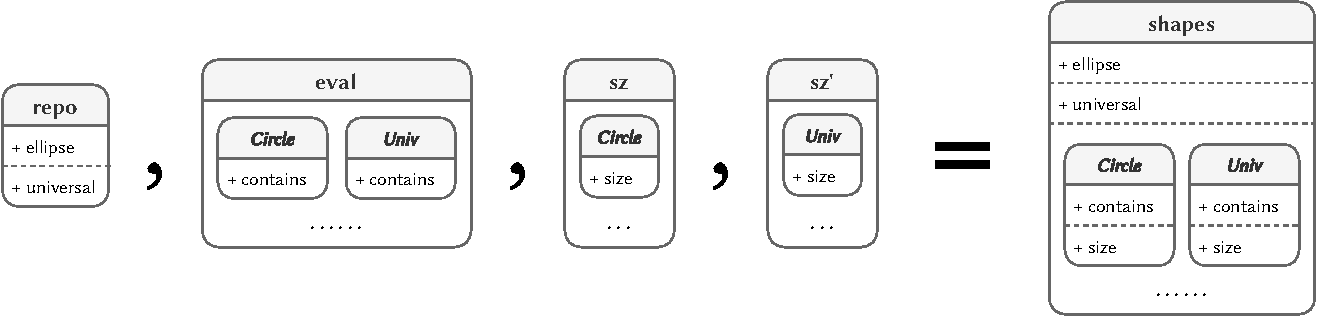
\includegraphics[width=\textwidth]{merge.pdf}
  \caption{A visualization of nested trait composition.} \label{fig:compose}
\end{figure}

\noindent
We provide the final semantic domain (\lstinline{Eval&Size}), as the type
argument, for the trait \lstinline{repo} and merge it with three other modularly
defined traits. The trait composition is called
\emph{nested}~\citep{bi2018essence} because not only different sets of
constructors, but also different semantics nested in the same constructor are
merged. In our case, both interpretations are available under the two sets of
language constructs after nested composition, as visualized in
\autoref{fig:compose}. Here, the language constructs and their semantics form a
two-level hierarchy of traits. Such composition of whole hierarchies can be
traced back to \emph{family polymorphism}~\citep{ernst2001family}. With this
powerful mechanism of nested composition, we can easily develop highly modular
\emph{product lines}~\citep{apel2013feature} of DSLs, where DSL features can be
composed \emph{à la carte}.

\subsection{Dependency Injection and Domain-Specific Optimizations} \label{sec:deps}

Now we illustrate CP's support for \emph{modular dependent interpretations}. We
skip the simpler example with \lstinline{text} and focus on the more interesting
example with \lstinline{isUniv} and \lstinline{isEmpty}. Similarly to the deep
embedding in Haskell in \autoref{sec:transform}, we define two compositional
traits \lstinline{chkUniv} and \lstinline{chkEmpty}:

\begin{lstlisting}
type IsUniv  = { isUniv:  Bool };
type IsEmpty = { isEmpty: Bool };

chkUniv = trait implements RegionSig<IsEmpty => IsUniv> => {
  (Univ         ).isUniv = true;
  (Outside     a).isUniv = a.isEmpty;
  (Union     a b).isUniv = a.isUniv || b.isUniv;
  (Intersect a b).isUniv = a.isUniv && b.isUniv;
  (Translate _ a).isUniv = a.isUniv;
  (Scale     _ a).isUniv = a.isUniv;
                _.isUniv = false;
};

chkEmpty = trait implements RegionSig<IsUniv => IsEmpty> => {
  (Empty        ).isEmpty = true;
  (Outside     a).isEmpty = a.isUniv;
  (Union     a b).isEmpty = a.isEmpty && b.isEmpty;
  (Intersect a b).isEmpty = a.isEmpty || b.isEmpty;
  (Translate _ a).isEmpty = a.isEmpty;
  (Scale     _ a).isEmpty = a.isEmpty;
                _.isEmpty = false;
};
\end{lstlisting}

\noindent
The first thing to note is that the sort of \lstinline{RegionSig} is
instantiated with two types separated by a fat arrow (\lstinline{=>}). This is
how we \emph{refine} interface types for dependency injection. For example,
\lstinline{chkUniv} does not implement \lstinline{RegionSig<IsEmpty>}, but we
assume the latter is available. The static type checker of CP guarantees that
\lstinline{chkUniv} is later merged with another trait that implements
\lstinline{RegionSig<IsEmpty>}. That is why we can safely use
\lstinline{a.isEmpty} when implementing \lstinline{(Outside a).isUniv}. The
second trait \lstinline{chkEmpty} is just the dual of \lstinline{chkUniv}. It is
hard to define such interpretations modularly in traditional approaches because
they are dependent, but we make them compositional via dependency injection.
Lastly, \lstinline{_.isUniv} and \lstinline{_.isEmpty} are \emph{default
patterns}, which compensate for the remaining constructors declared in the
interface. For example, \lstinline{_.isUniv = false} implies
\lstinline{Empty.isUniv = false} and \lstinline{Circle.isUniv = false}. Note
that in CP, for modularity, patterns are \emph{unordered}, unlike functional
languages like Haskell or ML. Therefore, default patterns are local to the
traits where they are used. These patterns can be understood as a concise way to
fill the missing cases in the local trait. 

Another thing worth noting is that dependency injection in compositional
embeddings is more modular than direct dependencies in deep embeddings because
the former does not refer to concrete implementations. For example, in the
compositional embedding above, \lstinline{chkUniv} only requires that the
dependent trait should implement the interface \lstinline{RegionSig<IsEmpty>}.
However, in the deep embedding (see \autoref{sec:mutual}), \lstinline{isUniv}
depends on the specific \lstinline{isEmpty} implementation.

\paragraph{Delegated method patterns.}
In some complicated transformations, nested pattern matching is required to
inspect smaller constructs. Nested pattern matching is not directly supported in
CP yet. However, there is a simple transformation that we can do whenever we
would like to have nested patterns:  we can delegate the inner tasks to other
methods whereby only top-level patterns are needed. We call such a technique
\emph{delegated method patterns}.

Concerning the nested pattern matching in \autoref{sec:nested}, we can implement
it with two mutually dependent methods. Since delegated method patterns are not
reused, the two methods are defined together for the sake of simplicity (but can
always be separated into two traits):

\begin{lstlisting}
type Eliminate Region = { eliminate: Region; delOutside: Region };

elim Region = trait [fself: RegionSig<Region>]
              implements RegionSig<Region => Eliminate Region> => {
  (Outside     a).eliminate = a.delOutside;
  (Union     a b).eliminate = Union a.eliminate b.eliminate;
  (Intersect a b).eliminate = Intersect a.eliminate b.eliminate;
  (Translate v a).eliminate = Translate v a.eliminate;
  (Scale     v a).eliminate = Scale v a.eliminate;
           [self].eliminate = self;

  -- delegated method patterns:
  (Outside a).delOutside = a.eliminate;
       [self].delOutside = Outside self.eliminate;
};
\end{lstlisting}

\noindent The translation from nested pattern matching to delegated method
patterns is straightforward. Our code lifts nested patterns
(\lstinline{Outside (Outside a)}) to top-level delegated patterns. In this way,
we do not change the underlying algorithm at all. This is in contrast with
approaches like tagless-final embeddings that, as discussed in
\autoref{sec:transform}, seem unable to directly support nested patterns,
requiring different algorithms to achieve the same goal. Though our approach is
not as convenient as deep embeddings, it is noteworthy that we can just write
the original algorithm \emph{modularly}.

If we add new language constructs in the future, it is easy to augment the
traits with more top-level patterns, but extending nested patterns is difficult
because there is no name to denote the \emph{extension point}. With delegated
method patterns, the method name \lstinline{delOutside} offers an extension
point for additional cases in the nested pattern matching. For instance, if we
wish for an extension supporting a new kind of region and a special case for
eliminating a region outside this kind of region
(\lstinline{eliminate (Outside (SomeRegion params))}), we can have a trait with
a method pattern of the following form, modularly defined in another trait:

\begin{lstlisting}
(SomeRegion params).delOutside = ...
\end{lstlisting}

\noindent
Although we believe that the design of CP can be improved to better support
similar logic to nested patterns, there are important differences between
traditional (closed) forms of pattern matching and open pattern
matching~\citep{zhang2020castor}. For instance, patterns in CP are unordered for
compositionality, but the order of patterns matters in conventional pattern
matching. Thus the design of improved language support for nested patterns in
CP, which could make the use of delegated method patterns more convenient,
requires further research and is left for future work.

\paragraph{Linguistic reuse after transformations.}
Before finishing the discussion of modular transformations, let us revisit CP's
support for linguistic reuse: can we still have meta-language optimizations for
free after complicated transformations? The answer is yes. To demonstrate this
point, we can modify the definition of \lstinline{circles} in
\autoref{sec:sharing} to have an inefficient
\lstinline{Outside (Outside (Circle 1.0))}. As usual, we compose all the
necessary traits together to make sure no dependencies are missing:

\begin{lstlisting}
test' = new sharing' @(Size & Eliminate Size) , sz , sz' , elim @Size;
test'.circles.eliminate.size
\end{lstlisting}

\noindent
The evaluation terminates as quickly as before, meaning that meta-language
optimizations are still performed even after a transformation.

We should remark that there are limits to the form of implicit sharing (and
linguistic reuse) that shallow embeddings or compositional embeddings provide.
For both shallow and compositional embeddings, implicit sharing will not work if
the interpretation is a function, such as \lstinline{contains}. In such cases,
the sharing is still lost. Nevertheless, implicit sharing is an important
feature that is often exploited in shallow DSLs. With compositional embeddings,
we can take this idea further and make it work even after some transformations
and optimizations have been applied. Moreover, it is also possible to adopt
solutions with explicit sharing by modeling a \lstinline{Let} construct in the
DSL.

\subsection{A Detailed Comparison between Different Embedding Approaches} \label{sec:comparison}

\begin{table}[b!]
\caption{A detailed comparison between different embedding approaches.} \label{tab:comparison}
\centering
\begin{tabular}{*{6}{c}}
\toprule
                                       &\textsc{Shallow}& \textsc{Deep} &\textsc{Hybrid}& \textsc{Poly.}& \textsc{Comp.}\\
\midrule \midrule
Transcoding free                       &    \CIRCLE     &    \CIRCLE    &    \Circle    &    \CIRCLE    &    \CIRCLE    \\
Linguistic reuse                       &    \CIRCLE     &    \Circle    &    \CIRCLE    &    \CIRCLE    &    \CIRCLE    \\
Language construct extensibility       &    \CIRCLE     &    \Circle    &\LEFTcircle$^1$&    \CIRCLE    &    \CIRCLE    \\
Interpretation extensibility           &    \Circle     &    \CIRCLE    &    \CIRCLE    &    \CIRCLE    &    \CIRCLE    \\
Transformations and optimizations      &    \Circle     &    \CIRCLE    &    \CIRCLE    &\LEFTcircle$^2$&\LEFTcircle$^2$\\
Linguistic reuse after transformations &    \em n/a     &    \Circle    &    \Circle    &    \CIRCLE    &    \CIRCLE    \\
Modular dependencies                   &    \Circle     &\LEFTcircle$^3$&\LEFTcircle$^3$&    \Circle    &    \CIRCLE    \\
Nested pattern matching                &    \Circle     &    \CIRCLE    &    \CIRCLE    &    \Circle    &\LEFTcircle$^4$\\
\bottomrule
\end{tabular}
\vskip 1ex
{\footnotesize
  $^1$ The extensibility of language constructs is limited or precludes exhaustive pattern matching.\\
  $^2$ Transformations require some ingenuity and are sometimes awkward to write.\\
  $^3$ Dependencies do not require code duplication but still refer to concrete implementations.\\
  $^4$ Nested pattern matching is implemented as delegated method patterns.\\
}
\end{table}

\noindent
In \autoref{tab:comparison}, we compare existing embedding approaches in the
literature with compositional embeddings. Shallow and deep embeddings have been
discussed in detail in \autoref{sec:embed}, and the table summarizes the points
that we have made. Hybrid
approaches~\citep{rompf2012scala,svenningsson2015combining,jovanovic2014yinyang}
employ both embeddings together. However, transcoding from shallow to deep is
generally needed, as both shallow and deep implementations must coexist side by
side. There is a clear boundary between the two parts: linguistic reuse is
available only in the shallow part, while complex transformations are available
only in the deep part. Therefore, it is still hard to exploit host-language
features after transformations. In work by
\citeauthor{svenningsson2015combining}, we cannot add more constructs to the
deeply embedded AST but can only extend shallowly embedded syntactic sugar. In
Scala, if \emph{open} case classes~\citep{emir2007matching} are used for deep
embeddings, ASTs are also extensible but do not ensure the exhaustiveness of
pattern matching. Compositional embeddings offer a unified approach directly
capable of all these functionalities.

\paragraph{Non-modular dependencies in modular embeddings.}
Polymorphic embeddings~\citep{hofer2008polymorphic}, tagless-final
embeddings~\citep{carette2009finally,kiselyov2010typed}, and object
algebras~\citep{oliveira2012extensibility} (denoted as \textsc{Poly.} in the
table) also provide a unified encoding where most advantages of shallow and deep
embeddings are available. However, they cannot deal with dependencies modularly.
Let us take tagless-final embeddings for example, which can also be implemented
in Haskell. We refer curious readers to \autoref{sec:tagless} for the complete
code.

In the tagless-final embedding, region constructors are defined in a type class
instead of a closed algebraic data type, and \lstinline{Size} can be modularly
defined as an instance of the type class since it has no dependency:

\noindent
\begin{minipage}{0.48\textwidth}
\begin{lstlisting}[language=Haskell,deletekeywords={union,intersect}]

class RegionHudak repr where
  circle    :: Double -> repr
  outside   :: repr -> repr
  union     :: repr -> repr -> repr
  intersect :: repr -> repr -> repr
  translate :: Vector -> repr -> repr
\end{lstlisting}
\end{minipage}%
\begin{minipage}{0.52\textwidth}
\begin{lstlisting}[language=Haskell,deletekeywords={union,intersect}]
newtype Size = S { size :: Int }
instance RegionHudak Size where
  circle      _ = S 1
  outside     a = S $ a.size + 1
  union     a b = S $ a.size + b.size + 1
  intersect a b = S $ a.size + b.size + 1
  translate _ a = S $ a.size + 1
\end{lstlisting}
\end{minipage}

\noindent
But how about the textual representation? As a first try, we might write:

\begin{lstlisting}[language=Haskell]
newtype Text = T { text :: String }
instance RegionHudak Text where
  circle  r = T { text = "circular region of radius " ++ show r }
  outside a = T { text = "outside a region of size " ++ show a.size }
  ......
\end{lstlisting}

\noindent
Unfortunately, we will get a type error concerning \lstinline{a.size} because
\lstinline{a} has type \lstinline{Text} and thus does not contain a field named
\lstinline{size}. Once we need operations that have some dependencies on other
operations, we get into trouble!

A simple workaround is to pack the two operations together and duplicate the
code of size calculation. We have already described this approach for shallow
embeddings in \autoref{sec:transform}, and the same workaround works for
tagless-final embeddings:

\begin{lstlisting}[language=Haskell,deletekeywords={union,intersect}]
data SizeAndText = ST { size :: Int, text :: String }
instance RegionHudak SizeAndText where
  circle  r = ST { size = 1, text = "circular region of radius " ++ show r }
  outside a = ST { size = a.size + 1
                 , text = "outside a region of size " ++ show a.size }
  ......
\end{lstlisting}

\noindent However, this is not modular since we have to duplicate code for size
calculation, even though the size calculation is completely independent of the
textual representation. If we have another operation that depends on
\lstinline{size}, we have to repeat the same code even again. This workaround is
an \emph{anti-pattern}, which violates basic principles of software engineering.
Duplicating code every time we need a dependent interpretation is a serious
problem since dependencies are extremely common. Nearly all non-trivial code
will have dependencies. In functional programming, it is common to have
functions defined by pattern matching that call other functions defined by
pattern matching, which is where an important form of dependencies appears. As
shown in \autoref{sec:fancier}, some workarounds that avoid code duplication in
Haskell are possible, but this typically comes at the cost of more code and the
use of advanced language features. 

\paragraph{The third dimension of the expression problem.}
In essence, dependencies are a third dimension that is not discussed in the
formulation of the expression problem by \citet{wadler1998expression}: whether
dependencies require code duplication or not. If we take this into
consideration, we can get a revised formulation of the expression problem, where
instead of only two dimensions, we have a third dimension that evaluates the
ability of an approach to deal with dependencies. With this extra dimension
taken into account, what we get is \autoref{tab:3d}. While tagless-final or
other embeddings address the two original dimensions of extensibility modularly,
they become non-modular with respect to dependencies, and programming with
dependencies becomes significantly more awkward compared to conventional FP or
OOP.

\begin{table}[b]
\caption{A briefer comparison regarding the three dimensions of the expression problem.} \label{tab:3d}
\centering
\begin{tabular}{*{5}{c}}
\toprule
                    &     FP  &     OOP &\textsc{Poly.}&\textsc{Comp.}\\
\midrule \midrule
New constructs      & \Circle & \CIRCLE &      \CIRCLE &      \CIRCLE \\
New functions       & \CIRCLE & \Circle &      \CIRCLE &      \CIRCLE \\
\emph{Dependencies} & \CIRCLE & \CIRCLE &      \Circle &      \CIRCLE \\
\bottomrule
\end{tabular}
\vskip 1ex
{\footnotesize \CIRCLE \; no code duplication \qquad
               \Circle \; code duplication needed}
\end{table}

Note that we are not the first to observe the problem with dependencies. The
problem above is known and discussed widely in the literature. In the context of
polymorphic embeddings, \citet{hofer2008polymorphic} face the problem of
dependencies and use the non-modular approach with tuples. Later
\citet{hofer2010modular} adopt an extensible visitor pattern to improve
modularity, but this results in much more boilerplate code. In his lecture notes
on tagless-final interpreters, \citet{kiselyov2010typed} has a strong focus on
discussing how to write non-compositional interpretations, which basically
include operations with dependencies and nested pattern matching. He shows that
non-compositional programs can often be rewritten as programs that use contexts
instead. The problem of modular dependencies has been widely discussed within
the context of object algebras. Most recently,
\citet{zhang2017evf,zhang2020castor} propose solutions to the problem using
meta-programming techniques. \citet{zhang2019shallow} further explore modular
solutions in both Scala and Haskell, but their approaches still require a lot of
boilerplate code. In Scala, it is due to a lack of language support for nested
composition, whereas Haskell needs to encode dependencies via type classes to
modularize dependent interpretations (see \autoref{sec:fancier} for a similar
solution). The drawbacks of the existing solutions above motivate the design of
CP and compositional embeddings.

\paragraph{Transformations.}
It is widely believed that transformations and optimizations are much easier to
write in deep embeddings~\citep{jovanovic2014yinyang,scherr2014implicit}. We
agree that it requires some ingenuity and is sometimes awkward to write complex
transformations in compositional embeddings, but \citet{kiselyov2010typed} has
demonstrated that several challenging transformations can be written with
tagless-final embeddings. Compositional programming is a generalization of such
forms of embeddings, and therefore all the transformations are possible with
tagless-final embeddings are also possible in CP. Even for structurally
non-local transformations, we can instantiate a sort with a function type (e.g.
\lstinline{RegionSig<Ctx->Region>}) and pass down the context when traversing
the AST. Such contextual transformations can also be modular with the help of
\emph{polymorphic contexts}~\citep{zhang2021compositional}. We have implemented
an example of common subexpression elimination inspired by
\citet{kiselyov2011implementing} (which can be found in our online
implementation). Both our code and \citeauthor{kiselyov2011implementing}'s are
not fully modular with respect to an auxiliary data structure (his
implementation relies on a closed algebraic data type). In our case, this is
because nested composition for recursive types is currently not supported, which
relies on future theoretical progress of reconciling distributive subtyping and
recursive types. Nevertheless, our approach is less entangled than tagless final
embeddings since we can handle dependent transformations modularly.

\section{\ExT: A DSL for Document Authoring} \label{sec:dsl}

We have presented the advantages of compositional embeddings using a relatively
small DSL. One may wonder if our approach scales to larger DSLs. As our answer
to this question, we developed a larger DSL for document authoring called \ExT.

\ExT applies compositional embeddings to a document DSL, inspired by \LaTeX{}
and Scribble~\citep{flatt2009scribble}. We have also done minor syntactic
extensions to the CP language to support writing documents more naturally. Since
documents usually involve large portions of text, it would be awkward to write
such portions of text using string literals adopted by most programming
languages. CP does not yet have facilities for syntactic extension that other
languages (e.g. Racket, Haskell, or Coq) offer, so we have extended the parser
directly. Thus, CP parses some document-specific syntax and desugars it to
compositionally embedded fragments during parsing. Such a generative approach is
similar to Racket macros~\citep{ballantyne2020macros} and Template
Haskell~\citep{sheard2002template}, which provide more flexible facilities for
performing such desugaring. Nevertheless, the surface syntax of \ExT is
essentially a set of lightweight syntactic sugar for its underlying
compositional embeddings (similar, for instance, to Scribble in Racket).

\subsection{Design Goals and Non-Goals} \label{sec:goals}

There are already a large number of document DSLs, so why shall we create yet
another one? We explain why by identifying important design goals and non-goals
of \ExT.

\paragraph{A document language for the web.}
A first goal is to have a lightweight but powerful document language tailored
mostly for the web. We view \ExT as an alternative to Wikitext~\citep{wikitext},
the markup language used by Wikipedia, which shares similar goals. Similar to
Wikipedia pages, users can directly edit \ExT documents on a web page. But
different from Parsoid~\citep{parsoid}, the official Wikitext parser that runs
on the server side, our implementation can directly render documents on the
browser side.

\paragraph{General-purpose computation.}
The majority of existing document DSLs (e.g. CommonMark~\citep{mark},
Textile~\citep{textile}, and reStructuredText~\citep{rst}) have a fixed set of
language features and do not provide general-purpose computation. For instance,
we may want to compute a table from some data, like a table listing the largest
cities in descending order of population. For such kinds of tasks, it is useful
to have mechanisms for general-purpose computation that allow us to
\emph{compute} documents rather than manually write them.

Although some other document DSLs provide language constructs that enable some
computation, they still have significant limitations. For instance, Wikitext
provides templates, which play a role similar to functions in conventional
programming languages. However, templates cannot perform arbitrary computation
as CP does. The documentation says,\footnote{The sentence is extracted from
\url{https://en.wikipedia.org/wiki/Wikipedia:TEMPLATE_LOOP}.} ``A template can
call itself but will stop after one iteration to prevent an infinite loop.'' In
other words, templates by themselves are incapable of recursion or loops, but in
practice, loops are often needed in Wikipedia. For instance,
\lstinline|{{loop}}| has been used on approximately 99,000 pages.\footnote{The
number of transclusions (99,000 as of July 2022) is shown at
\url{https://en.wikipedia.org/wiki/Template:Loop}.} A Lua extension was
introduced to bypass such restrictions, and the widely-used template
\lstinline|{{loop}}| invokes \lstinline{string.rep} in Lua. Instead of handing
it over to an external language, CP directly supports functions, and thus
general-purpose computation is easily done in \ExT, including recursion. 

\paragraph{Static type checking.}
In contrast to many document languages, CP and \ExT are statically type checked.
Static type checking enables us to detect some errors that may arise when
processing documents. In applications like wikis, it is very frequent that we
need some form of structured data. States or cities, for example, may have
infoboxes associated with them that list several pieces of data, such as areas,
populations, official languages, etc. Using simple text to store such data can
easily lead to simple errors. In addition, if we want to enable computed
information as previously described, then it is useful to have a type system
that allows us to write functions that take a well-defined form of structured
data. Most document languages that we know of, including Wikitext, \LaTeX{}, and
Scribble, are not statically typed. We will discuss some examples where static
typing is helpful in \ExT in \autoref{sec:typing}.

\paragraph{Extensible meta-programming and customizability.}
A benefit of modeling a DSL as an algebraic data type or a compositional
interface is that we can easily write meta-functions over the abstract syntax of
the DSL. For instance, in the context of documents, such meta-functions could
include rendering to various backends (such as \LaTeX{} or HTML) or computing a
table of contents based on the document tree. In many external DSLs, such
meta-functions are typically much harder to write, requiring us to directly
modify the implementation. However, by embedding a DSL, the host language can
act as a meta-language for the DSL and allow us to easily write meta-programs,
for instance, as functions to process the AST by pattern matching.

In addition, the extensibility of compositional embeddings enables a form of
extensible meta-programming: not only can we write meta-functions, but those
meta-functions can be extended later to cater for new language constructs
modularly defined by users. This enables DSL users to \emph{modularly} extend
the basic document language to add their own extensions, including infoboxes,
vector graphics, etc. While Scribble does provide good facilities for syntactic
extension and meta-programs, the document structure is fixed~\citep{scribble},
so the DSL is not fully extensible. In short, \ExT is designed to be extensible
and highly customizable by users. 

\paragraph{Non-goals.}
Currently, our implementation of CP is a fairly naive call-by-need interpreter,
so the performance of \ExT is not competitive with well-established tools like
\LaTeX. Furthermore, unlike \LaTeX, which has extensive libraries developed over
many years, there are no third-party libraries for \ExT. Thus, \ExT is
\emph{not} yet production-ready. Another non-goal is security. Since we never
sanitize user-generated HTML, it is easy to perform JavaScript code injection on
our website. It is off-topic to consider how to ensure web security here.

\subsection{Syntax Overview}

\begin{figure}
\begin{subfigure}{0.58\textwidth}
\begin{Verbatim}[fontsize=\small]
\Section[
  Welcome to
  \Href("https://plground.org")[PLGround]!
]
\Bold[CP] is a \Emph[compositional]
programming language. \\\\
There are \(1+1+1+1) key concepts in CP:
\Itemize[
  \Item[Compositional interfaces;]
  \Item[Compositional traits;]
  \Item[Method patterns;]
  \Item[Nested trait composition.]
]
\end{Verbatim}
\caption{\ExT code.}
\end{subfigure}%
\begin{subfigure}{0.42\textwidth}
\scalebox{0.8}{\begin{minipage}{\textwidth}
\section*{%
  Welcome to
  \href{https://plground.org}{PLGround}!
}
\textbf{CP} is a \emph{compositional}
programming language. \\\\
There are 4 key concepts in CP:
\begin{itemize}
\item Compositional interfaces;
\item Compositional traits;
\item Method patterns;
\item Nested trait composition.
\end{itemize}
\end{minipage}}
\vspace{1em}
\caption{Rendered document.}
\end{subfigure}
\caption{A sample document illustrating \ExT syntax.} \label{fig:example}
\end{figure}

\noindent
The syntax of \ExT is designed for easy document authoring, as shown in
\autoref{fig:example}. It is reminiscent of \LaTeX, but still has significant
differences. The similarity is that plain text can be directly written while
commands start with a backslash. But we choose different brackets for command
arguments:

\begin{itemize}
\item \Verb|\Cmd[...]| encloses document arguments. Square brackets indicate
      that a sequence of nested elements is recursively parsed. (Most commands
      in \autoref{fig:example} are in such a form, for example,
      \lstinline|\Section| and \lstinline|\Bold|.)
\item \Verb|\Cmd(...)| encloses positional arguments. Parentheses indicate that
      the whole construct is desugared to function application.
      (\lstinline|\Href| in \autoref{fig:example} is an example.)
\item \Verb|\Cmd{...}| encloses labeled arguments. Braces indicate that these
      arguments are wrapped in a record. (As mentioned in \autoref{sec:typing},
      \lstinline|\Line{ x1 = 0.0; y1 = 0.0; x2 = 4.6; y2 = 4.8 }| uses this form
      to distinguish different attributes.)
\end{itemize}

\noindent
A command can be followed by an arbitrary number of different arguments in any
order. This syntax is more flexible than the fixed form
\lstinline|@op[...]{...}| in Scribble. Although both arguments are optional in
Scribble, they can neither occur more than once nor be shuffled. In addition,
there are two more useful \ExT constructs. One is string interpolation with the
form \lstinline{\(...)}, which has exactly the same syntax as the Swift
programming language. We can see an example of string interpolation in
\autoref{fig:example}: \lstinline|\(1+1+1+1)|. It will be desugared to
\lstinline{Str (toString (1+1+1+1))}. This example will execute the code, which
computes ``4'', and its string form will be interpolated in the document. The
other construct is double backslashes (\lstinline{\\}), a shorthand for newline,
which is borrowed from \LaTeX. In \ExT, it is equivalent to the
\lstinline{\Endl} command. There is also an example in \autoref{fig:example},
which inserts a newline character between the first and second sentences in the
body. 

\paragraph{Desugaring.}
As mentioned earlier, all \ExT constructs are desugared to normal CP code. For
example, the following two expressions are equivalent (the document DSL is
enclosed within backticks):

\begin{lstlisting}
`\Entry("id"){ hidden = true; level = 1 }[This entry is \Emph[hidden]]`
-- is desugared to:
Entry "id" { hidden = true; level = 1 } (Comp (Str "This entry is ")
                                              (Emph (Str "hidden")))
\end{lstlisting}

\noindent Here, \lstinline{Comp} and \lstinline{Str} are two special commands
that are assumed to be implemented by library authors. \lstinline{Comp} is used
for composing an AST of document elements, while \lstinline{Str} is for plain
text.

\paragraph{Specification.}
The grammar of \ExT can be summarized in whole as follows (\lstinline{<arg>*}
means that \lstinline{<arg>} may occur zero or more times):

\begin{Verbatim}[fontsize=\small]
<doc> ::= <str> | "\" <esc>
<esc> ::= <cmd> <arg>* | "(" <exp> ")" | "\"
<arg> ::= "[" <doc> "]" | "(" <exp> ")" | "{" <rcd> "}"

<str> ::= text without "\" and "]"
<cmd> ::= identifier
<exp> ::= expression
<rcd> ::= record fields
\end{Verbatim}

\subsection{Extensible Commands with Multi-Backend Semantics}

\ExT is so flexible that only a few commands are really compulsory. Additional
commands and their semantics can be extended as needed. At the very beginning,
we only need to define the aforementioned three special commands:

\begin{lstlisting}
type DocSig<Element> = {
  Comp: Element -> Element -> Element;
  Str:  String -> Element;
  Endl: Element;
};
\end{lstlisting}

\noindent
However, for rich text in real-world documentation, these commands are not
sufficient for various document elements. Adding new commands and their
semantics is not hard at all in compositional embeddings, like what we have done
in \autoref{sec:syntax} and \autoref{sec:semantics}. Language interfaces can be
separately declared and then intersected with each other. Besides extensible
commands, their semantics are also retargetable. We can modularly create
different traits for different backends, such as HTML and \LaTeX:

\begin{lstlisting}
type HTML = { html: String };
html = trait implements DocSig<HTML> => {
  (Comp l r).html = l.html ++ r.html;
  (Str    s).html = s;
  (Endl    ).html = "<br>";
};

type LaTeX = { latex: String };
latex = trait implements DocSig<LaTeX> => {
  (Comp l r).latex = l.latex ++ r.latex;
  (Str    s).latex = s;
  (Endl    ).latex = "\\\\";
};
\end{lstlisting}

\begin{figure}
  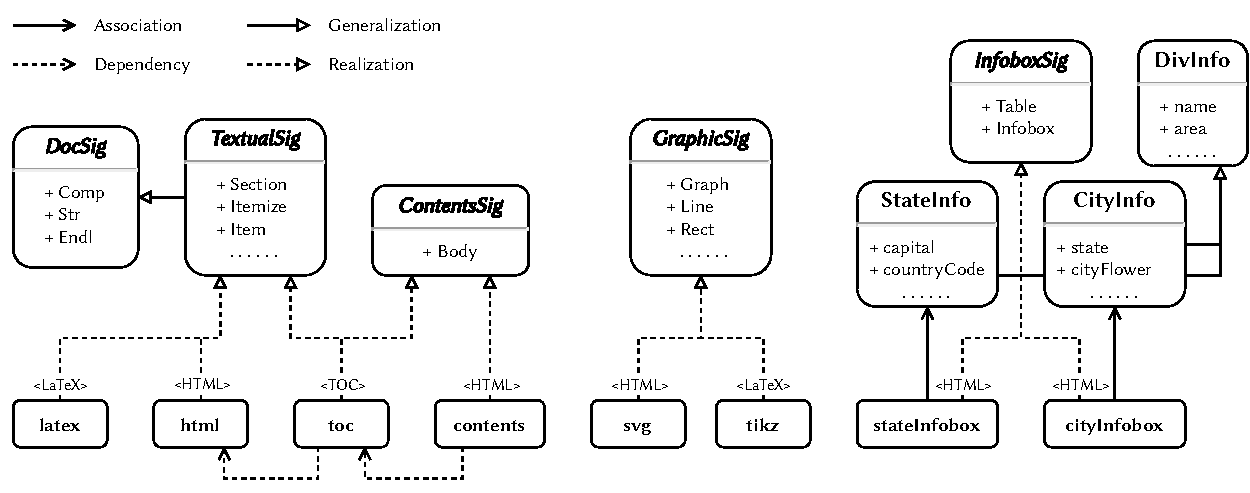
\includegraphics[width=\textwidth]{libraries.pdf}
  \caption{A simplified diagram of \ExT components.} \label{fig:diagram}
\end{figure}

\paragraph{The components of \ExT.}
We have implemented several extensions of \ExT, as shown in
\autoref{fig:diagram}. In the upper part of the diagram, the capitalized names
in a bold italic font (e.g. {\small \sffamily \bfseries \itshape DocSig}) are
compositional interfaces, while those in a bold upright font (e.g. {\small
\sffamily \bfseries DivInfo}) are normal types. The smaller boxes at the bottom
of the diagram are compositional traits. They implement different interfaces
with the sorts specified on the dashed arrows, (e.g. {\small \sffamily <HTML>}).
Specifically, \lstinline{TextualSig} adds a set of common commands for rich
text, such as \lstinline{Section}, \lstinline{Itemize}, \lstinline{Item}, etc.
It extends \lstinline{DocSig} and targets both HTML and \LaTeX.
\lstinline{GraphicSig} is used to draw vector graphics (including lines,
rectangles, circles, etc.), which are supported in HTML and \LaTeX{} via SVG and
Ti\emph{k}Z respectively. \lstinline{InfoboxSig} targets only HTML and adds
Wikipedia-like infoboxes (containing, for instance, information about areas and
populations of states or cities). All these compositional interfaces and traits
can be combined to form a heterogeneous composition. Notably, the implementation
of \lstinline{ContentsSig}, which is used to generate a table of contents,
introduces some non-trivial dependencies (see \autoref{sec:minipedia}).

\subsection{Static Typing} \label{sec:typing}

A major difference of \ExT from other document DSLs is that it is statically
type checked. With static typing, potential type errors can be detected ahead of
time, saving users' time for debugging. For example, when drawing a line using
SVG, we need to use the \lstinline{<line>} element with four numeric coordinates
(\lstinline{x1}, \lstinline{y1}, \lstinline{x2}, and \lstinline{y2}). However,
since additional information of an SVG element is represented as XML attributes,
all of the coordinates have to be quoted as strings instead of numbers. Only
after rendering it with a web browser and opening developer tools can one check
if attributes are valid. In \ExT, we model the line construct like this:

\begin{lstlisting}
type GraphicSig<Graphic> = {
  Line: { x1: Int; y1: Int; x2: Int; y2: Int } -> Graphic;
  -- and more constructors
};
\end{lstlisting}

\noindent
Before rendering lines via SVG, the types of arguments are checked against the
language interface, and invalid values are rejected in advance. Note that the
error messages are reported in terms of the \ExT surface syntax, which is more
friendly to users than some meta-programming techniques, where errors are
reported in terms of the generated code.

When modeling infoboxes and bibliography in \autoref{sec:minipedia}, we also
make use of data types to represent structured information. For example, we use
\lstinline{DivInfo} to model common information required by all political
divisions, as well as two specific types for states and cities respectively,
which extend \lstinline{DivInfo} using intersection types:

\noindent
\begin{minipage}{0.28\textwidth}
\begin{lstlisting}
type DivInfo = {
  name:       String;
  area:       Int;
  population: Int;
  languages: [String];
};
\end{lstlisting}
\end{minipage}
\hfill
\begin{minipage}{0.29\textwidth}
\begin{lstlisting}
type StateInfo =
       DivInfo & {
  countryCode: String;
  religions:  [String];
  -- and more fields
};
\end{lstlisting}
\end{minipage}
\hfill
\begin{minipage}{0.27\textwidth}
\begin{lstlisting}
type CityInfo =
      DivInfo & {
  cityFlower: String;
  timeZone:   String;
  -- and more fields
};
\end{lstlisting}
\end{minipage}

\noindent In this case, there is quite a bit of structure in the data. It
statically describes what fields are allowed and what types these fields have. 

\section{Evaluation of Compositionally Embedded \ExT}

In this section, we describe three applications of CP, compare them with
alternatives in other document languages, and evaluate the use of
compositionally embedded \ExT for the three applications.

\subsection{Minipedia} \label{sec:minipedia}

Minipedia is a mini document repository of states and cities, which reconstructs
a small portion of Wikipedia. Minipedia currently contains pages of the world's
ten smallest countries and their capitals, as well as a structured data file
storing all facts about them used for infoboxes. There are also pages consisting
of sorted tables of microstates by area or population, which are computed using
the information stored in the data file. Minipedia comprises over 4,000 lines of
code in total, most of which is accounted for by document pages. Among the rest,
the data file and \ExT libraries account for around 300 and 200 lines of code,
respectively.

\paragraph{Drawbacks of Wikipedia.}
Compared to our approach, Wikipedia and its markup language Wikitext have
several drawbacks, as partly mentioned in \autoref{sec:goals}:
\begin{itemize}
\item All data in Wikitext is in string format. Wikitext does not differentiate
      data types like \lstinline{Int}, \lstinline{Bool}, etc. This makes type
      errors remain uncaught in Wikipedia infoboxes. For example, in the infobox
      of a country, the population field can be changed to a non-numeric
      meaningless value, and Wikipedia will not warn the editor at all.
\item Statistical data is manually written on every Wikipedia page. This can
      easily result in data inconsistency for the same field across different
      pages, and even for different places on the same page. For example, the
      population size on a country page is often different from that in a
      statistical page listing all countries by population, owing to different
      data sources.
\item Wikitext provides user-defined templates as a reusable unit of document
      fragments. They can be parametrized and play a similar role to functions.
      However, they do not natively support general-purpose computation like
      recursion. Along with the Lua extension and parser functions, Wikitext
      offers some computational power to Wikipedia documents, but it is not as
      easy to use as \ExT is.
\end{itemize}

\paragraph{Type safety and data consistency.}
Minipedia has a structured data file containing the information of states and
cities, each piece of which is modeled as a record. The record types have been
shown in \autoref{sec:typing}. Every record for states or cities is type checked
against their corresponding types and collected in two arrays in the data file:

\noindent
\begin{minipage}{0.5\textwidth}
\begin{lstlisting}
tuvalu = {
  name       = "Tuvalu";
  area       = 26;
  population = 10645;
  -- and more fields
} : StateInfo;
states = [tuvalu; {- and more -}];
\end{lstlisting}
\end{minipage}%
\begin{minipage}{0.5\textwidth}
\begin{lstlisting}
funafuti = {
  name       = "Funafuti";
  area       = 2;
  population = 6320;
  -- and more fields
} : CityInfo;
cities = [funafuti; {- and more -}];
\end{lstlisting}
\end{minipage}
\smallskip

\noindent Such a centralized data file forces different documents to read from
the same data source and prevents data inconsistency. Not only infoboxes but
also computed documents like sorted lists of countries can be created using the
information from the data file. Moreover, if the area of Tuvalu, for example, is
assigned a string value, there will be a type error before rendering.

\paragraph{Writing Minipedia pages in \ExT.}
Writing Minipedia documents is enabled by the \ExT libraries shown in
\autoref{fig:diagram}. Different features of \ExT are defined in different
libraries, and we can import whatever libraries we want when writing a document.
For Minipedia, we only need HTML-related libraries. There are two modes for
document authoring in Minipedia: ``doc-only'' and ``program''. In the
``doc-only'' mode, with required libraries specified, documents are written
directly in \ExT without any wrapping code in CP, as shown in
\autoref{fig:example}. In the ``program'' mode, a document is created
programmatically in a mixture of CP and \ExT code. This mode makes
general-purpose computation easier to write in a document.

For example, a sorted table of the smallest countries by area demonstrates
general-purpose computation in the ``program'' mode. The program begins with an
\lstinline{open} directive, which imports definitions from the specified
libraries. We sort the array of countries imported from \lstinline{Database}
using a predefined function \lstinline{sort} and then iterate it to generate
\ExT code. As explained in \autoref{sec:sharing}, we use self-type annotations
to inject dependencies on the library commands. The intersection type
\lstinline{DocSig<T>&TableSig<T>} allows \ExT commands from both compositional
interfaces to be used in the trait \lstinline{doc}:

\begin{lstlisting}
open LibDoc;
open LibTable;
open Database;

sortedStates = sort states;
doc T = trait [self: DocSig<T>&TableSig<T>] => {
  table = letrec rows (i: Int): T = if i == 0 then `\Trow[
      \Theader[No.]   \Theader[Country]      \Theader[Area (km^2)]
    ]` else let state = sortedStates!!(i-1) in `\rows(i-1) \Trow[
      \Tdata[\(i+1)]  \Tdata[\(state.name)]  \Tdata[\(state.area)]
    ]` in `\Tbody[ \rows(#sortedStates) ]`;
};
document = new doc @HTML , html , table;
document.table.html
\end{lstlisting}

\paragraph{Adding a table of contents (TOC).}
We have introduced how to write Minipedia pages using \ExT libraries, but now
let us go back and see how we implement a \ExT library. The library of TOC adds
a new command \lstinline{\Body[...]}, which prepends a TOC to the document body.
The difficulty here is that HTML rendering depends on the TOC, whereas the TOC
in turn depends on the HTML rendering of section (and sub$^n$section) titles. As
we have demonstrated in \autoref{sec:deps}, we can modularly tackle such complex
dependencies by refining the interface types:

\begin{lstlisting}
type ContentsSig<Element> = { Body: Element -> Element };
type TOC = { toc: String };

contents = trait implements ContentsSig<TOC => HTML> => {
  [self]@(Body e).html = self.toc ++ e.html;
};
toc = trait implements TextualSig<HTML => TOC> & ContentsSig<TOC> => {
  (Comp        l r).toc = l.toc ++ r.toc;
  (Section       e).toc = listItem 0 e.html;
  (SubSection    e).toc = listItem 1 e.html;
  (SubSubSection e).toc = listItem 2 e.html;
  (Body          e).toc = "<ul>" ++ e.toc ++ "</ul>";
                  _.toc = "";
};
\end{lstlisting}

\noindent With \lstinline{TOC} specified in \lstinline{ContentsSig<TOC => HTML>}
and the self-reference specified in \lstinline{[self]}, we can call
\lstinline{self.toc} to generate a TOC when rendering HTML. Similarly, we can
call \lstinline{e.html} when generating the TOC since the interface type is
refined. A minor remark is that \lstinline{listItem} is an auxiliary function to
generate an appropriate \lstinline{<li>} wrapping for a given nesting level.

\subsection{Fractals and Sharing}

In the second application, we briefly introduce how to implement computational
graphics like fractals in \ExT with the help of linguistic reuse. Fractal
drawing is all about repeating the same pattern. This drives us to exploit
meta-language sharing to avoid redundant computation. We have implemented
several well-known fractals, such as the Koch snowflake, the T-square, and the
Sierpiński carpet. For the sake of simplicity, we take the Sierpiński carpet as
an example:

\begin{lstlisting}
fractal T C = trait [self: DocSig<T> & GraphicSig<T><C> & ColorSig<C> & Draw T C] implements Draw T C => {
  draw {..} =
    let center = Rect { x = x + width/3; y = y + height/3;
                        width = width/3; height = height/3; color = White } in
    if level == 0 then center else
      let w = width/3 in let h = height/3 in let l = level-1 in
      let shared = draw { x = x; y = y; width = w; height = h; level = l } in
      `\Group(id)[
         \shared
           \Translate{x=w;y=0}(shared)
             \Translate{x=2*w;y=0}(shared)
         \Translate{x=0;y=h}(shared)
           \center
             \Translate{x=2*w;y=h}(shared)
         \Translate{x=0;y=2*h}(shared)
           \Translate{x=w;y=2*h}(shared)
             \Translate{x=2*w;y=2*h}(shared)
      ]`
};
\end{lstlisting}

\noindent We make variables shared via the \lstinline{let} expressions in CP.
There are many uses in the code above but, among them, \lstinline{shared}
accelerates fractal generation the most. The variable \lstinline{shared} is
later used eight times to constitute the repeating patterns in the Sierpiński
carpet. \lstinline{\Translate} is a command declared in \lstinline{GraphicSig}
for geometric translations. With automatic linguistic reuse in \ExT, we only
need to generate a pattern once instead of repeating it eight times. Besides the
efficiency in generating fractals, our implementation of \lstinline{\Translate}
makes use of the \lstinline{<use>} element in SVG to avoid the exponential
growth of output. Therefore, the duplication of SVG elements is also eliminated.
These optimizations are available for free thanks to the linguistic reuse in
compositional embeddings.

\subsection{Customizing Charts} \label{sec:charts}

In the last application, we illustrate how line charts and bar charts are
modularly rendered using external data. Charts can be rendered into a document
using the \ExT language and its support for vector graphics. What is interesting
about charts is that there are many alternative ways to present charts and
customize them. The flexibility of the CP language, in terms of modularity and
compositionality, is then very useful here. We will show how to adapt
traditional object-oriented design patterns for compositional embeddings when
modeling graphic components.

\paragraph{Charting stocks.}
Taking stock prices as an example, we have a separate file containing data from
big companies, as well as a few configuration items for chart rendering. The
configuration includes the choice between lines and bars, whether to show
borders or legends, what labels to display, and so on. Serving as an
infrastructure, a base chart is created with the drawing functions for the
caption and axes:

\begin{lstlisting}
type Base = { caption: HTML; xAxis: HTML; yAxis: HTML };
baseChart (data: [Data]) = trait implements Base => {
  caption = `...`;  xAxis = `...`;  yAxis = `...`;
};
\end{lstlisting}

\noindent
The simplified code above shows a rough sketch, where a base trait takes data as
its parameter and implements the base interface. However, it does not implement
the primary rendering function. As we have two options to visualize stock
prices, we leave the choice to the \textsc{Strategy}
pattern~\citep{gamma1995design}.

\paragraph{\textsc{Strategy} pattern.}
Since the configuration is unknown until run time, the rendering strategy cannot
be hard-coded in the base trait. Instead, we define two strategy traits
implementing the rendering, respectively for lines and bars. They constitute two
variants of the base chart. It is not the programmer but the configurator that
decides which variant of charts should be rendered. In the original
\textsc{Strategy} pattern, a chart object delegates to a desired strategy
object, to which its mutable field points. That mutable field can be changed
from clients who use the chart. In CP, we just need to merge the base trait with
the strategy we want, without the need for mutable references:

\begin{lstlisting}
type Render = { render: HTML };
lineStrategy = trait [self: Base] implements Render => {
  render = let lines = ... in `\xAxis \yAxis \lines \caption`
};
barStrategy = trait [self: Base] implements Render => {
  render = let bars = ... in `\xAxis \yAxis \bars \caption`
};
chart = baseChart data , if config.line then lineStrategy else barStrategy;
\end{lstlisting}

\noindent
After merging, \lstinline{chart} is still a \emph{reusable trait}. This is
impossible in traditional object-oriented languages, like Java, because they
lack a dynamic way to compose classes at run time. In contrast, such a dynamic
trait composition is ubiquitous in CP. It is also easy to add a new strategy,
like switching to pie charts, and merge the base trait with the new one instead.
If a client forgets to pick any strategy, the type checker will notify them
because the trait types before and after merging are different. Moreover,
another advantage of our approach over the original strategy pattern is that the
self-type annotations make methods in the base trait accessible to strategy
traits. So \lstinline{caption}, \lstinline{xAxis} and \lstinline{yAxis} are
directly shared with strategies, requiring no extra effort to pass them as
arguments when delegating. This remedies the ``communication overhead between
Strategy and Context'' caused by the original \textsc{Strategy}
pattern~\citep{gamma1995design}.

\paragraph{\textsc{Decorator} pattern.}
Besides the \textsc{Strategy} pattern, the \textsc{Decorator}
pattern~\citep{gamma1995design} is also adapted for CP. Since decorations are
also determined by external configuration at run time, we need a modular way to
add additional drawing processes to the chart trait dynamically. When multiple
decorators are enabled, their functionalities should be added. In the original
\textsc{Decorator} pattern, the decorator class should inherit the chart class
and be instantiated with a reference to a chart object. The decorator will store
the chart object as a field and forward all methods to it. In concrete
decorators, the rendering function will be overridden to add decorations. The
decorator pattern sounds complicated in traditional object-oriented programming,
but the same goal can be achieved easily in CP using the \emph{dynamic
inheritance} provided by CP:

\begin{lstlisting}
type Chart = Base & Render;
borderDecorator (chart: Trait<Chart>) = trait [self: Chart] implements Chart inherits chart => {
  override render = let sr = super.render in let border = ... in `\sr \border`
};
legendDecorator (chart: Trait<Chart>) = trait [self: Chart] implements Chart inherits chart => {
  override caption = let legends = ... in `\legends`
};
chart' = if config.border then borderDecorator chart else chart;
chart'' = if config.legend then legendDecorator chart' else chart';
\end{lstlisting}

\noindent
A decorator takes a chart trait as the argument and creates another trait
inheriting it dynamically. In the implementation, we can override any methods as
usual, and static type safety is still guaranteed. It is worth noting that, in
\lstinline{legendDecorator}, only \lstinline{caption} is overridden while
\lstinline{render} is just inherited. In the original \textsc{Decorator}
pattern, \lstinline{render} will never be conscious of the overridden
\lstinline{caption} since the decorator hands over control to \lstinline{chart}
after forwarding \lstinline{render}. This is partly why \citet{gamma1995design}
warn readers that ``a decorator and its component aren't identical''. However,
in CP, \lstinline{chart.render} can access the overridden \lstinline{caption}
through the late-bound self-reference. This solution makes our code clean and
easy to maintain.

\paragraph{True delegation via trait composition.}
The chart application shows how other aspects of the modularity of CP are
helpful to create highly customizable DSLs. We have shown how CP adapts and
simplifies object-oriented design patterns. In general, we avoid complicated
class hierarchies in the original versions and replace them with relatively
simple trait composition. It showcases that we can get rid of verbose design
patterns if a proper language feature fills in the gap. In both patterns,
component adaptation is needed at run time, so delegation is at the heart of the
challenges.


\chapter{Type-Safe Dynamic Inheritance} \label{ch:inheritance}

This chapter presents the second case study of compositional programming:
type-safe dynamic inheritance. While dynamic inheritance is supported by many
dynamically typed languages, such as JavaScript, it poses significant challenges
for statically typed languages to implement it in a type-safe manner.
\autoref{sec:introduction} starts with a manifesto of our proposal based on a
trait model with merging. Then in \autoref{sec:background}, we show some
concrete examples in TypeScript, which extends JavaScript with static typing,
revealing type-safety issues. Finally in \autoref{sec:overview}, we show how CP
solves these issues. In short, CP supports dynamic multiple inheritance and
family polymorphism while preserving type safety.

\section{First-Class Traits with Merging} \label{sec:introduction}

Many programming language constructs are first-class. First-class functions are
a key construct of functional programming. Similarly, objects are first-class in
object-oriented programming (OOP). First-class constructs enable the
corresponding values to be abstracted by variables, passed as arguments, or
returned by functions or methods.

While classes are pervasive in most OOP languages, first-class classes are
\emph{much less} studied, and they are \emph{rarely} supported in mainstream
statically typed OOP languages. Languages such as Java, C\#, and Swift, just to
name a few, do not support first-class classes. In these languages, no variables
can abstract over classes, and thus a class cannot pick which class to inherit
from at run time. Nevertheless, some dynamically typed languages treat classes
as first-class constructs and allow dynamic inheritance. Taking
JavaScript\footnote{Although object-orientation in JavaScript is originally
prototype-based, newer standards (ECMAScript 6+) also support classes on top of
prototypes.} as an example, a base class can be passed as an argument, and the
inheritance hierarchy is determined at run time, after the application of the
function happens:
\begin{lstlisting}[language=TypeScript]
function Mixin(Base) {
  return class extends Base {
    greet() { alert('Hello, world!') }
  };
}
\end{lstlisting}
First-class classes offer powerful and flexible abstraction mechanisms for
programmers. For instance, \emph{mixins}~\citep{bracha1990mixin}, which are
class-like abstractions that can be mixed into other classes to add new
features, are encodable via first-class classes and dynamic inheritance. In our
example, the \lstinline{Mixin} function creates a class that inherits from
\lstinline{Base} and adds a \lstinline{greet} method. At run time, we can apply
\lstinline{Mixin} to different base classes that need \lstinline{greet}. Dynamic
inheritance rejects the common assumption that inheritance hierarchies are fixed
at compile time, providing a greater degree of flexibility compared to static
inheritance. Furthermore, first-class classes provide natural support for
\emph{nested classes}: classes defined within another class, or even inside
methods or functions as in the \lstinline{Mixin} example. Nested classes can
access definitions and methods in the surrounding lexical scope. In JavaScript,
nested classes are supported via first-class classes. Some other OOP languages,
such as Java, support nested classes without supporting first-class classes.

\begin{figure}
\centering
\begin{subfigure}{.33\textwidth}
\begin{lstlisting}[language=TypeScript]
class A {
  m() { return 48 }
}
\end{lstlisting}
\end{subfigure}
\begin{subfigure}{.33\textwidth}
\begin{lstlisting}[language=TypeScript]
class B extends A {
  m() { return "Hi" }
}
\end{lstlisting}
\end{subfigure}
\caption{JavaScript allows unconstrained overriding, whereas TypeScript's type
  system attempts to prevent type-unsafe overriding and statically rejects the
  example.} \label{fig:override}
\end{figure}

To ensure type-safe inheritance, an important concern is how to deal with
\emph{overriding} and, more generally, method conflicts. JavaScript deals with
method conflicts by employing \emph{implicit} overriding. That is, a method in a
subclass will override a method in the superclass if the superclass contains a
method with the \emph{same name}. Otherwise, a new method is defined in the
subclass if no method with the same name exists in the superclass. In JavaScript
or other dynamically typed languages, overriding is completely unconstrained,
allowing the overriding method to return a different type. An example is shown
in \autoref{fig:override}. Such overriding is not type-safe if an object of the
subclass \lstinline{B} is to be used in the place where the superclass
\lstinline{A} is expected, since the method \lstinline{m} in \lstinline{A} is
expected to return a number instead of a string.

Since TypeScript is a superset of JavaScript, it adopts the same implicit
overriding approach. However, like most statically typed OOP languages,
TypeScript places restrictions on overriding to ensure type safety. In
TypeScript, overriding methods must have types compatible with the overridden
ones, in order to allow for the safe use of a subclass in the place of a
superclass. Another possibility is to allow subclasses not to be subtypes of the
superclass~\citep{cook1990inheritance}, which is sometimes seen in structurally
typed OOP languages. In this case, a subclass may not always be used in place of
a superclass, and a type system can prevent the use of subclasses that are not
subtypes.  Nevertheless, this does not imply that overriding can be fully
unconstrained, as it is still possible to have type-safety issues even when
inheritance does not imply subtyping.

First-class classes and dynamic inheritance make type-safe overriding much
harder. Few statically typed languages attempt to support such features, and
some of the ones that do have type-unsound designs. For instance, in addition to
supporting conventional static inheritance idioms, TypeScript also supports
dynamic inheritance, but its type system cannot always ensure type-safe
overriding. With dynamic inheritance, the exact type of the superclass is
unknown statically, so it is hard to guarantee that no method is accidentally
overridden with an incompatible type at run time. We will illustrate this point
using examples in TypeScript later in this chapter.

Implicit overriding is not the only way to deal with method conflicts. Another
possibility is to detect and prevent conflicts, \emph{disallowing} any form of
implicit overriding. For instance, the \emph{trait}
model~\citep{ducasse2006traits} adopts an approach where implicit overriding is
disallowed. With traits overriding is still possible, but it must be
\emph{explicitly} triggered by the programmer, instead of being implicitly done
by the compiler. For instance, when composing two traits with conflicts, the
composition will be \emph{rejected}. To resolve conflicts, a programmer can, for
example, decide to take one of the implementations for the method, or provide a
new method implementation instead. 

Yet another possibility to deal with conflicts is what we call \emph{merging}.
Merging is not a new idea and has been used to a certain degree in existing
programming language designs. For instance, merging is central in programming
language designs with \emph{virtual
classes}~\citep{madsen1989virtual,ernst2006virtual,clarke2007tribe} and
\emph{family
polymorphism}~\citep{ernst2001family,saito2008lightweight,zhang2017familia}.
Virtual classes are a form of nested classes. However, the main feature of
virtual classes is that, when a virtual class conflicts with another virtual
class with the same name, the old class is \emph{not overridden}. Instead, the
behaviors of the two classes are \emph{merged}: the new class will contain all
the methods of the old class as well as the new methods. So, unlike overriding,
merging does not replace existing behaviors. Instead, it preserves existing
behaviors and adds some new ones.\footnote{Strictly speaking, most designs with
virtual classes will combine merging with overriding, in the case that the two
virtual classes have conflicting methods. In our discussion, when we describe
merging, we assume that the sets of methods in the two virtual classes are
disjoint and, consequently, no overriding takes place.}

The idea of merging can be extended to deal with conventional methods as well.
For example, in a language that adopts merging, code similar to that in
\autoref{fig:override} can be accepted. Class \lstinline{B} would contain
\emph{two} versions of the method \lstinline{m}: one returning a number and the
other returning a string. In other words, merging would act as a kind of
\emph{overloading} in this case, enabling two methods with the same name but
different types to coexist in the same class. Invocations of \lstinline{m} could
be disambiguated by the surrounding context or, if needed, by the programmer. Of
course, in the merging model, the combination of two methods with the same name
and \emph{related types} would still be problematic, as it would not be clear
how to choose and disambiguate between the two method implementations.

A solution to this problem is to adopt a trait-like model with merging. This is
the model adopted by the CP language and is the focus of this chapter. In a
trait-like model with merging, method conflicts are still forbidden, but methods
with the same name and \emph{disjoint types} (i.e. the types are unrelated) do
not create a conflict. In other words, if we compose two traits, each having a
method with the same name and related types, then we get an \emph{error} due to
a method conflict. However, if the methods have the same name but disjoint
types, then the composition is accepted, and the resulting object will retain
the two method implementations. By allowing merging in the disjoint case, we can
express the forms of composition that are required for virtual classes. In such
cases, virtual classes are modeled as fields, and two virtual classes with the
same name but disjoint interfaces (i.e. the types of the virtual class methods)
can be merged.

Such a model offers important advantages over designs that adopt implicit
overriding instead. A first advantage is that we can obtain flexible, powerful,
and type-safe inheritance models and avoid many of the restrictions imposed by
languages with static inheritance.  With merging it is possible to have a model
of inheritance that allows \emph{dynamic inheritance} and forms of
\emph{multiple inheritance} and \emph{family polymorphism} all at once. We are
aware of some designs with dynamic inheritance and first-class
classes~\citep{takikawa2012gradual,lee2015theory}, but without family
polymorphism.  We are also aware of some designs with both multiple inheritance
and family polymorphism~\citep{nystrom2006j,aracic2006overview,clarke2007tribe},
but without dynamic inheritance. Except for the CP language, the only statically
typed language we know that supports all three features is
\texttt{gbeta}~\citep{ernst2000gbeta}. However, \texttt{gbeta} cannot statically
guarantee that every use of dynamic inheritance is type-safe, although
\citet{ernst2002safe} proves a subset of use cases to be type-safe. Moreover,
separate compilation can only be supported with an inefficient linear search
through super-mixins for inherited attributes. To the best of our knowledge, CP
is the only language that supports all three features in a completely type-safe
manner, without compromising on modular type checking or separate compilation.
We believe that this absence in the design space is because it is hard to have
flexible and type-safe designs that support all these features at once.

Because our design is based on the trait model, we also inherit its advantages.
In particular, since merging extends behavior rather than replace behavior, it
is less prone to problems such as the \emph{fragile base class
problem}~\citep{mikhajlov1998study}. As we shall see in next section, in the
presence of dynamic inheritance, designs based on implicit overriding, such as
TypeScript, exacerbate the fragile base class problem: not only can overriding
break invariants of the superclass, but it can also break type safety! Designs
based on a trait-model with merging preserve the behavior of inherited classes
and avoid the issues due to (implicit) overriding.

\section{Dynamic Inheritance, Overriding, and Type Safety} \label{sec:background}

There are only a few statically typed languages that support first-class classes
and dynamic inheritance, among which are \texttt{gbeta}~\citep{ernst2000gbeta},
TypeScript~\citep{typescript}, Typed Racket~\citep{takikawa2012gradual}, and
Wyvern~\citep{lee2015theory}. Here we take the most popular one, TypeScript, as
the main example to illustrate the challenges of type-safe dynamic inheritance
and reveal significant limitations of TypeScript's type system. We will also
briefly mention JavaScript and Java to further illustrate concepts related to
first-class classes and dynamic inheritance. Discussions about \texttt{gbeta},
Typed Racket, and Wyvern can be found in \autoref{sec:related}.

\subsection{Class Inheritance and Structural Typing} \label{sec:bivariant}
Classes are the reusable building blocks in most OOP languages. They are reused
by inheritance, a mechanism to create a new class (called a \emph{subclass})
based on an existing class (called a \emph{superclass}). Inheritance enables the
reuse of implementations of methods or properties that are already provided in
the superclass. Furthermore, it is possible to override methods of the
superclass with new implementations that are more suitable for the subclass.

To make sure that instances of the subclass can be used in any context where its
superclass is expected, there is usually a requirement that the subclass has a
\emph{subtype} with respect to its superclass. While inheritance is related to
implementations, subtyping is a relation between types. In many programming
languages, class definitions
\lstinline[language=TypeScript]|class B extends A {...}| introduce both
relations between \lstinline{A} and \lstinline{B}: class \lstinline{B} inherits
the implementation from class \lstinline{A}, and it also introduces a subtyping
relation between the types of the two classes. For example, type \lstinline{B}
is required to be a subtype of type \lstinline{A} in TypeScript:

\noindent
\begin{minipage}{.5\textwidth}
\begin{lstlisting}[language=TypeScript]
class A {}
\end{lstlisting}
\end{minipage}%
\begin{minipage}{.5\textwidth}
\begin{lstlisting}[language=TypeScript]
class B extends A {
  m(): number { return 0; }
}
\end{lstlisting}
\end{minipage}

\noindent
Owing to the same reason, when a method in the superclass is overridden, the new
method in the subclass must have a subtype. For example, the method
\lstinline{f} in \lstinline{C} is overridden by the one in \lstinline{D} below:

\noindent
\begin{minipage}{.5\textwidth}
\begin{lstlisting}[language=TypeScript]
class C {
  f(x: B): number { return x.m(); }
}
\end{lstlisting}
\end{minipage}%
\begin{minipage}{.5\textwidth}
\begin{lstlisting}[language=TypeScript]
class D extends C {
  f(x: A): number { return 48; }
}
\end{lstlisting}
\end{minipage}

\noindent
The overriding is type-safe because the latter method has a subtype of the
former's. According to the standard subtyping rule for functions, the parameter
type is \emph{contravariant}, and the return type is \emph{covariant}. Since
\lstinline{A} is a supertype of \lstinline{B}, the function type
\lstinline[language=TypeScript]{(x: A) => number} is a subtype of
\lstinline[language=TypeScript]{(x: B) => number}.

\paragraph{Bivariant subtyping in TypeScript.}
Perhaps surprisingly, the following code also type-checks:

\noindent
\begin{minipage}{.5\textwidth}
\begin{lstlisting}[language=TypeScript]
class E {
  f(x: A): number { return 48; }
}
\end{lstlisting}
\end{minipage}%
\begin{minipage}{.5\textwidth}
\begin{lstlisting}[language=TypeScript]
class F extends E {
  f(x: B): number { return x.m(); }
}
\end{lstlisting}
\end{minipage}

\noindent
The parameter type of method \lstinline{f} becomes a subtype of that in the
superclass, but it still passes the subtyping check. In other words, TypeScript
does \emph{not} follow the standard type-theoretic treatment of function
subtyping. Instead, TypeScript allows \emph{bivariant} subtyping for method
parameters, where the type of method parameters being overridden can either be a
subtype or a supertype of the corresponding type in the superclass method.
Bivariant subtyping is a well-known source of type unsoundness. It would lead to
a runtime error that could have been prevented statically:
\begin{lstlisting}[language=TypeScript]
const o: E = new F;
o.f(new A)  // Runtime Error!
\end{lstlisting}
TypeScript developers are aware of this, but they motivate the use of bivariant
subtyping by large numbers of use cases in the libraries that require this
functionality.\footnote{\url{https://www.typescriptlang.org/tsconfig\#strictFunctionTypes}}
In essence, TypeScript trades type soundness for flexibility and thus supports a
more flexible model of inheritance in some cases.

\paragraph{A type-safe alternative model for structural typing.}
TypeScript's class model adopts the approach that subclasses always generate
subtypes of the superclass. Thus, it retains the familiar model that is common
in mainstream nominally typed languages like Java, C\#, or Scala, which can be
seen as an advantage for attracting programmers from those languages.

However, unlike these mainstream programming languages, TypeScript is
\emph{structurally} typed. With structural typing, there is a well-known
alternative that would enable the overriding in class \lstinline{F} to be
type-safe. As observed by \citet{cook1990inheritance}, inheritance is not
subtyping. In the context of a language of classes, this means that sometimes
subclasses may not be subtypes of the superclass. In particular, the parameter
of a \emph{binary method}~\citep{bruce1995binary} is supposed to be an object of
the class being defined. In this case, the subclass will covariantly refine the
type of the method parameters, and thus detaching inheritance from subtyping can
be helpful. Since there is no subtyping relation between subclasses and
superclasses in an inheritance-is-not-subtyping approach, the standard
contravariant subtyping rule, instead of bivariant subtyping, can be used for
function parameters, thus preventing type-safety issues that arise from
bivariant subtyping.

If TypeScript adopted an inheritance-is-not-subtyping approach instead, then the
code for \lstinline{F} could still type-check, but the subclass \lstinline{F}
would not be a subtype of its superclass \lstinline{E}. Therefore, the runtime
error would be prevented because the line would be rejected with a type error:
\begin{lstlisting}[language=TypeScript]
// Invalid upcast in an inheritance-is-not-subtyping approach!
const o: E = new F;
\end{lstlisting}
While type-safe, the inheritance-is-not-subtyping approach departs from the
conventional model adopted by mainstream languages. So, it could be harder for
programmers (especially those used to other mainstream OOP languages) to
understand that sometimes subclasses cannot be subtypes. This is perhaps a
reason (among others) for TypeScript not adopting this approach. Nevertheless,
we adopt a model based on inheritance-is-not-subtyping because it allows a more
\emph{flexible} but still \emph{type-safe} form of inheritance.

\subsection{Unsafe Overriding with Dynamic Inheritance} \label{sec:override}

TypeScript differs from other mainstream OOP languages in that it also supports
dynamic inheritance. Dynamic inheritance brings new type-safety considerations
with respect to overriding. These issues are not due to the use of bivariant
subtyping and appear to be unknown or undocumented by the TypeScript
implementers. Nevertheless, in order to obtain a type-safe design, we must be
able to address the type-safety issues that may arise from dynamic inheritance.
Thus, the purpose of this subsection is to identify such a problem in
TypeScript. We call this problem the \emph{inexact superclass problem}, because
it arises from a mismatch between the statically expected type of the superclass
and the actual (exact) type of the superclass. In \autoref{sec:dynamic}, we will
show how this problem can be addressed in a type-safe manner.

\paragraph{Dynamic inheritance in TypeScript.}
While JavaScript accepts the unsafe overriding in \autoref{fig:override},
TypeScript detects the type mismatch between the two methods and rejects the
code. For top-level classes and static inheritance, TypeScript's type system is
quite standard and rejects many unsafe examples. However, the checks that
TypeScript does are insufficient for \emph{dynamic inheritance}, which is
recommended by the TypeScript documentation to implement
mixins.\footnote{\url{https://www.typescriptlang.org/docs/handbook/mixins.html}}
We illustrate the issue in the program in \autoref{fig:dynamic}.

\begin{figure}
\begin{lstlisting}[language=TypeScript]
type Constructor = new (...args: any[]) => {};

function Mixin<TBase extends Constructor>(Base: TBase) {
  return class extends Base {
    m(): number { return 48; }  // If m() exists in Base, that one will be overridden.
  };
}

class A {
  m(): string { return "foobar"; }
  n(): string { return this.m().toUpperCase(); }
}

const B = Mixin(A);     // We use A as Base, which contains m() with a different type.
(new B).n()             // Runtime Error!
\end{lstlisting}
\caption{\emph{Inexact Superclass Problem:} Dynamic inheritance is type-unsafe in TypeScript.} \label{fig:dynamic}
\end{figure}

Our example follows the guidelines in the TypeScript documentation to type
mixins and first-class classes. First of all, a type \lstinline{Constructor} is
declared to represent a class. Since its return type is an empty object type,
the type of every class is a subtype of \lstinline{Constructor}. In other words,
every class can be used as \lstinline{Base}. The function \lstinline{Mixin}
takes a base class of type \lstinline{TBase} and returns a new class that
extends (or overrides) the base class with the method \lstinline{m}. Then we
obtain class \lstinline{B} by applying \lstinline{Mixin} to class \lstinline{A}.
Note that \lstinline{A} already has a method \lstinline{m} with a different
type, and the other method \lstinline{n} relies on \lstinline{m} returning a
\emph{string}. However, the subclass returned by \lstinline{Mixin} overrides
\lstinline{m} with a method that returns a \emph{number} instead. Finally, we
instantiate the class \lstinline{B} and call the method \lstinline{n}. A runtime
error occurs because the method \lstinline{m} is unexpectedly overridden. In
essence, we cannot predict the exact type of the superclass at compile time, so
we cannot prevent the unsafe overriding as statically typed languages do for
second-class classes and static inheritance.

\paragraph{Constrained mixins.}
The TypeScript documentation also mentions \emph{constrained mixins}, which
provide finer control on the base class. In a constrained mixin, the base class
is known to have some methods, which is useful for the subclass to safely rely
on those methods being present in the superclass. Constrained mixins are modeled
with a generic version of \lstinline{Constructor}:
\begin{lstlisting}[language=TypeScript]
type GConstructor<T = {}> = new (...args: any[]) => T;
\end{lstlisting}
The generic parameter \lstinline{T} represents the interface of the base class
and defaults to an empty object type. For example, we can define another mixin
that relies on a method called \lstinline{pow}:
\begin{lstlisting}[language=TypeScript]
type Exponentiatable = GConstructor<{ pow: (x: number, y: number) => number }>;

function AnotherMixin<TBase extends Exponentiatable>(Base: TBase) {
  return class extends Base {
    cube(x: number) { return this.pow(x, 3); }
  };
}
\end{lstlisting}
In \lstinline{AnotherMixin}, the method \lstinline{cube} relies on
\lstinline[language=TypeScript]{this.pow}, which is declared to be present by
the interface \lstinline{Exponentiatable}. Similarly, in the definition of
\lstinline{Mixin} in \autoref{fig:dynamic}, we could declare that
\lstinline{TBase} extends some type like \lstinline|GConstructor<AInterface>|.
Although the base class is constrained by the interface now, it still does not
help with the issue of unsafe overriding. The problem here is that the base
class may contain more methods than the expected interface. For instance, the
base class could contain another method called \lstinline{cube} that would
return a \emph{string}, and would be called in the base class by some other
method \lstinline{rubik}. Then we could still run into the same problem, if
\lstinline{rubik} is called from an object that combines both classes. There is
no way in TypeScript to express the constraint that \lstinline{cube} is
\emph{absent} in the base class. Such absence constraints are key to preventing
unsafe overriding in dynamic inheritance while retaining flexibility.

\paragraph{From static to dynamic inheritance.}
The crucial point in our examples is that dynamic inheritance has the
flexibility to pass a class with a \emph{subtype} of the expected type for the
base class in \lstinline{Mixin}. Languages with static inheritance and
second-class classes, like Java or C\#, do not have this flexibility.
Subclassing is usually modeled with a construct like
\lstinline[language=TypeScript]|class B extends A {...}|. In languages with
first-class classes, \lstinline{A} can be an arbitrary expression; but in
languages with static inheritance, it can only be a concrete class name. In
Java, for instance, a class \lstinline{A} is associated both to a type
\lstinline{A}, which is the \emph{exact} interface (or type) of the class, and a
corresponding implementation of type \lstinline{A}. In other words, a class
declaration has two roles in these languages: declaring an interface and
providing an implementation with exactly that interface. Thus, we can never
inherit from an implementation that has a subtype of the superclass type. This
avoids the inexact superclass problem that we have to face with dynamic
inheritance in our TypeScript example, at the cost of flexibility.

\subsection{Nested Classes via First-Class Classes}

Both JavaScript and TypeScript support first-class classes: a class can be
defined in various places including within another class, or even a method.
Thus, \emph{nested classes} come (almost) for free once a language supports
first-class classes. In contrast, some other OOP languages, such as Java, do not
support first-class classes, but they still add support for nested classes as a
separate feature.

Nested classes are useful for encapsulation, and usually, they can make use of
the definitions from the outer class. For example, \autoref{fig:string_it} shows
how to model a string-specific iterator as a nested class in JavaScript. The
constructor for the \lstinline{Iterator} class is modeled by a \emph{factory}
method. The method \lstinline{print} relies on the nested iterator class to
iterate over the characters in the string.

\begin{figure}
\begin{lstlisting}[language=TypeScript]
class ANSIString {
  constructor(str) {
    this.length = str.length;
    this.chars = str.split('');
  }
  Iterator() {
    const outer = this;
    return class {
      index = 0;
      hasNext() { return this.index < outer.length; }
      next() { return outer.chars[this.index++]; }
    };
  }
  print() {
    const it = new (this.Iterator());  // Iterator is dynamically bound.
    while (it.hasNext()) alert(it.next());
  }
}
\end{lstlisting}
\caption{A string iterator in JavaScript using nested classes.}
\label{fig:string_it}
\end{figure}

\paragraph{Why not a class field?}
In JavaScript, the use of the factory method is important to provide access to
\lstinline[language=TypeScript]{this} of the outer class. If we declare a class
field directly with \lstinline[language=TypeScript]|Iterator = class {...}|, we
would not be able to access the properties and methods of \lstinline{ANSIString}
within \lstinline{Iterator}. JavaScript does not provide a direct way to refer
to the outer \lstinline[language=TypeScript]{this} from the nested class. That
is why we have to capture the reference to the outer
\lstinline[language=TypeScript]{this} in a variable \lstinline{outer} before
using it in the nested class. Then, the properties declared in the outer class,
\lstinline{length} for example, can be accessed via \lstinline{outer.length}.
The second reason for using a factory method is to make access to
\lstinline[language=TypeScript]{super.Iterator} possible in a subclass of
\lstinline{ANSIString}. In JavaScript, a class field defined by the superclass
is not accessible in the subclass via \lstinline[language=TypeScript]{super}.
Declaring \lstinline{Iterator} as a factory method bypasses the restriction.
Although we do not use \lstinline[language=TypeScript]{super.Iterator} in the
current example, \autoref{sec:family} will show some use cases.

\paragraph{Overriding nested classes.}
In JavaScript, the inheritance behavior for nested classes is consistent with
that for methods: they both employ an overriding semantics. This is partly
because nested classes must always be accessed via a property or a method, and
then we just use the default overriding semantics for them. The ability to
override nested classes allows some useful forms of family polymorphism, as we
shall discuss in \autoref{sec:family}. However, it is also a problem for type
safety since we can override a class with another class that has an entirely (or
partially) different set of methods. For example, the following code is allowed
in JavaScript:
\begin{lstlisting}[language=TypeScript]
class UTF8String extends ANSIString {
  Iterator() { return class {
    forEach(callback) { /* ... */ }
  }; }
}
(new UTF8String("Hi")).print();  // Runtime Error!
\end{lstlisting}
The class \lstinline{Iterator} nested in \lstinline{ANSIString} contains two
methods \lstinline{hasNext} and \lstinline{next}, while the one nested in
\lstinline{UTF8String} only contains a different method \lstinline{forEach}.
After overriding, \lstinline{print} triggers a runtime error since it depends on
the aforementioned two methods. Therefore, code relying on nested classes having
a certain interface can be completely broken by an override that replaces the
class with some other incompatible class.

\paragraph{Nested classes in TypeScript.}
TypeScript also attempts to prevent type-unsafe overriding for nested classes.
Similar code will be rejected by TypeScript because of the type incompatibility
between the two nested classes. However, with dynamic inheritance, the type
system still suffers from similar issues to those shown in
\autoref{fig:dynamic}:
\begin{lstlisting}[language=TypeScript]
function Mixin<TBase extends Constructor>(Base: TBase) {
  return class extends Base {
    Iterator() { return class {
      forEach(callback: (_: string) => void) { /* ... */ }
    }; }
  };
}
const UTF8String = Mixin(ANSIString);
(new UTF8String("Hi")).print();  // Runtime Error!
\end{lstlisting}
\noindent Therefore, TypeScript's support for nested classes is also affected by
the inexact superclass problem. Thus, nested classes can have type-soundness
issues as well.

\begin{figure}
\begin{lstlisting}[language=Java]
class ANSIString {
    int length;
    char[] chars;
    ANSIString(String str) {
        length = str.length();
        chars = str.toCharArray();
    }
    class Iterator {
        int index;
        boolean hasNext() { return index < length; }
        char next() { return chars[index++]; }
    }
    void print() {
        Iterator it = new Iterator();  // Iterator is statically bound.
        while (it.hasNext()) System.out.print(it.next());
    }
}
class UTF8String extends ANSIString {
    // We trivially call super's constructor.
    UTF8String(String str) { super(str); }

    class Iterator {  // This class shadows ANSIString.Iterator.
        void forEach(Consumer<? super Character> action) { /* ... */ }
    }
}
\end{lstlisting}
\caption{Nested classes in Java, with a shadowing semantics.}
\label{fig:nested_shadow}
\end{figure}

\paragraph{Nested classes with shadowing in Java.}
Finally, let us make a small digression to see how nested classes are treated in
Java. \autoref{fig:nested_shadow} illustrates a variant of our example in Java.
Similarly to the example in JavaScript, we create a new class
\lstinline{UTF8String} that inherits from \lstinline{ANSIString} and define a
different set of methods in the nested class \lstinline{Iterator}. The code
type-checks in Java and is still type-safe. The key to the type safety is that,
unlike methods, nested classes are not implicitly overridden in Java. Instead,
the \lstinline{Iterator} in \lstinline{UTF8String} \emph{shadows} the one in
\lstinline{ANSIString}. In other words, \lstinline{new Iterator()} in
\lstinline{print} is statically bound and is always instantiating
\lstinline{ANSIString.Iterator}. Nested classes are not dynamically dispatched
in Java, which is inconsistent with the inheritance behavior for methods. The
shadowing approach has the advantage of type safety, but this comes at the cost
of flexibility, since the ability to override and dynamically bind nested
classes is useful, as we shall see next.

\subsection{Virtual Classes and Family Polymorphism} \label{sec:family}

The ability to override or refine nested classes provides a considerable amount
of flexibility, and is a key idea behind concepts such as \emph{virtual
classes}~\citep{madsen1989virtual,ernst2006virtual,clarke2007tribe} and
\emph{family
polymorphism}~\citep{ernst2001family,saito2008lightweight,zhang2017familia}.
Thus, as we shall argue in this subsection, both JavaScript and TypeScript
support virtual classes to a large extent, which can be useful for writing
highly modular and reusable code.

\paragraph{Virtual classes.}
As we have seen before, a method in a superclass can be overridden in a subclass
to refine its behavior. A call to the method is dynamically dispatched according
to the runtime type of the object. Such a late-bound method is called a
\emph{virtual method}. In the same way, the power of dynamic dispatching can be
extended to nested classes. \emph{Virtual classes} are nested classes that can
be overridden (or rather refined) in subclasses, and the reference to the
virtual class is determined by the runtime type of the object of the outer
class. Virtual classes were originally introduced in the BETA programming
language~\citep{madsen1993object}, and they are also essentially supported in
JavaScript and TypeScript via first-class classes and the overriding semantics.


\paragraph{Family polymorphism.}
Virtual classes enable \emph{family polymorphism}, which naturally solves the
long-standing dilemma of modularity and extensibility -- \emph{the expression
problem}~\citep{wadler1998expression} -- in a Scandinavian
style~\citep{ernst2004expression}. In the expression problem, the challenge is
to provide various operations (evaluation, pretty-printing, etc.) over various
expressions (numbers, addition, negation, etc.) in a modular fashion. A
satisfactory solution should allow modular, type-safe extension to both
expressions and operations.

\begin{figure}
\begin{subfigure}{.5\textwidth}
\begin{lstlisting}[language=TypeScript,basicstyle=\ttfamily\footnotesize]
type Eval = { eval: () => number };

class FamilyEval {
  Lit(n: number) {
    return class {
      eval() { return n; }
    };
  }
  Add(l: Eval, r: Eval) {
    return class {
      eval() { return l.eval() +
                      r.eval(); }
    };
  }
}
\end{lstlisting}
\caption{Initial family.}\label{fig:EP_initial}
\end{subfigure}%
\begin{subfigure}{.5\textwidth}
\begin{lstlisting}[language=TypeScript,basicstyle=\ttfamily\footnotesize]
type Print = { print: () => string };

class FamilyPrint extends FamilyEval {
  Lit(n: number) {
    return class extends super.Lit(n) {
      print() { return n.toString(); }
    };
  }
  Add(l: Eval&Print, r: Eval&Print) {
    return class extends super.Add(l, r) {
      print() { return l.print() + " + " +
                       r.print(); }
    };
  }
}
\end{lstlisting}
\caption{Adding a new operation.}\label{fig:EP_operation}
\end{subfigure}
\par\bigskip
\begin{subfigure}{\textwidth}
\begin{lstlisting}[language=TypeScript,xleftmargin=.25\textwidth,basicstyle=\ttfamily\footnotesize]
class FamilyNeg extends FamilyPrint {
  Neg(e: Eval&Print) {
    return class {
      eval()  { return -e.eval(); }
      print() { return "-(" + e.print() + ")"; }
    };
  }
}
\end{lstlisting}
\caption{Adding a new expression.}\label{fig:EP_expression}
\end{subfigure}
\caption{Expression Problem in TypeScript.}
\end{figure}

We start the example with numeric literals and addition, as well as the
evaluation operation in \autoref{fig:EP_initial}. \lstinline{Lit}, for numeric
literals, and \lstinline{Add}, for addition, form the initial class family
\lstinline{FamilyEval}. Since TypeScript is structurally typed, we do not need
to declare an abstract class or interface \lstinline{Exp} together with
\lstinline{Lit} and \lstinline{Add}. Instead, we can directly use type
\lstinline{Eval} to annotate the parameters of \lstinline{Add}.

To add a new operation, say pretty-printing, we can create a new class family
\lstinline{FamilyPrint} that inherits from \lstinline{FamilyEval}.
\autoref{fig:EP_operation} shows the code for the new family. In the new family,
\lstinline{Lit} and \lstinline{Add} also inherit from
\lstinline[language=TypeScript]{super.Lit} and
\lstinline[language=TypeScript]{super.Add}, and a new method \lstinline{print}
is added to both of them. The new operation is represented by type
\lstinline{Print}, and the parameters of \lstinline{Add} are refined to have
type \lstinline{Eval&Print}. As mentioned in \autoref{sec:bivariant}, TypeScript
allows bivariant subtyping for parameters of class members, so the unusual
refinement of \lstinline{Add} type-checks here. Note that the overriding of
nested classes is a special case here: \lstinline{Lit} and \lstinline{Add} are
simply extended with new methods, with no existing methods being overridden. In
other words, the nested classes are being \emph{merged}, instead of overriding
existing functionality.

Similarly, we create a new family \lstinline{FamilyNeg} for a new expression,
say negation in \autoref{fig:EP_expression}. Finally, we instantiate
\lstinline{FamilyNeg} and build an expression using all three constructors
(\lstinline{Lit}, \lstinline{Add}, and \lstinline{Neg}). Both operations
(\lstinline{eval} and \lstinline{print}) are available for the expression:
\begin{lstlisting}[language=TypeScript]
const fam = new FamilyNeg();
const e = new (fam.Add(new (fam.Lit(48)), new (fam.Neg(new (fam.Lit(2))))));
e.print() + " = " + e.eval()  // "48 + -(2) = 46"
\end{lstlisting}
In this way, we can solve the expression problem in TypeScript (modulo the
type-safety requirement). Although TypeScript does not fully ensure type safety,
its support for a rather minimal encoding of virtual classes allows a lot of
flexibility and reuse, which can be quite useful in practice.

One final remark is that the solution in TypeScript is still not completely
satisfactory because the order of extensions is fixed by the inheritance
hierarchy (from \lstinline{FamilyEval} to \lstinline{FamilyPrint} to
\lstinline{FamilyNeg}). In other words, the extension of \lstinline{Neg} is
coupled to the extension of \lstinline{Print}, and we cannot use the extension
of \lstinline{Neg} independently. This issue was not mentioned by
\citeauthor{wadler1998expression} in the original expression problem, but it was
later identified by \citet{zenger2005independently} as \emph{independent
extensibility}. In TypeScript, a possibility to address the coupling issue is to
adopt the mixin pattern, making class families such as \lstinline{FamilyPrint}
and \lstinline{FamilyNeg} functions parametrized by the family superclass. For
simplicity of presentation, we have just employed static inheritance here. We
will also address this issue in CP's solution in \autoref{sec:ep}, which
provides a simple and natural approach to avoid coupling and, additionally, is
type-safe.

\section{Dynamic Inheritance in CP} \label{sec:overview}

CP~\citep{zhang2021compositional} is a statically typed language that supports
dynamic inheritance via merging and still guarantees type safety. In this
section, we first give an overview of the key features of CP: merges and
disjointness. We then show how potential conflicts in dynamic inheritance
are resolved in CP, and how CP solves the inexact superclass problem.
Finally, we demonstrate a form of \emph{dynamic} family
polymorphism in CP.

\subsection{Merges, Disjointness, and the Treatment of Conflicts}\label{sec:merge}

The \emph{merge operator} is used to construct a term that has an intersection
type. The idea originates from the Forsythe programming language by
\citet{reynolds1997design}, but the general merge operator that we employ was
first introduced by \citet{dunfield2014elaborating}. If $e_1$ has type $A$ and
$e_2$ has type $B$, then the merged term ($e_1 \bbcomma e_2$) has the
intersection type ($A\&B$). When we specialize $A$ and $B$ to be record types,
$e_1 \bbcomma e_2$ is basically concatenating two records. Therefore, the merge
operator can be regarded as a generalized form of record concatenation. Since
objects are commonly modeled as records in the literature, record concatenation,
or more generally, the merge operator is closely related to
inheritance~\citep{wand1991type,cook1989denotational}.

However, adding an unrestricted merge operator to a language would lead to
semantic ambiguity. In other words, the semantics of the language would become
non-deterministic. For example, $1\bbcomma2$ could evaluate to either $1$ or
$2$. That is why \citet{oliveira2016disjoint} introduced the notion of
\emph{disjointness} to avoid ambiguity. If specialized to record types again,
disjointness is similar to constraints used in \emph{row
polymorphism}~\citep{harper1991record}. In the presence of disjointness, the two
terms to be merged are restricted to have disjoint types so that the information
they convey does not overlap. By this means, $1\bbcomma2$ is rejected because it
is not well-typed, as \lstinline{Int} and \lstinline{Int} itself are not
disjoint.

\paragraph{Interaction between merging and subtyping.}
According to the notion of disjointness, \lstinline|{ x: Int }| and
\lstinline|{ x: Int }| itself are not disjoint either, so the merge
\lstinline{r,s} is rejected in the following code:
\begin{lstlisting}
let merge (r: { x: Int }) (s: { x: Int }) = r,s in  -- Type Error!
merge { x = 1 } { x = 3 }  --> { x = ? }
\end{lstlisting}
If we further consider subtyping, the merge operator is still problematic, and
disjointness alone is not sufficient to prevent ambiguity. For example, consider
the following code:
\begin{lstlisting}
let merge (r: { x: Int }) (s: { y: Int }) = r,s in
merge { x = 1; y = 2 } { x = 3; y = 4 }  --> { x = ?; y = ? }
\end{lstlisting}
Note that we change the type of \lstinline{s} from \lstinline|{ x: Int }| to
\lstinline|{ y: Int }|. Although the type of \lstinline{s} is now disjoint with
that of \lstinline{r}, we can pass terms of their subtypes to \lstinline{merge}.
In this case, \lstinline{r} has an extra field \lstinline{y} and \lstinline{s}
has an extra \lstinline{x}. Now the issue of ambiguity occurs again.

If we look at the function \lstinline{merge} statically, we would expect that
the field \lstinline{x} is from \lstinline{r} and \lstinline{y} from
\lstinline{s}. Therefore, the most reasonable result for the code above is
\lstinline|{ x = 1; y = 4 }|. However, there is no naive way to implement the
merge operator to achieve this result. \emph{Neither} left-biased \emph{nor}
right-biased overriding is able to handle this case. Furthermore, selecting
other fields at run time can actually lead to type unsoundness. For example,
consider a variant of the previous merge:
\begin{lstlisting}
merge { x = 1; y = "Hi" } { x = "Bye"; y = 4 }  --> { x = ?; y = ? }
\end{lstlisting}
Statically, the function is expected to compute a value of type
\lstinline|{ x: Int; y: Int }|, but fields of type \lstinline{String} could be
selected. The interaction between record concatenation and subtyping is
inherently difficult and was the reason preventing
\citet{cardelli1991operations} from choosing concatenation as the primitive
operator in their calculus. This problem is closely related to the inexact
superclass problem discussed in \autoref{sec:override}, which can be seen as a
manifestation of the more general problem identified by
\citeauthor{cardelli1991operations}.

The solution found in the line of work by \citet{oliveira2016disjoint} is to
employ a \emph{coercive} semantics of subtyping, where a subtyping relationship
$A <: B$ implies a coercion function of type $A \to B$. This solution picks the
field \lstinline{x} from \lstinline{s} and \lstinline{y} from \lstinline{r}, by
being aware of the static types when selecting components. In the previous
example, during the function application, \lstinline{r} is coerced to a
single-field record \lstinline|{ x = 1 }|, corresponding to the parameter type
\lstinline|{ x: Int }|. A similar coercion is inserted for \lstinline{s} as
well, coercing it to \lstinline|{ y = 4 }|. Then the merge operator simply
concatenates \lstinline|{ x = 1 }| and \lstinline|{ y = 4 }|, which has no
ambiguity. Thus, a combination of disjointness and a coercive approach to
subtyping is able to eliminate the ambiguity introduced by an unrestricted merge
operator.

\paragraph{Disjoint polymorphism and disjointness constraints.}
In the previous example, some type information about the records being merged is
lost. But we may wish to preserve other fields in the records that do not create
ambiguity. This can be achieved by merging polymorphic terms, whose static types
are not fully known. For example, consider a variant of the previous example:
\begin{lstlisting}
let mergeSub (A <: { x: Int }) (B <: { y: Int }) (r: A) (s: B) = r,s in
mergeSub @{ x: Int; y: Int } @{ x: Int; y: Int }  -- explicit type application
          { x = 1;  y = 2  }  { x = 3;  y = 4  }
\end{lstlisting}
The code is written in pseudo-CP, where \lstinline{<:} denotes the upper bound
of a type parameter. In this example, \lstinline{A} and \lstinline{B} are
declared to be subtypes of \lstinline|{ x: Int }| and \lstinline|{ y: Int }|
respectively. Since CP does not yet support implicit polymorphism, both type
parameters are instantiated explicitly on the second line. Like in Haskell,
\lstinline|@| is the prefix of type arguments in CP. With bounded
quantification~\citep{cardelli1985understanding}, we cannot guarantee the
disjointness of \lstinline{A} and \lstinline{B}, so the issue of ambiguity comes
back again. This issue can be solved by \emph{disjoint
quantification}~\citep{alpuim2017disjoint} (disjointness is denotated by
\lstinline{*}):
\begin{lstlisting}
let mergeDis (A * { y: Int }) (B * A & { x: Int })  -- B * A and B * { x: Int }
             (r: A & { x: Int }) (s: B & { y: Int }) = r,s in
mergeDis @{y: Int} @{x: Int} { x = 1; y = 2 } { x = 3; y = 4 }  -- Type Error!
mergeDis @Top @Top { x = 1 } { y = 4 }  --> { x = 1; y = 4 }
\end{lstlisting}
Note that the type of \lstinline{r} is now \lstinline|A & { x: Int }| instead of
\lstinline{A}. This is how we usually translate subtype-bounded quantification
to disjoint quantification~\citep{xie2020row}. The type parameter \lstinline{A}
is declared to be disjoint with \lstinline|{ y: Int }| to avoid the overlap, and
\lstinline{B} is disjoint with \lstinline|{ x: Int }| similarly. Another
important constraint here is the disjointness of \lstinline{A} and
\lstinline{B}, ensuring that other fields will never conflict as well. For
example, consider a third field of type \lstinline|{ z: Int }|:
\begin{lstlisting}
mergeDis @{z: Int} @{z: Int} { x = 1; z = 5 } { y = 4; z = 6 }  -- Type Error!
mergeDis @Top @{z: Int} { x = 1 } { y = 4; z = 6 }  --> { x = 1; y = 4; z = 6 }
\end{lstlisting}
The first line of code fails to type-check because \lstinline{A} and
\lstinline{B} are not disjoint and both contain a field of type
\lstinline|{ z: Int }|. The second line resolves the conflict, and we can access
all three fields after merging. The absence of certain fields is not expressible
in TypeScript. As we shall see in \autoref{sec:dynamic}, this is important for
CP to safely handle dynamic inheritance.

\subsection{From Merging to Inheritance} \label{sec:inheritance}

Let us now turn to the topic of how we model inheritance as merging. According
to the denotational semantics of inheritance~\citep{cook1989denotational}, an
object is essentially a record, and a class (or a trait in CP) is essentially a
function over records. Also note that, since CP is a purely functional language,
there is no distinction between object fields and methods -- a method is just a
field that may have a function type. Class \lstinline{A} in
\autoref{fig:dynamic} can be encoded as:
\begin{lstlisting}
type Rcd = { m: String; n: String };

-- class A
mkA = \(this: Rcd) -> { m = "foobar"; n = toUpperCase this.m };
\end{lstlisting}
The function parameter \lstinline{this} is a self-reference. With the
self-reference, we can refer to other fields like \lstinline{this.m} in the
\lstinline{n} field. In this model, the instantiation of a class is obtained by
taking a fixpoint of the function. Furthermore, class inheritance can be encoded
as record concatenation:
\begin{lstlisting}
-- class B extends A
mkB = \(this: Rcd) -> let super = mkA this in super , { m = 48 };
\end{lstlisting}
We first provide the new self-reference to \lstinline{mkA} to obtain
\lstinline{super}. Then we merge \lstinline{super} with the body of class
\lstinline{B} to obtain the final object. After instantiating class
\lstinline{B} with a fixpoint, we can access the \lstinline{n} field:
\begin{lstlisting}
o = fix this: Rcd. mkB this;  --> { m = "foobar"; n = "FOOBAR"; m = 48 }
o.n  --> "FOOBAR"
\end{lstlisting}
Here we get the expected result instead of a runtime error. The key point is
that we allow duplicate labels as long as the fields have disjoint types.
Because of the merging semantics of CP, \lstinline{o} will have two
\lstinline{m} fields: one of type \lstinline{Int} and the other of type
\lstinline{String}. Thus, unlike TypeScript, no implicit (and type-unsafe)
overriding happens in this case. Instead, both \lstinline|{ m = "foobar" }| and
\lstinline|{ m = 48 }| are kept in the record \lstinline{o}, and
\lstinline{toUpperCase this.m} will automatically pick the former one.
Internally, \lstinline{o.m} has the intersection type \lstinline{String&Int},
which means it contains a merge of a string and an integer. Such behavior is a
kind of \emph{overloading by return type}, which is supported in some languages
such as Swift and Haskell (via type classes)~\citep{marntirosian2020resolution}.

\emph{Traits in CP} follow the aforementioned model of inheritance. Therefore,
the example above can be rewritten in the form of traits:
\begin{lstlisting}
mkA = trait [this: Rcd] => { m = "foobar"; n = toUpperCase this.m };
mkB = trait [this: Rcd] inherits mkA => { m = 48 };
\end{lstlisting}
The self-type annotation \lstinline{[this: Rcd]} corresponds to the function
parameter \lstinline{this} in the previous code. If there is no use of
\lstinline{this} in any field, the self-type annotation can be omitted. The
instantiation of a trait is more conveniently done by the \lstinline{new}
keyword:
\begin{lstlisting}
o = new mkB;  o.n  --> "FOOBAR"
\end{lstlisting}

\paragraph{Merging versus overriding.}
So far we have discussed how disjointness prevents ambiguity in merging.
Basically we avoid any overlap between the two terms to be merged. According to
the model of inheritance that we use, this constraint automatically applies to
inheritance as well. One may ask whether this means that overriding is forbidden
in CP. This is not true: programmers can explicitly declare overriding using the
\lstinline{override} keyword. For example, we can have:
\begin{lstlisting}
base = trait => { m = 48 };
derived = trait inherits base => { override m = super.m - 2 };
\end{lstlisting}
This forces programmers to think about the potential conflict and make a
decision. Scala and other programming languages also require programmers to
write \lstinline{override} explicitly. Accidentally overriding a field or a
method in the base class can lead to unexpected behavior, which is a common
source of bugs in OOP languages. For example, \lstinline{base} may have other
fields that assume \lstinline{m} is exactly 48 and will not work properly if
\lstinline{m} is overridden. This issue is also known as the \emph{fragile base
class problem}~\citep{mikhajlov1998study}. At run time, CP will exclude the
overridden field from the base trait before merging.

\paragraph{Multiple inheritance.}
CP supports a form of multiple trait inheritance, which makes the treatment of
conflicts more complicated. For example, consider the following code:
\begin{lstlisting}
base1 = trait => { m = 48; n = "Hi" };
base2 = trait => { m = 46; n = "Bye" };
derived = trait inherits base1 , base2 => { ... };  -- Type Error!
\end{lstlisting}
In some OOP languages that support multiple inheritance, such as Scala and
Python, the order of inheritance determines which field is chosen if fields in
different base classes have the same name. However, the default resolution order
may not be what programmers desire. It easily causes bugs if programmers are not
aware of the implicit overriding. What is worse, there is no way to pick
\lstinline{n} from \lstinline{base1} and \lstinline{m} from \lstinline{base2} at
the same time. In CP, programmers are again required to explicitly resolve the
conflicts, while having more flexibility to choose the desired fields:
\begin{lstlisting}
derived = trait inherits base1\m , base2\n => { ... };  -- OK!
      --> trait =>  { n = "Hi" } , { m = 46 } , { ... }
\end{lstlisting}
With the record restriction operator (\lstinline{\}) powered by \emph{type
difference}~\citep{xu2023making}, we can easily remove \lstinline{m} from
\lstinline{base1} and \lstinline{n} from \lstinline{base2}. In traditional OOP
languages, inheritance involves two things: inheriting all fields from the base
classes, and overriding some of them. In contrast, symmetric merging in CP does
not imply any overriding. Nevertheless, for the sake of convenience, CP also
provides biased versions of merging (e.g. \lstinline{base1 ,+ base2} or
\lstinline{base1 +, base2}) if left-to-right or right-to-left overriding is
desired. They are also powered by type difference under the hood.

\subsection{Dynamic Inheritance in CP} \label{sec:dynamic}

\begin{figure}
\begin{lstlisting}[xleftmargin=.2\textwidth]
mixin (TBase * { m: Int }) (base: Trait<TBase>) =
  trait [this: TBase] inherits base => { m = 48 };

mkA = trait [this: { m: String; n: String }] => {
  m = "foobar";
  n = toUpperCase this.m;
};

o = new mixin @{ m: String; n: String } mkA;
o.n  --> "FOOBAR"
\end{lstlisting}
\caption{Solving the inexact superclass problem in CP.}
\label{fig:inexactCP}
\end{figure}

Now let us go back to the safety issue demonstrated in \autoref{fig:dynamic} and
see how it can be solved in CP. The code for a CP solution is shown in
\autoref{fig:inexactCP}. Here the function \lstinline{mixin} has two parameters:
\lstinline{TBase} is a type parameter, which is disjoint with
\lstinline|{ m: Int }|; and \lstinline{base} is a term parameter, which is a
trait that implements \lstinline{TBase}. Like first-class classes in TypeScript,
we can dynamically create a trait that inherits from \lstinline{base} in CP. The
difference here is that we can declare the absence of \lstinline|{ m: Int }| in
the trait \lstinline{base} to make sure that there is no conflict. As mentioned
in \autoref{sec:inheritance}, CP does a fine-grained disjointness check that
considers, not only the label name, but also the field type. Therefore,
\lstinline|{ m: String }| is disjoint with \lstinline|{ m: Int }|, and there is
no conflict in the dynamic inheritance. Since both versions of \lstinline{m}
fields are available in \lstinline{o}, the \lstinline{n} field can still rely on
the original \lstinline{m} field that contains a string. Together with
disjointness constraints, type safety is guaranteed in CP without sacrificing
the flexibility of dynamic inheritance.

Finally, note that if we apply \lstinline{mixin} to a different trait that
contains a \lstinline{m} field of type \lstinline{Int}:
\begin{lstlisting}
mkA' = trait => { m = 0; n = 0 };
o = new mixin @{ m: Int; n: Int } mkA';  -- Type Error!
\end{lstlisting}
We will get a type error because \lstinline|{ m: Int; n: Int }| is \emph{not}
disjoint with \lstinline|{ m: Int }|. In other words, the field \lstinline{m} in
\lstinline{mkA'} conflicts with \lstinline{m} in \lstinline{mixin}.


\subsection{Family Polymorphism in CP} \label{sec:ep}

Here we revisit the example of family polymorphism in \autoref{sec:family} and
show how it can be implemented in CP. As before, we start with the evaluation of
numeric literals and addition. The CP code is shown in
\autoref{fig:EP_cp_initial}. The compositional interface \lstinline{AddSig}
serves as the specification of expressions, while type \lstinline{Eval}
represents the evaluation operation. Note that \lstinline{<Exp>} is a special
type parameter called a \emph{sort} in CP. A sort is kept abstract until it is
instantiated with a concrete type like in \lstinline{AddSig<Eval>}. The
interface \lstinline{AddSig<Eval>} is implemented by trait
\lstinline{familyEval}, where syntactic sugar called \emph{method patterns} is
used to keep code compact. The desugared code is:
\begin{lstlisting}
familyEval = trait implements AddSig<Eval> => {
  Lit = \n   -> trait => { eval = n };
  Add = \l r -> trait => { eval = l.eval + r.eval };
};
\end{lstlisting}
Although the syntactic sugar makes it seem that \lstinline{eval} is defined by
pattern matching of constructors, \lstinline{(Lit n)} and \lstinline{(Add l r)}
are actually nested traits, which are virtual and can be refined in CP.

\begin{figure}
\begin{minipage}{.5\textwidth}
\begin{subfigure}{\textwidth}
\begin{lstlisting}[basicstyle=\ttfamily\footnotesize]
type AddSig<Exp> = {
  Lit: Int -> Exp;
  Add: Exp -> Exp -> Exp;
};

type Eval = { eval: Int };

familyEval =
  trait implements AddSig<Eval> => {
    (Lit   n).eval = n;
    (Add l r).eval = l.eval + r.eval;
  };
\end{lstlisting}
\caption{Initial family.}\label{fig:EP_cp_initial}
\end{subfigure}
\end{minipage}%
\begin{minipage}{.5\textwidth}
\begin{subfigure}{\textwidth}
\begin{lstlisting}[basicstyle=\ttfamily\footnotesize]
type Print = { print: String };

familyPrint =
  trait implements AddSig<Print> => {
    (Lit   n).print = toString n;
    (Add l r).print = l.print ++ " + "
                   ++ r.print;
  };
\end{lstlisting}
\caption{Adding a new operation.}\label{fig:EP_cp_operation}
\end{subfigure}
\par\bigskip
\begin{subfigure}{\textwidth}
\begin{lstlisting}[basicstyle=\ttfamily\footnotesize]
type NegSig<Exp> = { Neg: Exp -> Exp };

familyNeg =
  trait implements NegSig<Eval&Print> => {
    (Neg e).eval  = -e.eval;
    (Neg e).print = "-(" ++ e.print ++ ")";
  };
\end{lstlisting}
\caption{Adding a new expression.}\label{fig:EP_cp_expression}
\end{subfigure}
\end{minipage}
\caption{Expression Problem in CP.}
\end{figure}

The solution to the expression problem in CP is quite straightforward. To extend
operations, we instantiate the sort with another type and implement it with
another trait. For example, \autoref{fig:EP_cp_operation} shows how to add
support for pretty-printing. In the other dimension, we add negation to numeric
literals and addition. We define a new compositional interface and implement
both operations with a trait in \autoref{fig:EP_cp_expression}. This time we
instantiate the sort of \lstinline{NegSig} with the intersection type
\lstinline{Eval&Print}.

Finally, we can compose the two-dimensional extensions together by the merge
operator easily:
\begin{lstlisting}
fam = new familyEval , familyPrint , familyNeg
    : AddSig<Eval&Print> & NegSig<Eval&Print>;
\end{lstlisting}

\paragraph{Nested composition and distributive subtyping.}
The merge of the three traits seems simple from a syntactic perspective.
However, it requires a more sophisticated mechanism under the hood. Let us look
at the desugared code for the merge between \lstinline{familyEval} and
\lstinline{familyPrint}:
\begin{lstlisting}
trait implements AddSig<Eval> => {                 -- familyEval
  Lit = \n   -> trait => { eval = n };
  Add = \l r -> trait => { eval = l.eval + r.eval };
} ,
trait implements AddSig<Print> => {                -- familyPrint
  Lit = \n   -> trait => { print = toString n };
  Add = \l r -> trait => { print = l.print ++ " + " ++ r.print };
}
\end{lstlisting}
Our expectation is that the result of merging should contain, for example, a
single constructor \lstinline{Lit} that supports both the \lstinline{eval} and
\lstinline{print} operations. Therefore, the result should be equivalent to:
\begin{lstlisting}
trait implements AddSig<Eval&Print> => {
  Lit = \n   -> trait => { eval = n;
                           print = toString n };
  Add = \l r -> trait => { eval = l.eval + r.eval;
                           print = l.print ++ " + " ++ r.print };
}
\end{lstlisting}
To achieve this, CP employs \emph{nested composition}~\citep{bi2018essence} and
\emph{distributive subtyping}~\citep{barendregt1983filter}, where traits,
records, and functions distribute over intersections. In other words, merging
applies to the whole trait hierarchy, including nested traits. This example
showcases family polymorphism by the refinement of nested traits (i.e. CP's
version of virtual classes).

With these features available in CP, we can access the three constructors
(\lstinline{Lit}, \lstinline{Add}, and \lstinline{Neg}) as well as the two
operations (\lstinline{eval} and \lstinline{print}), similarly to the previous
TypeScript code:
\begin{lstlisting}
e = new fam.Add (new fam.Lit 48) (new fam.Neg (new fam.Lit 2));
e.print ++ " = " ++ toString e.eval  --> "48 + -(2) = 46"
\end{lstlisting}

\paragraph{Dynamic family polymorphism.}
Since merging generalizes dynamic inheritance, we can rewrite
\lstinline{familyNeg}, for instance, using a mixin style:
\begin{lstlisting}
familyNeg (TBase * NegSig<Eval&Print>) (base: Trait<TBase>) =
  trait [this: TBase] implements NegSig<Eval&Print> inherits base => {
    (Neg e).eval  = -e.eval;
    (Neg e).print = "-(" ++ e.print ++ ")";
  };
fam = new familyNeg @AddSig<Eval&Print> (familyEval,familyPrint)
    : AddSig<Eval&Print> & NegSig<Eval&Print>;
\end{lstlisting}
By applying \lstinline{familyNeg} to \lstinline{(familyEval,familyPrint)}, we
dynamically create a trait that inherits from the latter. Of course, we can
choose other traits as a base trait at run time, which is supported by dynamic
inheritance in CP.

Note that in \autoref{sec:family}, \lstinline{FamilyEval},
\lstinline{FamilyPrint}, and \lstinline{FamilyNeg} have a statically fixed
inheritance hierarchy. As a result, the negation expression cannot be separated
from the other two expressions because \lstinline{FamilyNeg} is a subclass of
\lstinline{FamilyPrint}. In contrast, the inheritance hierarchy can be
dynamically determined in CP, so \lstinline{familyEval},
\lstinline{familyPrint}, and \lstinline{familyNeg} can all be individually used
or composed with any other traits. In fact, CP's solution solves a dynamic
variant of the expression problem, which can be seen as the combination of the
expression product line~\citep{lopez2005evaluating} and dynamic software product
lines~\citep{hallsteinsen2008dynamic}.

\subsection{Discussion}

In this and the previous section, we have seen that both CP and
JavaScript/TypeScript support a powerful and expressive form of dynamic
inheritance. However, there are some important differences worth noting:

\begin{itemize}

\item \textbf{CP is type-safe.}
      While the three languages provide a high degree of flexibility, CP is the
      only language which combines flexibility and type safety.

\item \textbf{No implicit overriding in CP.}
      Unlike JavaScript/TypeScript, where implicit overriding is common, CP
      adopts a trait model, so implicit overriding can \emph{never} happen.

\item \textbf{Dealing with conflicts using disjoint types.}
      In JavaScript/TypeScript, method overriding is based on \emph{names}. So
      even when the method or field in the superclass has a different (or
      disjoint) type, overriding happens when the subclass has a method with the
      same name. As we have seen, this is the source of type unsoundness in the
      inexact superclass problem. In CP, methods with disjoint types can coexist
      in the same object. Thus, for the same situation, CP will not override but
      inherit the method from the superclass.
\end{itemize}

\noindent
These differences are important to obtain flexibility while preserving type
safety. However, these differences also mean that the dynamic semantics of CP
needs to be different from that of JavaScript/TypeScript. In particular, the
dynamic semantics of CP has to be aware of types, since types play a role in
determining whether conflicts exist or not, and in unambiguously performing
method lookup. This creates important challenges in obtaining an efficient
implementation, which have not been addressed in previous work.



\part{Compilation of Compositional Programming}
\chapter{Key Ideas of the CP Compiler} \label{ch:key}

\chapter{Formalization of the Compilation Scheme} \label{ch:calculi}

\chapter{Implementation Details} \label{ch:compilation}

\chapter{Empirical Evaluation} \label{ch:empirical}


\part{Compositional Programming with Union Types}
\chapter{Named Arguments as Intersections, Optional Arguments as Unions} \label{ch:arguments}

Named and optional arguments are prevalent features in many mainstream
programming languages, enhancing code readability and flexibility. Despite
widespread use, their formalization has not been extensively studied.

This part extends compositional programming with union types, enabling a
type-safe foundation for named and optional arguments. We show how our encoding
resolves a critical type-safety issue found in popular static type checkers for
Python and Ruby, particularly in handling first-class named arguments in the
presence of subtyping. Our approach is formalized through an elaboration from a
functional language with named and optional arguments (\uaena) to a minimal core
calculus with intersection and union types (\lambdaiu).

\section{Named Arguments in Existing Languages} \label{sec:existing}

The $\lambda$-calculus, introduced by \citet{church1941calculi}, shows how to
model computation solely with function abstraction and application. For example,
natural numbers, boolean values, pairs, and lists, as well as various operations
on them, can be represented by higher-order functions via Church encoding. In
the $\lambda$-calculus, a function only has one parameter and can only be
applied to one argument. Many programming languages in the ML family inherit
this feature. If more than one argument is desired in those languages, we need
to create a sequence of functions, each with a single argument, and perform an
iteration of applications. This idea is called \emph{currying}. Currying brings
brevity to functional programming and naturally allows partial application, but
it usually limits the flexibility of function application. For example, we
cannot pass arguments in a different order nor omit some of them by providing
default values. Both demands are not rare in practical programming and can be
met in a language that supports \emph{named} and \emph{optional} arguments.
Named arguments also largely improve the readability of function calls. For
example, it is unclear which is the source and which is the destination in
\lstinline{copy(x, y)}, while \lstinline{copy(to: x, from: y)} is
self-explanatory.

\begin{figure}
\begin{subfigure}{0.5\textwidth}
\begin{lstlisting}[language={[3]Python}]
def exp(x, base=math.e):
  return base ** x

exp(10, 2)  #= exp(x=10, base=2) = 1024
exp(base=2, x=10)               #= 1024
exp(x=10)                       #= e^10

args = { "base": 2, "x": 10 }
exp(**args) #= exp(base=2, x=10) = 1024
\end{lstlisting}
\caption{The Python way.} \label{fig:python}
\end{subfigure}
\hfill
\begin{subfigure}{0.35\textwidth}
\begin{lstlisting}[language=Ruby]
def exp(x:, base: Math::E)
  base ** x
end
exp(10, 2) # ArgumentError!
exp(base: 2, x: 10) #= 1024
exp(x: 10)          #= e^10

args = { base: 2, x: 10 }
exp(**args)         #= 1024
\end{lstlisting}
\caption{The Ruby way.} \label{fig:ruby}
\end{subfigure}
\caption{Named arguments in Python and Ruby.} \label{fig:python-ruby}
\end{figure}

Named arguments are widely supported in mainstream programming languages, such
as Python, Ruby, OCaml, C\#, and Scala, just to name a few. The earliest
instance, to the best of our knowledge, is Smalltalk, where every method
argument \emph{must} be associated with a \emph{keyword} (i.e. an external
name). In other words, there are no positional arguments (i.e. arguments with no
keywords) in Smalltalk. The syntax of modern languages is usually less rigid, so
programmers can choose whether to attach keywords to arguments or not. There are
two ways to reconcile positional and named arguments. One way, employed by
Python and shown in \autoref{fig:python}, is to make parameter names in a
function definition as non-mandatory keywords. Thus, every argument can be
passed with or without keywords. As shown in the Python code,
\lstinline{exp(10, 2)} is equivalent to \lstinline{exp(x=10, base=2)}. To
reconcile the two forms in the same call, a restriction is imposed that all
positional arguments must appear to the left of named ones. The other way, shown
in \autoref{fig:ruby} and used in Ruby, is to strictly distinguish named
arguments from positional ones. When defining a Ruby function, a named parameter
should always end with a colon even if it does not have a default value. By this
means, they are syntactically distinct from positional parameters, and their
keywords cannot be omitted in a function call. The two kinds of arguments are
usually used in different scenarios: positional arguments are used when the
number of arguments is small and the order is clear, while named arguments are
used in more complex cases especially when settings or configurations are
involved.

More interestingly, named arguments are \emph{first-class} values in Python and
Ruby: they can be assigned to a variable. As shown at the bottom of
\autoref{fig:python-ruby}, the variable \lstinline{args} stores the two
arguments named \lstinline{base} and \lstinline{x}, and we can later pass it to
\lstinline{exp} by unpacking it with \lstinline{**} (sometimes called the splat
operator). In fact, \lstinline{args} is a dictionary in Python and similarly a
hash in Ruby. Thus, first-class named arguments can be manipulated and passed
around like standard data structures. This feature is widely used in Python and
Ruby.

\begin{table}
\caption{Named arguments with different design choices in different languages.} \label{tab:survey}
\centering
\small
\setlength{\tabcolsep}{1ex}
\begin{tabular}{*{11}{c}}
\toprule
                    &Smalltalk&  Python &  Ruby   &  Racket     &  OCaml  &  C\#    &  Scala  &  Dart   &  Swift  &  CP     \\
\midrule \midrule
Commutativity       & \Circle & \CIRCLE & \CIRCLE & \CIRCLE     & \CIRCLE & \CIRCLE & \CIRCLE & \CIRCLE & \Circle & \CIRCLE \\
Optionality         & \Circle & \CIRCLE & \CIRCLE & \CIRCLE     & \CIRCLE & \CIRCLE & \CIRCLE & \CIRCLE & \CIRCLE & \CIRCLE \\
Currying            & \Circle & \Circle & \Circle & \Circle     & \CIRCLE & \Circle & \Circle & \Circle & \Circle & \Circle \\
Distinctness        & \em n/a & \Circle & \CIRCLE & \CIRCLE     & \CIRCLE & \Circle & \Circle & \CIRCLE & \CIRCLE & \CIRCLE \\
First-class value   & \Circle & \CIRCLE & \CIRCLE & \LEFTcircle & \Circle & \Circle & \Circle & \Circle & \Circle & \CIRCLE \\
\midrule
Static typing       & \Circle & \Circle & \Circle & \Circle     & \CIRCLE & \CIRCLE & \CIRCLE & \CIRCLE & \CIRCLE & \CIRCLE \\
Soundness proof     & \Circle & \Circle & \Circle & \Circle     & \CIRCLE & \Circle & \Circle & \Circle & \Circle & \CIRCLE \\
\bottomrule
\end{tabular}
\vskip 1ex
{\footnotesize
  \emph{n/a}:  Smalltalk does not support positional arguments at all. \\
  \LEFTcircle: Racket's support for first-class named arguments is limited and forbids commutativity.
}
\end{table}

Including the distinctness and first-class values illustrated above, we have
identified five important design choices found in existing languages that
support named arguments:
\begin{enumerate}
\item \emph{Commutativity}: whether the order of (actual) arguments can be
      different from that of (formal) parameters originally declared.
\item \emph{Optionality}: whether some arguments can be omitted in a function
      call if their default values are predefined.
\item \emph{Currying}: whether a function that takes more than one argument is
      always converted into a chain of functions that each take a single
      argument.
\item \emph{Distinctness}: whether named arguments are distinct from positional
      ones in how they are defined and passed.
\item \emph{First-class value}: whether named arguments are first-class values.
\end{enumerate}
As shown in \autoref{tab:survey}, the first two properties hold for most
mainstream programming languages, with Smalltalk and Swift being two exceptions.
Commutativity and optionality are so useful that we believe they should not be
compromised. Concerning the third point, OCaml is the only language that manages
to reconcile currying with commutativity, though at the cost of introducing a
very complicated core calculus. We agree that currying is very useful when we
use normal positional arguments, but we argue here that currying can be
temporarily dropped when we use named arguments because the most common use case
for named arguments is to represent a whole chunk of parameters like settings or
configurations. The fourth design, distinctness, is endorsed by Ruby, Racket,
OCaml, Dart, and Swift. It improves the readability of call sites to enforce
keywords whenever arguments are defined to be named. We advocate distinctness in
this work also because it simplifies the language design and allows us to focus
on more important topics, especially type safety with first-class named
arguments.

Although named arguments are ubiquitous, they have not attracted enough
attention in the research of programming languages. Among the few related
papers, the work by \citet{garrigue1994label} formalizes a label-selective
$\lambda$-calculus and eventually apply it to OCaml~\citep{garrigue2001labeled}.
Another work by \citet{rytz2010named} discusses the design of named and optional
arguments in Scala, but it mainly focuses on practical aspects. The core
features of Scala are formalized in a family of DOT calculi, but named arguments
are never included. The support for named arguments is implemented as macros in
Racket~\citep{flatt2009keyword}. So their extension is more like userland
syntactic sugar and requires no changes to the core compiler. Haskell does not
support named arguments natively, but the paradigm of \emph{named arguments as
records} is folklore. We will discuss OCaml, Scala, Racket, and Haskell in
detail in \autoref{sec:related}. In short, named arguments are implemented in an
ad-hoc manner and are not well founded from a type-theoretic perspective in most
languages, especially object-oriented ones. Only OCaml and CP provide
\emph{soundness proofs} for the feature of named arguments.

An important issue that has not been explored in the literature is the
interaction between subtyping and first-class named arguments. A naive design
can easily lead to a type-safety issue. We will show in \autoref{sec:mypy} that
the most widely used optional type checker for Python, mypy~\citep{mypy}, fails
to detect a type-unsafe use of first-class named arguments. The same issue also
exists in Ruby with Steep~\citep{steep} or Sorbet~\citep{sorbet}. It arises from
subtyping hiding some arguments from their static type and bypassing the type
checking for optional arguments. As a result, an optional argument may have an
unexpected type at run time, which leads to a runtime error.

In this chapter, we present a type-safe foundation for named and optional
arguments. At the heart of our approach is the translation into a core calculus
called \lambdaiu, which features \emph{intersection and union
types}~\citep{barbanera1995intersection,frisch2008semantic,dunfield2014elaborating}.
Our approach supports first-class named arguments like Python and Ruby, but the
type-safety issue is addressed by us. The \lambdaiu calculus has been shown to
be type-sound~\citep{rehman2023blend}, and we show that our translation from our
source language into \lambdaiu is type-safe. Thus, we establish the type safety
of our approach.

\section{Named and Optional Arguments: The Bad Parts}

Since named and optional arguments are not well studied in most languages, the
ad-hoc mechanisms employed in those languages may sometimes surprise programmers
or even cause safety issues.

\subsection{Gotcha! Mutable Default Arguments in Python} \label{sec:mut}

Let us consider a simple Python function that appends an element to a list. We
provide a default value for the list, which is an empty list:

\begin{multicols}{2}
\begin{lstlisting}[language={[3]Python}]
def append(x, xs=[]):
  xs.append(x)
  return xs
append(1) #= [1]
append(2) #= [1, 2]
\end{lstlisting}
\end{multicols}

\noindent
After calling \lstinline{append(1)} above, we get the expected result
\lstinline{[1]}. However, continuing to call \lstinline{append(2)} gives us
\lstinline{[1, 2]} instead of \lstinline{[2]}. This is because Python only
evaluates the default value once when the function is defined, so the same list
initialized for \lstinline{xs} is shared across different calls to
\lstinline{append}. When calling \lstinline{append(2)}, the default value for
\lstinline{xs} is no longer an empty list but the list that has been modified by
the previous call \lstinline{append(1)}.

This issue, while seemingly minor, highlights the importance of understanding
the semantics of default arguments. Our design strives to avoid such surprises,
following the principle of least astonishment, yet this is not our main focus.
We will discuss the more critical issue about type safety next.

\subsection{Caution! Type Safety with First-Class Named Arguments} \label{sec:mypy}

As we have shown in \autoref{fig:python-ruby}, quite a few languages, especially
dynamically typed ones like Python and Ruby, treat named arguments as
first-class values. This feature is particularly helpful for passing settings
because they are usually stored in a separate configuration file. We can read
the settings from the file and pass them as named arguments using the
\lstinline{**} operator. For example, we can find such code in Python to run a
web server:
\begin{lstlisting}[language={[3]Python}]
class App: # from a web server library
  def run(self, host: str, port: int, debug: bool = False):
    assert isinstance(debug, bool) # actual code omitted...

args = { "host": "0.0.0.0", "port": 80, "debug": True }
app.run(**args) #= app.run(host="0.0.0.0", port=80, debug=True)
\end{lstlisting}
Although Python is dynamically typed, there is continuous effort in the Python
community to improve the detection of type errors earlier in the development
process, primarily through static analysis. There is an optional static type
checker for Python called mypy~\citep{mypy}.\footnote{Our code is tested against
mypy 1.14.0 (released on 20 December 2024).} In the example above, we make use
of \emph{type hints}, introduced in Python 3.5, to specify the types of the
parameters and the return value of the \lstinline{run} method. The type hints
have no effect at run time but can be used by external tools like mypy to
statically check if the code is well-typed. Perhaps surprisingly, the code above
cannot pass mypy's type checking, because the type inferred for \lstinline{args}
(i.e. \lstinline{dict[str,object]}) is not precise enough. The type checker
needs to know what keys \lstinline{args} exactly has and what types the values
associated with those keys have, in order to make sure that \lstinline{**args}
is compatible with the parameters of \lstinline{app.run}.

Fortunately, \lstinline{TypedDict} is added in Python 3.8 to represent a
specific set of keys and their associated types. By default, every specified key
is required, except when it is marked as \lstinline{NotRequired}, which is a
type qualifier added later in Python 3.11. With \lstinline{TypedDict} and
\lstinline{NotRequired}, we can now define a precise dictionary type for
\lstinline{args} that passes mypy's type checking:
\begin{lstlisting}[language={[3]Python}]
class Args(TypedDict):
  host: str
  port: int
  debug: NotRequired[bool]

args0: Args = { "host": "0.0.0.0", "port": 80, "debug": True }
app.run(**args0) # type-checks in mypy
args1: Args = { "host": "0.0.0.0", "port": 80 }
app.run(**args1) # type-checks in mypy, too
\end{lstlisting}
The mypy type checker will raise an error if we provide an argument with an
incompatible type, such as a string for the \lstinline{debug} key:
\begin{lstlisting}[language={[3]Python}]
class In(TypedDict):
  host: str
  port: int
  debug: str

args2: In = { "host": "0.0.0.0", "port": 80, "debug": "Oops!" }
app.run(**args2) # TypeError: Argument "debug"
# has incompatible type "str"; expected "bool"  [arg-type]
\end{lstlisting}
However, mypy's type system is not completely type-safe. We can create a
function \lstinline{f} that takes a dictionary with three keys specified in type
\lstinline{In} and returns a dictionary with only two keys specified in type
\lstinline{Out}. The function type-checks in mypy because type \lstinline{In} is
compatible whenever type \lstinline{Out} is expected. Roughly speaking, it means
that \lstinline{In} is a subtype of \lstinline{Out}. Then we can use
\lstinline{f} to forget the \lstinline{debug} key in the static type:
\begin{lstlisting}[language={[3]Python}]
class Out(TypedDict):
  host: str
  port: int

def f(args: In) -> Out: return args

args3 = f(args2) # still contains { "debug": "Oops!" }
app.run(**args3) # type-checks in mypy, but has a runtime error!
\end{lstlisting}
Here \lstinline{args3} has type \lstinline{Out} without the \lstinline{debug}
key specified. From a static viewpoint, \lstinline{args3} only has two keys
\lstinline{host} and \lstinline{port}, which are compatible with the parameters
of \lstinline{app.run} since \lstinline{debug} is optional and has a default
value. That is why \lstinline{app.run(**args3)} type-checks in mypy. However, at
run time, the \lstinline{debug} key is still present in \lstinline{args3}, so
the string \lstinline{"Oops!"} is passed as a named argument to
\lstinline{app.run}, which originally expects a boolean value. This results in a
runtime error since there is an assertion in \lstinline{app.run} to ensure that
\lstinline{debug} is boolean.

This issue is not unique to Python and mypy. We have reproduced nearly the same
issue in Ruby with two popular type checkers, namely Steep~\citep{steep} and
Sorbet~\citep{sorbet}, which is illustrated in \autoref{sec:steep} and
\autoref{sec:sorbet}.\footnote{Our code is tested against Steep 1.9.2 (16
December 2024) and Sorbet 0.5.11708 (20 December 2024).}

In conclusion, subtyping can lead to a fundamental type-safety issue when
dealing with first-class named and optional arguments. In essence, the following
subsumption chain is questionable:
\begin{lstlisting}[language={[3]Python}]
   { host: str, port: int, debug: str }
<: { host: str, port: int }
<: { host: str, port: int, debug?: bool }
\end{lstlisting}
Following this chain bypasses mypy's type compatibility checking for the
\lstinline{debug} key. Next we will show how to break the chain and address the
type-safety issue.

\section{Our Type-Safe Approach} \label{sec:type-safe}

In this section, we informally present how we translate named and optional
arguments into a core language with intersection and union types, while
retaining type safety. We start by introducing the core language constructs that
we need. Then we illustrate our translation scheme by example and demonstrate
how it recovers type safety. After that, we showcase a practical example in the
CP language, which has incorporated our approach to support named and optional
arguments. Finally, we discuss how our translation scheme can be applied to
other languages.

\subsection{Core Language} \label{sec:core}

The core language features intersection and union types, which establish an
elegant duality in the type system. A value of the intersection type $\ottnt{A}  \land  \ottnt{B}$
can be assigned both $\ottnt{A}$ and $\ottnt{B}$, whereas a value of the union type
$\ottnt{A}  \lor  \ottnt{B}$ can be assigned either $\ottnt{A}$ or $\ottnt{B}$. Intersection and union
types correspond to the logical conjunction and disjunction
respectively.\footnote{In this chapter, we use the notation $\ottnt{A}  \land  \ottnt{B}$ for
intersections and $\ottnt{A}  \lor  \ottnt{B}$ for unions, to better align with the literature,
rather than the notation $A \tand B$ and $A \tor B$ in CP.} Similar calculi are widely
studied~\citep{barbanera1995intersection,frisch2008semantic,dunfield2014elaborating}
and provide a well-understood foundation for named and optional arguments.

\paragraph{Named arguments as intersections.}
Named arguments are translated to multi-field records. However, the core
language does not support multi-field records directly. There are only
single-field records in the core language, and multiple fields are represented
as intersections of single-field record types. For example,
$\ottsym{\{}  \ottmv{x}  \ottsym{:}   \mathbb{Z}   \ottsym{\}}  \land  \ottsym{\{}  \ottmv{y}  \ottsym{:}   \mathbb{Z}   \ottsym{\}}$ represents a record type with two integer fields $x$ and
$y$. With intersection types, width subtyping for record types comes for free,
and permutations of record fields are naturally
allowed~\citep{reynolds1997design}.

At the term level, a merge
operator~\citep{dunfield2014elaborating,rehman2023blend} is used to concatenate
multiple single-field records to form multi-field records, reminiscent of
Forsythe~\citep{reynolds1997design}. For example, $\ottsym{\{}  \ottmv{x}  \ottsym{=}  \ottsym{1}  \ottsym{\}}  \bbcomma  \ottsym{\{}  \ottmv{y}  \ottsym{=}  \ottsym{2}  \ottsym{\}}$ forms a
two-field record from two single-field records.

\paragraph{Optional arguments as unions.}
Optional arguments are translated to nullable types. A nullable type is not
implicit in the core language but is represented as a union with the null
type~\citep{nieto2020scala}. For example, an optional integer argument named $z$
is translated to $\ottsym{\{}  \ottmv{z}  \ottsym{:}   \mathbb{Z}   \lor  \ottkw{Null}  \ottsym{\}}$.

At the term level, a type-based switch
expression~\citep{frisch2008semantic,rehman2023blend} is used to scrutinize a
term of a union type, reminiscent of ALGOL~68~\citep{van1975revised}. For
example, $\ottkw{switch} \, \ottmv{z} \, \ottkw{case} \,  \mathbb{Z}   \Rightarrow  \ottnt{e_{{\mathrm{1}}}} \, \ottkw{case} \, \ottkw{Null}  \Rightarrow  \ottnt{e_{{\mathrm{2}}}}$ returns $\ottnt{e_{{\mathrm{1}}}}$ if $z$
is an integer or $\ottnt{e_{{\mathrm{2}}}}$ if $\ottkw{null}$.

\subsection{Translation by Example} \label{sec:example}

Let us review the previous Python function in \autoref{sec:mut} that appends an
element to a list, which defaults to an empty list:
\begin{lstlisting}[language={[3]Python}]
def append(x: int, xs: list[int] = []): ...
\end{lstlisting}
The function will be translated to a core function as follows:
\begin{align*}
\mathtt{append} =~&  \lambda \ottmv{args} \!:\! \ottsym{\{}  \ottmv{x}  \ottsym{:}   \mathbb{Z}   \ottsym{\}}  \land  \ottsym{\{}  \ottmv{xs}  \ottsym{:}  \ottsym{[}   \mathbb{Z}   \ottsym{]}  \lor  \ottkw{Null}  \ottsym{\}} .\;     \\
                  & \ottkw{let} \, \ottmv{x}  \ottsym{=}  \ottmv{args}  \ottsym{.}  \ottmv{x} \, \ottkw{in} \\
                  & \ottkw{let} \, \ottmv{xs}  \ottsym{=}  \ottkw{switch} \, \ottmv{args}  \ottsym{.}  \ottmv{xs} \, \ottkw{as} \, \ottmv{xs} \, \ottkw{case} \,  \mathbb{Z}   \Rightarrow  \ottmv{xs} \, \ottkw{case} \, \ottkw{Null}  \Rightarrow   [\,]  \, \ottkw{in} \\
                  & \cdots
\end{align*}
Here we can see that the default value (i.e. the empty list) is not shared
across different calls to \lstinline{append} because the default value is
evaluated within the function body. Therefore, calling \lstinline{append(x=1)}
will consistently return \lstinline{[1]} instead of surprisingly modifying the
default value. This design leads to less astonishment and more predictable
behavior.

Since we translate named parameter types to record types, we correspondingly
translate named arguments to records. For example, the function call
\lstinline{append(x=1, xs=[0])} will be translated to {\small
$\mathtt{append}\,\ottsym{(}  \ottsym{\{}  \ottmv{x}  \ottsym{=}  \ottsym{1}  \ottsym{\}}  \bbcomma  \ottsym{\{}  \ottmv{xs}  \ottsym{=}  \ottsym{[0]}  \ottsym{\}}  \ottsym{)}$}.

\paragraph{Rewriting call sites.}
More importantly, we also rewrite call sites to add null values for absent
optional arguments. For example, the function call \lstinline{append(x=1)} will
be rewritten and translated to {\small
$\mathtt{append}\,\ottsym{(}  \ottsym{\{}  \ottmv{x}  \ottsym{=}  \ottsym{1}  \ottsym{\}}  \bbcomma  \ottsym{\{}  \ottmv{y}  \ottsym{=}  \ottkw{null}  \ottsym{\}}  \ottsym{)}$}.

\paragraph{Dependent default values.}
Another advantage of our translation scheme is that it naturally allows default
values to depend on earlier arguments. Python and Ruby do not support dependent
default values, but this feature can be useful in some practical scenarios. For
example, when setting up I/O, we may want to output error messages to the same
stream as \lstinline{out} by default:
\begin{lstlisting}[language={[3]Python}]
def setIO(in_, out, err = out): ...
\end{lstlisting}
The variable \lstinline{out} can be used in the default value of \lstinline{err}
because it has been brought into scope by the previous let-in binding:
\begin{align*}
& \ottkw{let} \, \ottmv{out}  \ottsym{=}  \ottmv{args}  \ottsym{.}  \ottmv{out} \, \ottkw{in} \\
& \ottkw{let} \, \ottmv{err}  \ottsym{=}  \ottkw{switch} \, \ottmv{args}  \ottsym{.}  \ottmv{err} \, \ottkw{as} \, \ottmv{err} \, \ottkw{case} \, \ottkw{IO}  \Rightarrow  \ottmv{err} \, \ottkw{case} \, \ottkw{Null}  \Rightarrow  \ottmv{out} \, \ottkw{in}
\end{align*}

\subsection{Recovering Type Safety}

The type safety of our translation scheme is essentially guaranteed by call site
rewriting. Besides adding null values for absent optional arguments, we also
sanitize arguments to ensure that they are expected from the parameter list.
Since named arguments are first-class and can be passed as a variable, we may
not have literals like \lstinline{append(x=1, xs=[0])} but splats like
\lstinline{append(**args)}. So the matching between (formal) parameters and
(actual) arguments is performed based on their static types:
\begin{itemize}
\item If \lstinline{args} has type $\ottsym{\{}  \ottmv{x}  \ottsym{:}   \mathbb{Z}   \ottsym{\}}  \land  \ottsym{\{}  \ottmv{xs}  \ottsym{:}  \ottsym{[}   \mathbb{Z}   \ottsym{]}  \ottsym{\}}$, the call site will be
      rewritten to something equivalent to \lstinline{append(x=args.x, xs=args.xs)}.
\item If \lstinline{args} only has type $\ottsym{\{}  \ottmv{x}  \ottsym{:}   \mathbb{Z}   \ottsym{\}}$, the call site will be
      rewritten to something equivalent to \lstinline{append(x=args.x, xs=null)}.
\end{itemize}
For the \lstinline{append} function, no other cases can pass the sanitization process.

Let us review the previous type-unsafe Python example in \autoref{sec:mypy}:
\begin{lstlisting}[language={[3]Python}]
def f(args: In) -> Out: return args
args = f({ "host": "0.0.0.0", "port": 80, "debug": "Oops!" })
app.run(**args) #= app.run(host="0.0.0.0", port=80, debug="Oops!")
\end{lstlisting}
Recall that \lstinline{args} has type \lstinline{Out}, which is similar to
\lstinline[language={[3]Python}]|{ host: str, port: int }|. The \lstinline{debug} key is forgotten in
the static type but is still present at run time. It passes mypy's type checking
but raises a runtime error. In our translation scheme, the call site will be
rewritten to the following form based on the type of \lstinline{args} (i.e.
\lstinline{Out}):
\begin{lstlisting}
app.run(host=args.host, port=args.port, debug=null)
\end{lstlisting}
Therefore, type safety is recovered in our translation scheme.

\paragraph{Takeaways.}
There are two important observations from our translation scheme:
\begin{enumerate}
\item \lstinline|{ required: A, optional?: B }| is not equivalent to
      \lstinline|{ required: A }| because the former contains more information
      that prevents \lstinline{optional} from being associated with other types
      than \lstinline{B}. In other words, the \lstinline{optional} argument can
      be absent, but if it is present, it must have type \lstinline{B}.
\item Corresponding to the above observation at the type level, we explicitly
      pass a null value as an optional argument if it is statically missing. The
      null value fills the position of a potentially forgotten argument that may
      have a wrong type. In other words, we implement the splat operator as per
      the static type of named arguments.
\end{enumerate}

\subsection{Implementation in the CP Language}

Our approach to named and optional arguments has been implemented in the CP
language. CP supports not only intersection and union types but also the merge
operator and type-based switch expression. The implementation of named and
optional arguments in CP is a direct application of our translation scheme.

More interestingly, the sanitization process during call site rewriting comes
for free because CP employs a \emph{coercive} semantics for
subtyping~\citep{luo2013coercive}. For example, a subtyping relation between
\lstinline[language={[3]Python}]|{ host: str, port: int, debug: str }| and
\lstinline[language={[3]Python}]|{ host: str, port: int }| implies a coercion
function from subtype to supertype. In CP, such coercions are implicitly
inserted to remove the forgotten fields (e.g. \lstinline{debug} in this case).
Therefore, the only remaining work is to add null values for absent optional
arguments.

To demonstrate the use of named and optional arguments in CP, we show a fractal
example in \autoref{fig:fractal}, which is adapted from code in
\autoref{sec:fractal}. The code makes use of named and optional arguments a lot,
including both the \lstinline{SVG}/\lstinline{Rect} constructors from the
library and the \lstinline{fractal} function defined by the client. For example,
\lstinline{fractal} has five named arguments (\lstinline{level}, \lstinline{x},
\lstinline{y}, \lstinline{width}, and \lstinline{height}), among which
\lstinline{level} is optional with a default value of \lstinline{4}.

\begin{figure}[t]
\begin{lstlisting}[language=CP,xleftmargin=.05\textwidth]
-- from a SVG library in CP
SVG: { width: Int; height: Int } -> [Element] -> Graphic;    -- <svg>
Rect: { x: Int; y: Int; width: Int; height: Int
      ; rx?: Int; ry?: Int; color?: String } -> Element;     -- <rect>
......
-- client code
fractal { level = 4; x: Int; y: Int; width: Int; height: Int } =
  let args = { level = level-1; width = width/3; height = height/3 } in
  let center = Rect (args,{ x = x + width/3; y = y + height/3
                          ; color = "white" }) in
  if level == 0 then [center]
  else fractal (args,{ x = x;             y = y })
    ++ fractal (args,{ x = x + width/3;   y = y })
    ++ fractal (args,{ x = x + width*2/3; y = y })
    ++ fractal (args,{ x = x;             y = y + height/3 })
    ++ [center]
    ++ fractal (args,{ x = x + width*2/3; y = y + height/3 })
    ++ fractal (args,{ x = x;             y = y + height*2/3 })
    ++ fractal (args,{ x = x + width/3;   y = y + height*2/3 })
    ++ fractal (args,{ x = x + width*2/3; y = y + height*2/3 });
init = { x = 0; y = 0; width = 600; height = 600; color = "black" };
main = SVG init ([Rect init] ++ fractal init);
\end{lstlisting}
\caption{Sierpiński carpets implemented in the CP language.} \label{fig:fractal}
\end{figure}

It is worth noting that named arguments are used as first-class values in the CP
code. On the first line of the \lstinline{fractal} body, we store three fields
\lstinline{level}, \lstinline{width}, and \lstinline{height} in a variable
\lstinline{args}, which are shared arguments for later calls. When constructing
the center rectangle, we merge \lstinline{args} with three more fields
\lstinline{x}, \lstinline{y}, and \lstinline{color} to form a full set of named
arguments we need for the \lstinline{Rect} constructor. When recursively calling
\lstinline{fractal}, we pass \lstinline{args} merged with different
\lstinline{x} and \lstinline{y} values to draw the eight sub-copies. In the
\lstinline{main} function, we also use a variable \lstinline{init} to avoid
repeating the same set of arguments for \lstinline{SVG}, \lstinline{Rect}, and
\lstinline{fractal} calls. The \lstinline{**} operator is not needed in CP when
passing first-class named arguments. Note that the parameter lists of these
three constructors/functions are not completely the same, but we can still use a
larger set of named arguments to cover all the cases. This is possible because
CP allows subtyping for named arguments while retaining type safety.

\subsection{Applications to Other Languages}

Although we base our translation scheme on a core language with intersection and
union types for type-theoretic solidness and elegance, it can work for a wider
range of languages. We discuss the alternatives to intersections and unions
below.

\paragraph{Alternative to intersections.}
Record types have existed long before intersection types were invented. In
practice, multi-field records are rarely represented as intersections of
single-field records. For example, \emph{Software Foundations}~\citep{plf}
demonstrates how to directly model multi-field records and define depth, width,
and permutation subtyping without intersections, though their formalization is
more complex than ours.

There is a merge operator in our translation scheme, but we only use it to
construct multi-field records statically. Although the merge operator can be
powerful if we want to construct first-class named arguments at run time like in
CP, its absence does not disable our translation scheme. In other words, we only
assume a simplified version that does not merge terms dynamically.

\paragraph{Alternative to unions.}
Nullable types are rarely represented as unions with the null type too. For
example, C\#, Kotlin, and Dart support nullable types as a primitive data
structure. Putting a question mark behind any type makes it nullable in these
languages (e.g. \lstinline{int?}).

No matter how a nullable type is represented, there is usually some expression
that can check whether a nullable value is null or not. For example, C\#
provides the \lstinline[language={[Sharp]C}]{is} operator to examine the runtime
type, which is generally known as type introspection and is similar to the
type-based switch. C\# also provides the null coalescing operator \lstinline{??}
and simplifies the common pattern $\ottkw{switch} \, \ottnt{e} \, \ottkw{as} \, \ottmv{x} \, \ottkw{case} \, \ottnt{A}  \Rightarrow  \ottmv{x} \, \ottkw{case} \, \ottkw{Null}  \Rightarrow  \ottnt{d}$
as \lstinline{e??d} for nullable values.

\paragraph{Dynamically typed languages.}
It may be surprising at first sight that dynamically typed languages can benefit
from our work with static typing, but recall that the type-safety issue in
\autoref{sec:mypy} was found in Python. Nowadays, popular dynamically typed
languages have been retrofitted with gradual typing. For example, Python has
type hints and mypy~\citep{mypy}, Ruby has RBS and Steep~\citep{steep},
JavaScript gets typed by TypeScript~\citep{typescript}, and Lua gets typed by
Luau~\citep{luau}. All of these typed versions support record-like and union
types, and all except Python also support intersection types. Our translation
scheme can almost directly apply to these languages. For a concrete example, we
show how the aforementioned \lstinline{exp} function can be encoded in
TypeScript:
\begin{lstlisting}[language=TypeScript]
function exp(args: { x: number } & { base: number|null }) {
  let x = args.x;
  let base = (typeof args.base === "number") ? args.base : Math.E;
  return Math.pow(base, x);
}
exp({ base: 2, x: 10 })     //= 1024
exp({ x: 10, base: null })  //= e^10
\end{lstlisting}
The code is almost the same as in \autoref{sec:example}. Note that the
\lstinline[language=TypeScript]{typeof} operator is the standard way to perform
type introspection in TypeScript, and the type of \lstinline{args.base} is
refined from the \lstinline[language=TypeScript]{number|null} to
\lstinline[language=TypeScript]{number} in the true-branch. We assume the call
sites have been rewritten in the code above. In this manner, named and optional
arguments can be added to TypeScript as syntactic sugar.

Although we have discussed several alternatives to intersection and union types,
we believe that if a language is designed from scratch, our approach is a good
choice. Intersection and union types not only subsume multi-field record and
nullable types but also provide a solid and elegant foundation for other
advanced features, such as function overloading and heterogeneous data
structures. The essay by \citet{castagna2023programming} is an excellent further
reading on the beauty of programming with intersection and union types.

\section{Formalization} \label{sec:iu-uaena}

In this section, we formalize the translation of named and optional arguments as
an elaboration semantics. The target of elaboration is called \lambdaiu, and the
source is called \uaena. We prove that the source language with named and
optional arguments is type-safe via (1) the type soundness of the target
calculus and (2) the type soundness of elaboration. All the theorems are
mechanically proven using the Coq proof assistant.

\subsection{The Target Calculus: \lambdaiu} \label{sec:lambdaiu}

\lambdaiu is an extension to the calculus in Chapter 5 of the dissertation by
\citet{rehman2023blend} with $\ottkw{null}$, single-field records, and let-in
bindings. The addition of let-in bindings is not essential because they can be
desugared into lambda abstractions and applications:
\begin{equation*}
  \ottkw{let} \, \ottmv{x}  \ottsym{=}  \ottnt{e_{{\mathrm{1}}}} \, \ottkw{in} \, \ottnt{e_{{\mathrm{2}}}} \quad \equiv \quad (\lambda x.\ e_2)\ e_1
\end{equation*}
However, we still have let-in bindings for the sake of readability, and this
form of let-in bindings simplifies the rules of parameter elaboration
(introduced later in \autoref{fig:elab}). Another difference is that the
original calculus uses the locally nameless
representation~\citep{chargueraud2012locally} while ours directly uses names for
bound variables.

Our changes to Rehman's calculus are relatively trivial, and we do not touch the
rules for intersection and union types. We will not discuss his design choices
in this paper, because our focus is on the type soundness with the addition of
$\ottkw{Null}$ and record types. We have proven in Coq that these extensions
preserve type soundness.

\subsubsection{Syntax of \lambdaiu}
\begin{align*}
  &\text{Types}          &\ottnt{A},\ottnt{B} ::=&~  \top  ~|~  \bot  ~|~ \ottkw{Null} ~|~  \mathbb{Z}  ~|~ \ottnt{A}  \rightarrow  \ottnt{B} ~|~ \ottsym{\{}  \ell  \ottsym{:}  \ottnt{A}  \ottsym{\}} ~|~ \ottnt{A}  \land  \ottnt{B} ~|~ \ottnt{A}  \lor  \ottnt{B} \\
  &\text{Expressions}    &      \ottnt{e} ::=&~ \ottsym{\{\}} ~|~ \ottkw{null} ~|~  n  ~|~ \ottmv{x} ~|~  \lambda \ottmv{x} \!:\! \ottnt{A} .\; \ottnt{e} \!:\! \ottnt{B}  ~|~ \ottnt{e_{{\mathrm{1}}}} \, \ottnt{e_{{\mathrm{2}}}} ~|~ \ottsym{\{}  \ell  \ottsym{:}  \ottnt{A}  \ottsym{=}  \ottnt{e}  \ottsym{\}} ~|~ \ottnt{e}  \ottsym{.}  \ell \\
  &                      &              |&~ \ottnt{e_{{\mathrm{1}}}}  \bbcomma  \ottnt{e_{{\mathrm{2}}}} ~|~ \ottkw{switch} \, \ottnt{e_{{\mathrm{0}}}} \, \ottkw{as} \, \ottmv{x} \, \ottkw{case} \, \ottnt{A}  \Rightarrow  \ottnt{e_{{\mathrm{1}}}} \, \ottkw{case} \, \ottnt{B}  \Rightarrow  \ottnt{e_{{\mathrm{2}}}} ~|~ \ottnt{letin} \, \ottnt{e}
\end{align*}
The types include the top type $ \top $, the bottom type $ \bot $, the null
type $\ottkw{Null}$, the integer type $ \mathbb{Z} $, function types $\ottnt{A}  \rightarrow  \ottnt{B}$, record
types $\ottsym{\{}  \ell  \ottsym{:}  \ottnt{A}  \ottsym{\}}$, intersection types $\ottnt{A}  \land  \ottnt{B}$, and union types $\ottnt{A}  \lor  \ottnt{B}$.
$\ottkw{Null}$ is a unit type that has only one value $\ottkw{null}$.

The expressions include the empty record $\ottsym{\{\}}$, the null value $\ottkw{null}$,
integer literals $ n $, variables $\ottmv{x}$, lambda abstractions $ \lambda \ottmv{x} \!:\! \ottnt{A} .\; \ottnt{e} \!:\! \ottnt{B} $,
function applications $\ottnt{e_{{\mathrm{1}}}} \, \ottnt{e_{{\mathrm{2}}}}$, record literals $\ottsym{\{}  \ell  \ottsym{:}  \ottnt{A}  \ottsym{=}  \ottnt{e}  \ottsym{\}}$, record
projections $\ottnt{e}  \ottsym{.}  \ell$, merges $\ottnt{e_{{\mathrm{1}}}}  \bbcomma  \ottnt{e_{{\mathrm{2}}}}$, type-based switch expressions
$\ottkw{switch} \, \ottnt{e_{{\mathrm{0}}}} \, \ottkw{as} \, \ottmv{x} \, \ottkw{case} \, \ottnt{A}  \Rightarrow  \ottnt{e_{{\mathrm{1}}}} \, \ottkw{case} \, \ottnt{B}  \Rightarrow  \ottnt{e_{{\mathrm{2}}}}$, and let-in bindings $\ottnt{letin} \, \ottnt{e}$.
The syntax of $\ottnt{letin}$ is as follows:
\begin{equation*}
  \ottnt{letin} ::= \ottkw{let} \, \ottmv{x}  \ottsym{=}  \ottnt{e} \, \ottkw{in} ~|~  \ottnt{letin_{{\mathrm{1}}}} \circ \ottnt{letin_{{\mathrm{2}}}}  ~|~ \ottkw{id}
\end{equation*}
The composition of two let-in bindings is denoted by $ \ottnt{letin_{{\mathrm{1}}}} \circ \ottnt{letin_{{\mathrm{2}}}} $, and an
empty binding is denoted by $\ottkw{id}$.

\paragraph{Subtyping.}
\autoref{fig:sub} shows the subtyping rules of \lambdaiu. The rules are standard
for a type system with intersection and union types. \Rref{Sub-Top} shows that
the top type $ \top $ is a supertype of any type, and \rref{Sub-Bot} shows that
the bottom type $ \bot $ is a subtype of any type.
\Rref{Sub-And,Sub-AndL,Sub-AndR} handle the subtyping for intersection types,
while \rref{Sub-Or,Sub-OrL,Sub-OrR} are for union types. \Rref{Sub-Null,Sub-Rcd}
added by us are straightforward. We prove that the subtyping relation is
reflexive and transitive.

\begin{theorem}[Subtyping Reflexivity]
  $\forall A, \ottnt{A}  \ottsym{<:}  \ottnt{A}$.
\end{theorem}
\begin{theorem}[Subtyping Transitivity]
  If $\ottnt{A}  \ottsym{<:}  \ottnt{B}$ and $\ottnt{B}  \ottsym{<:}  \ottnt{C}$, then $\ottnt{A}  \ottsym{<:}  \ottnt{C}$.
\end{theorem}

\begin{figure}[b!]
\IUdefnsub{}
\caption{Subtyping of \lambdaiu.} \label{fig:sub}
\end{figure}

\begin{figure}
\begin{align*}
  &\text{Typing contexts}&\Gamma ::=&~  \cdot  ~|~ \Gamma  ,\,  \ottmv{x}  \ottsym{:}  \ottnt{A}
\end{align*}
\IUdefntyping{}
\IUdefnletbind{}
\caption{Typing of \lambdaiu.} \label{fig:typ}
\end{figure}

\paragraph{Typing.}
\autoref{fig:typ} shows the typing rules of \lambdaiu. The empty record $\ottsym{\{\}}$
has the top type $ \top $, as shown in \rref{Typ-Top}. \Rref{Typ-Merge} is the
introduction rule for intersection types. Merging two functions is used for
function overloading, and merging two records is used for record concatenation.
\Rref{Typ-Switch} is the elimination rule for union types. The type-based switch
expression scrutinizes an expression having a union of the two scrutinizing
types (i.e. $\ottnt{e_{{\mathrm{0}}}}:\ottnt{A}  \lor  \ottnt{B}$). This premise ensures the exhaustiveness of the
cases in the switch. The $\ottkw{as}$-variable $\ottmv{x}$ is refined to type
$\ottnt{A}$ in $\ottnt{e_{{\mathrm{1}}}}$ and to type $\ottnt{B}$ in $\ottnt{e_{{\mathrm{2}}}}$.
\Rref{Typ-Null,Typ-Rcd,Typ-Prj} added by us are straightforward. \Rref{Typ-Let}
uses an auxiliary judgment $\Gamma  \,\vdash\,  \ottnt{letin}  \,\dashv\,  \Gamma'$ to obtain the typing context
for the body of the let-in binding. For example, if $\ottnt{e_{{\mathrm{1}}}}$ has type $\ottnt{A}$,
then $\ottkw{let} \, \ottmv{x}  \ottsym{=}  \ottnt{e_{{\mathrm{1}}}} \, \ottkw{in} \, \ottnt{e_{{\mathrm{2}}}}$ adds $\ottmv{x}:\ottnt{A}$ to the typing context before
type-checking $\ottnt{e_{{\mathrm{2}}}}$.

\paragraph{Dynamic semantics.}
We have a small-step operational semantics for \lambdaiu. The judgment
$\ottnt{e}\longrightarrow\ottnt{e'}$ means that $\ottnt{e}$ reduces to $\ottnt{e'}$ in one step,
and $\ottnt{e}\longrightarrow^*\ottnt{e'}$ is for multi-step reduction. We extend the
original dynamic semantics by adding rules for records and projections.
Similarly to the applicative dispatch for function applications in the original
calculus, we add a relation called projective dispatch for record projections.
For example, $\ottsym{(}  \ottsym{\{}  \ottmv{x}  \ottsym{=}  \ottsym{1}  \ottsym{\}}  \bbcomma  \ottsym{\{}  \ottmv{y}  \ottsym{=}  \ottsym{2}  \ottsym{\}}  \ottsym{)}  \ottsym{.}  \ottmv{x}$ reduces to $\ottsym{\{}  \ottmv{x}  \ottsym{=}  \ottsym{1}  \ottsym{\}}  \ottsym{.}  \ottmv{x}$ via
projective dispatch to select the needed field.

Since the dynamic semantics of \lambdaiu is independent of the elaboration from
\uaena to \lambdaiu, we omit the rules here but leave them in
\autoref{sec:iu-dyn}. Note that the operational semantics is not commonplace in
that it is type-directed and non-deterministic. Please refer to the dissertation
by \citet{rehman2023blend} for detailed explanations.

\begin{theorem}[Progress]
  If $ \cdot   \,\vdash\,  \ottnt{e}  \ottsym{:}  \ottnt{A}$, then either $\ottnt{e}$ is a value or $\exists \ottnt{e'}, \ottnt{e} \longrightarrow \ottnt{e'}$.
\end{theorem}
\begin{theorem}[Preservation]
  If $\Gamma  \,\vdash\,  \ottnt{e}  \ottsym{:}  \ottnt{A}$ and $\ottnt{e} \longrightarrow \ottnt{e'}$, then $\Gamma  \,\vdash\,  \ottnt{e'}  \ottsym{:}  \ottnt{A}$.
\end{theorem}
Putting progress and preservation together, we conclude that \lambdaiu is type-sound:
a well-typed term can never reach a stuck state.
\begin{corollary}[Type Soundness]
  If $ \cdot   \,\vdash\,  \ottnt{e}  \ottsym{:}  \ottnt{A}$ and $\ottnt{e} \longrightarrow^* \ottnt{e'}$, then either $\ottnt{e'}$ is a value or $\exists \ottnt{e''}, \ottnt{e'} \longrightarrow \ottnt{e''}$.
\end{corollary}

\subsection{The Source Calculus: \uaena} \label{sec:uaena}

\uaena (\emph{Unnamed Arguments Extended with Named Arguments})
is a minimal calculus with named and optional arguments. Although the
calculus is small, named arguments are supported as first-class values and can
be passed to or returned by a function. Besides functions with named
arguments, \uaena also supports normal functions with positional
arguments. The two kinds of functions are distinguished in the syntax, as seen in
Ruby, Racket, OCaml, etc.

\subsubsection{Syntax of \uaena}
\begin{align*}
  &\text{Types}                 &\mathcal{A},\mathcal{B} ::=&~  \mathbb{Z}  ~|~  ( \mathcal{A} ) \rightarrow \mathcal{B}  ~|~ \ottsym{\{}  \mathcal{P}  \ottsym{\}}  \rightarrow  \mathcal{B} ~|~ \ottsym{\{}  \mathcal{K}  \ottsym{\}} \\
  &\text{Named parameter types} &        \mathcal{P} ::=&~  \cdot  ~|~ \mathcal{P}  ;\,  \ell  \ottsym{:}  \mathcal{A} ~|~ \mathcal{P}  ;\,  \ell  \ottsym{\mbox{?}}  \ottsym{:}  \mathcal{A} \\
  &\text{Named argument types}  &        \mathcal{K} ::=&~  \cdot  ~|~ \mathcal{K}  ;\,  \ell  \ottsym{:}  \mathcal{A} \\
  &\text{Expressions}           &       \epsilon ::=&~  n  ~|~ \ottmv{x} ~|~  \lambda ( \ottmv{x} \!:\! \mathcal{A} ).\; \epsilon  ~|~  \lambda \{ \rho \}.\; \epsilon  ~|~ \epsilon_{{\mathrm{1}}} \, \epsilon_{{\mathrm{2}}} ~|~ \ottsym{\{}  \kappa  \ottsym{\}} \\
  &\text{Named parameters}      &        \rho ::=&~  \cdot  ~|~ \rho  ;\,  \ell  \ottsym{:}  \mathcal{A} ~|~ \rho  ;\,  \ell  \ottsym{=}  \epsilon \\
  &\text{Named arguments}       &        \kappa ::=&~  \cdot  ~|~ \kappa  ;\,  \ell  \ottsym{=}  \epsilon
\end{align*}
The types include the integer type $ \mathbb{Z} $, normal function types $ ( \mathcal{A} ) \rightarrow \mathcal{B} $,
function types with named parameters $\ottsym{\{}  \mathcal{P}  \ottsym{\}}  \rightarrow  \mathcal{B}$, and (first-class)
named argument types $\ottsym{\{}  \mathcal{K}  \ottsym{\}}$. The expressions include integer literals
$ n $, variables $\ottmv{x}$, normal lambda abstractions $ \lambda ( \ottmv{x} \!:\! \mathcal{A} ).\; \epsilon $,
lambda abstractions with named parameters $ \lambda \{ \rho \}.\; \epsilon $, function applications
$\epsilon_{{\mathrm{1}}} \, \epsilon_{{\mathrm{2}}}$, and (first-class) named arguments $\ottsym{\{}  \kappa  \ottsym{\}}$.

A named parameter type $\mathcal{P}$ can be required ($\ell:\mathcal{A}$) or optional
($\ell?:\mathcal{A}$). If a named parameter is optional, its default value must be
provided in the function definition. For example,
$\lambda\{\ottmv{x}: \mathbb{Z} ;\;\ottmv{y}=0\}.\;\ottmv{x}  \ottsym{+}  \ottmv{y}$ has type
$\{\ottmv{x}: \mathbb{Z} ;\;\ottmv{y}?: \mathbb{Z} \} \rightarrow  \mathbb{Z} $. A function with named
parameters can only be applied to named arguments, which are basically a list of
key-value pairs. For example, the previous function can be applied to
$\{\ottmv{x}=1;\;\ottmv{y}=2\}$ or $\{\ottmv{x}=1\}$ or a variable having a compatible type.
The variable case demonstrates the first-class nature of named arguments in \uaena.

% manually break line for the conclusion
\renewcommand{\IUdrulePElaXXOptional}[1]{\ottdrule[#1]{%
\ottpremise{ \Delta \,\vdash\, _{\!\!\!\! \ottmv{x} }\:\: \rho \ottsym{:} \mathcal{P} \,\rightsquigarrow\, \ottnt{letin} \,\dashv\, \Delta' }%
\ottpremise{\Delta'  \,\vdash\,  \epsilon  \ottsym{:}  \mathcal{A}  \,\rightsquigarrow\,  \ottnt{e}}%
}{
\Delta\,\vdash_{\!\ottmv{x}}\,\ottsym{(}  \rho  ;\,  \ell  \ottsym{=}  \epsilon  \ottsym{)}:\ottsym{(}  \mathcal{P}  ;\,  \ell  \ottsym{\mbox{?}}  \ottsym{:}  \mathcal{A}  \ottsym{)}\\
 \,\rightsquigarrow\,  \ottnt{letin} \circ \ottkw{let} \, \ell  \ottsym{=}  \ottkw{switch} \, \ottmv{x}  \ottsym{.}  \ell \, \ottkw{as} \, \ottmv{y} \, \ottkw{case} \, |  \mathcal{A}  |  \Rightarrow  \ottmv{y} \, \ottkw{case} \, \ottkw{Null}  \Rightarrow  \ottnt{e} \, \ottkw{in}  \,\dashv\, \Delta'  ,\,  \ell  \ottsym{:}  \mathcal{A}}{%
{\ottdrulename{PEla\_Optional}}{}%
}}

\begin{figure}
\begin{align*}
  &\text{Typing contexts}&\Delta ::=&~  \cdot  ~|~ \Delta  ,\,  \ottmv{x}  \ottsym{:}  \mathcal{A}
\end{align*}
\IUdefnelab{}
\IUdefnpelab{}
\caption{Type-directed elaboration from \uaena to \lambdaiu.} \label{fig:elab}
\end{figure}

Careful readers may notice that a named argument type can also serve as the
parameter of a normal function. This also demonstrates the first-class nature of
named arguments. But note that a normal function that takes named
arguments is different from a function with named parameters. Consider the
following two functions, the former of which is a function with named parameters
and the latter is a normal function:
\begin{align*}
                    (\lambda\{\ottmv{x}: \mathbb{Z} ;\;\ottmv{y}=0\}.\;\ottmv{x}  \ottsym{+}  \ottmv{y}) \quad&:\quad \{\ottmv{x}: \mathbb{Z} ;\;\ottmv{y}?: \mathbb{Z} \} \rightarrow  \mathbb{Z}  \\
  (\lambda(\ottmv{args}:\{\ottmv{x}: \mathbb{Z} ;\;\ottmv{y}: \mathbb{Z} \}).\;\ottmv{args}) \quad&:\quad (\{\ottmv{x}: \mathbb{Z} ;\;\ottmv{y}: \mathbb{Z} \}) \rightarrow \{\ottmv{x}: \mathbb{Z} ;\;\ottmv{y}: \mathbb{Z} \}
\end{align*}
Although both functions can be applied to $\{\ottmv{x}=1;\;\ottmv{y}=2\}$, there are two
main differences between them. First, optional parameters cannot be defined in a
normal function. So we cannot provide $\ottmv{y}=0$ as a default value in the second
function. Second, $\ottmv{x}$ and $\ottmv{y}$ are not brought into the scope of the
function body in a normal function. So the only accessible variable is $\ottmv{args}$
in the second function.

\paragraph{Elaboration.}
The type-directed elaboration from \uaena to \lambdaiu is defined at the top of
\autoref{fig:elab}. $\Delta  \,\vdash\,  \epsilon  \ottsym{:}  \mathcal{A}  \,\rightsquigarrow\,  \ottnt{e}$ means that the source
expression $\epsilon$ has type $\mathcal{A}$ and elaborates to the target expression
$\ottnt{e}$ under the typing context $\Delta$. \Rref{Ela-Abs,Ela-App} for normal
functions are straightforward. In \rref{Ela-NAbs} for functions with named
parameters, besides inferring the type of the function body $\epsilon$ and
elaborating it to $\ottnt{e}$, we generate let-bindings for the named parameters,
which is delegated to the auxiliary judgment $ \Delta \,\vdash\, _{\!\!\!\! \ottmv{x} }\:\: \rho \ottsym{:} \mathcal{P} \,\rightsquigarrow\, \ottnt{letin} \,\dashv\, \Delta' $.
In \rref{Ela-NApp}, there is also an auxiliary judgment $ \Delta \,\vdash\, _{\!\!\!\! \ottnt{e} }\:\: \mathcal{P} \,\diamond\, \mathcal{K} \,\rightsquigarrow\, \ottnt{e'} $
that rewrites call sites according to the parameter and argument types.
\Rref{Ela-NEmpty,Ela-NField} are used to elaborate named arguments.

\paragraph{Named parameter elaboration.}
As shown at the bottom of \autoref{fig:elab},
$ \Delta \,\vdash\, _{\!\!\!\! \ottmv{x} }\:\: \rho \ottsym{:} \mathcal{P} \,\rightsquigarrow\, \ottnt{letin} \,\dashv\, \Delta' $ means that the named parameter
$\rho$ is inferred to have type $\mathcal{P}$ and elaborates to a series of let-in
bindings $\ottnt{letin}$, given that the named parameters correspond to the target
bound variable $\ottmv{x}$. In the meanwhile, the typing context $\Delta$ is extended
with the types of the named parameters to form $\Delta'$. $\Delta'$ is used for
typing the body of the function with named parameters. \Rref{PEla-Required}
simply generates $\ottkw{let} \, \ell  \ottsym{=}  \ottmv{x}  \ottsym{.}  \ell \, \ottkw{in}$, while \rref{PEla-Optional} generates
$\ottkw{let} \, \ell  \ottsym{=}  \ottkw{switch} \, \ottmv{x}  \ottsym{.}  \ell \, \ottkw{as} \, \ottmv{y} \, \ottkw{case} \, |  \mathcal{A}  |  \Rightarrow  \ottmv{y} \, \ottkw{case} \, \ottkw{Null}  \Rightarrow  \ottnt{e} \, \ottkw{in}$ to provide a
default value $\ottnt{e}$ for the $\ottkw{Null}$ case.

\begin{figure}
\IUdefnpmatch{}
\IUdefnlookup{}
\IUdefnlookdown{}
\caption{Type-directed call site rewriting in \uaena.} \label{fig:match}
\end{figure}

\paragraph{Call site rewriting.}
As shown in \autoref{fig:match},
$ \Delta \,\vdash\, _{\!\!\!\! \ottnt{e} }\:\: \mathcal{P} \,\diamond\, \mathcal{K} \,\rightsquigarrow\, \ottnt{e'} $ means that if the parameter type
$\mathcal{P}$ is compatible with the argument type $\mathcal{K}$, the target expression
$\ottnt{e}$, which corresponds to the named arguments, will be rewritten to
$\ottnt{e'}$. The compatibility check is based on the parameter type $\mathcal{P}$.
\Rref{PMat-Required} handles the case where the argument is required, while
\rref{PMat-Present,PMat-Absent} handle the cases where the optional argument
with a specific type is present and where the optional argument is absent,
respectively. The remaining case, where the optional argument is present but
associated with a wrong type, is prohibited and cannot elaborate to any term.
We have two more auxiliary judgments $ \mathcal{K} :: \ell \Rightarrow \mathcal{A} $ and
$ \mathcal{K} :: \ell \nRightarrow $ to indicate that the argument type $\mathcal{K}$ contains a field $\ell$
with type $\mathcal{A}$ or $\mathcal{K}$ does not contain $\ell$.

\paragraph{Type translation.}
As we have informally mentioned in \autoref{sec:core}, we translate named
parameters to intersection types and optional parameters to union types. The
rules for $|\cdot|$ can be found in \autoref{fig:trans-iu}. Having
defined the translation, we can prove the soundness of call site rewriting and
elaboration.

\begin{figure}
\framebox{$|  \mathcal{A}  |$} \quad Type translation
\begin{mathpar}
|   \mathbb{Z}   | \equiv  \mathbb{Z} 

|   ( \mathcal{A} ) \rightarrow \mathcal{B}   | \equiv |  \mathcal{A}  |  \rightarrow  |  \mathcal{B}  |

|  \ottsym{\{}  \mathcal{P}  \ottsym{\}}  \rightarrow  \mathcal{B}  | \equiv |  \mathcal{P}  |  \rightarrow  |  \mathcal{B}  |

|  \ottsym{\{}  \mathcal{K}  \ottsym{\}}  | \equiv  | \mathcal{K} | 
\end{mathpar}

\noindent
\framebox{$|  \mathcal{P}  |$} \quad Parameter type translation
\begin{mathpar}
|   \cdot   | \equiv  \top 

|  \mathcal{P}  ;\,  \ell  \ottsym{:}  \mathcal{A}  | \equiv |  \mathcal{P}  |  \land  \ottsym{\{}  \ell  \ottsym{:}  |  \mathcal{A}  |  \ottsym{\}}

|  \mathcal{P}  ;\,  \ell  \ottsym{\mbox{?}}  \ottsym{:}  \mathcal{A}  | \equiv |  \mathcal{P}  |  \land  \ottsym{\{}  \ell  \ottsym{:}  |  \mathcal{A}  |  \lor  \ottkw{Null}  \ottsym{\}}
\end{mathpar}

\noindent
\framebox{$ | \mathcal{K} | $} \quad Argument type translation
\begin{mathpar}
 |  \cdot  |  \equiv  \top 

 | \mathcal{K}  ;\,  \ell  \ottsym{:}  \mathcal{A} |  \equiv  | \mathcal{K} |   \land  \ottsym{\{}  \ell  \ottsym{:}  |  \mathcal{A}  |  \ottsym{\}}
\end{mathpar}

\noindent
\framebox{$|  \Delta  |$} \quad Typing context translation
\begin{mathpar}
|   \cdot   | \equiv  \cdot 

|  \Delta  ,\,  \ottmv{x}  \ottsym{:}  \mathcal{A}  | \equiv |  \Delta  |  ,\,  \ottmv{x}  \ottsym{:}  |  \mathcal{A}  |
\end{mathpar}
\caption{Type translation from \uaena to \lambdaiu.} \label{fig:trans-iu}
\end{figure}


\begin{theorem}[Soundness of Call Site Rewriting]
  If $ \Delta \,\vdash\, _{\!\!\!\! \ottnt{e} }\:\: \mathcal{P} \,\diamond\, \mathcal{K} \,\rightsquigarrow\, \ottnt{e'} $ and $|  \Delta  |  \,\vdash\,  \ottnt{e}  \ottsym{:}   | \mathcal{K} | $,
  then $|  \Delta  |  \,\vdash\,  \ottnt{e'}  \ottsym{:}  |  \mathcal{P}  |$.
\end{theorem}

\begin{theorem}[Soundness of Elaboration]
  If $\Delta  \,\vdash\,  \epsilon  \ottsym{:}  \mathcal{A}  \,\rightsquigarrow\,  \ottnt{e}$, then $|  \Delta  |  \,\vdash\,  \ottnt{e}  \ottsym{:}  |  \mathcal{A}  |$.
\end{theorem}

\noindent
With the two theorems above and the type soundness of \lambdaiu, we can
conclude that \uaena is type-safe.

\section{Discussion} \label{sec:related}

In this section, we first discuss OCaml, the only language we know of that has
well-studied support for named and optional arguments, though its mechanism does
not go well with higher-order functions. Then we briefly show how named
arguments are handled very differently in Scala and Racket. After that, we
illustrate how named arguments can be encoded as records in Haskell while not
natively supported. Finally, we discuss two more approaches we find in record
calculi~\citep{ohori1995polymorphic,osinski2006polymorphic}. We will also
explain why all these approaches have drawbacks.

\subsection{OCaml}

OCaml did not support named arguments originally. Nevertheless,
\citet{garrigue1994label} conducted research on the label-selective
$\lambda$-calculus and implemented it in OLabl~\citep{olabl}, which extends
OCaml with labeled and optional arguments, among others. All features of OLabl
were merged into OCaml 3, despite subtle
differences~\citep{garrigue2001labeled}.

Here is an example of the exponential function defined in a labeled style:

\begin{lstlisting}[language={[Objective]Caml}]
let exp ?(base = Float.exp 1.0) x = base ** x
(* val exp : ?base:float -> float -> float *)
exp 10.0              (*= e^10. *)
exp 10.0 ~base:2.0    (*= 1024. *)
(exp 10.0) ~base:2.0  (* TypeError! *)
\end{lstlisting}

\noindent In the definition of \lstinline{exp}, \lstinline{base} is an optional
labeled parameter while \lstinline{x} is a positional parameter. Changing
\lstinline{x} into a second labeled parameter will trigger an
unerasable-optional-argument warning because OCaml expects that there should be
a positional parameter after all optional parameters. This expectation is at the
heart of how OCaml resolves the ambiguity introduced by currying.

For example, consider the function application \lstinline{exp 10.0}. Is it a
partially applied function or a fully applied one using the default value of
\lstinline{base}? Both interpretations are possible, but OCaml considers it to
be a full application because the trailing positional argument \lstinline{x} is
given. The presence of the positional argument is used to indicate that the
optional arguments before it can be replaced by their default values. However,
this design may confuse users since \lstinline{(exp 10.0) ~base:2.0} will raise
a type error but \lstinline{exp 10.0 ~base:2.0} will not. Partial application
does not lead to an equivalent program in such situations.

\paragraph{Option Types.}
In OCaml, an optional argument is internally represented as an \lstinline{option}
type, which comprises two constructors: \lstinline{None} and \lstinline{Some}.
Here is an equivalent definition for \lstinline{exp}:

\begin{lstlisting}[language={[Objective]Caml}]
let exp ?(base : float option) x =
  let base = match base with
             | None -> Float.exp 1.0
             | Some b -> b in
  base ** x
(* val exp : ?base:float -> float -> float *)
exp 10.0            (*> exp 10.0 ~base:None *)
exp 10.0 ~base:2.0  (*> exp 10.0 ~base:(Some 2.0) *)
\end{lstlisting}

\noindent This encoding is similar to union types, but it depends on the
\lstinline{option} type in the standard library. Unfortunately, this specific
kind of \lstinline{option} is not a built-in type in many mainstream languages,
especially in those languages that do not support algebraic data types.

\paragraph{Higher-Order Functions.}
A surprising gotcha in OCaml is that the commutativity breaks down when we pass
a function with labeled arguments to another function. \emph{Real World
OCaml}~\citep{madhavapeddy2022real} gives the following example:
\begin{lstlisting}[language={[Objective]Caml}]
let apply1 f (fst,snd) = f ~fst ~snd
(* val apply1 : (fst:'a -> snd:'b -> 'c) -> 'a * 'b -> 'c *)
let apply2 f (fst,snd) = f ~snd ~fst
(* val apply2 : (snd:'a -> fst:'b -> 'c) -> 'b * 'a -> 'c *)
let divide ~fst ~snd = fst / snd
(* val divide : fst:int -> snd:int -> int *)
apply1 divide (48,3)  (*= 16 *)
apply2 divide (48,3)
(* TypeError: "divide" has type fst:int -> snd:int -> int
       but was expected of type snd:'a -> fst:'b -> 'c *)
\end{lstlisting}
Normally, the order of named arguments does not matter in OCaml, so it
type-checks whether we call \lstinline{divide ~fst ~snd} or
\lstinline{divide ~snd ~fst}. However, order matters when we pass
\lstinline{divide} to a higher-order function. That is why
\lstinline{apply1 divide} type-checks while \lstinline{apply2 divide} does not.
It turns out that the OCaml way of handling labeled arguments does not go well
with other features like higher-order functions. Our approach scales better in
this regard and the commutativity still holds in higher-order contexts via
intersection subtyping.

In short, OCaml has a very powerful label-selective core calculus that
reconciles commutativity and currying, but it is quite complicated and may
hinder its integration with other language features. Another thing worth
mentioning is that labeled arguments in OCaml are not first-class values, so
they cannot be assigned to a variable or passed around by functions. In contrast
to OCaml, our approach supports first-class named arguments and targets a
minimal core calculus with intersection and union types, which is compatible
with many popular languages like Python, Ruby, JavaScript, etc.

\subsection{Scala}

\citet{rytz2010named} described the design of named and default arguments in
Scala. Like in Python, parameter names in a method definition are non-mandatory
keywords in Scala, and thus every argument can be passed with or without
keywords. Furthermore, the parameter names are not part of the public interface
of a method. This design is partly due to the backward compatibility with
earlier versions of Scala, so the addition of named arguments will not break any
existing code. As a result of the conservative treatment, named arguments are
not first-class values in Scala and cannot be defined in an anonymous function.
In short, named arguments are more like syntactic sugar in Scala and do not
interact with the type system.

Below we show an example in Scala. In order to let the default value of
\lstinline{c} depend on \lstinline{a} and \lstinline{b}, we make the function
partly curried:
\begin{lstlisting}[language=Scala]
def f(a: Int, b: Int)(c: Int = a+b) = c
f(b = 1+1, a = 1)()
\end{lstlisting}
The code will be translated to equivalent code without keywords or defaults:
\begin{lstlisting}[language=Scala]
def f(a: Int, b: Int)(c: Int) = c
def f$default$3(a: Int, b: Int): Int = a+b
{
  val x$1 = 1+1
  val x$2 = 1
  val x$3 = f$default$3(x$2, x$1)
  f(x$2, x$1)(x$3)
}
\end{lstlisting}
There are two things to note here. First, a new function \lstinline{f$default$3}
is generated for the default value of \lstinline{c}, taking two parameters
\lstinline{a} and \lstinline{b}. Second, the call site is translated to a series
of variable assignments for each argument and a keyword-free call to
\lstinline{f} with arguments reordered. The whole call site is wrapped in a
block to avoid polluting the namespace.

In conclusion, named arguments in Scala are handled in a very different way from
OCaml and our approach. The Scala way is more syntactic than type-theoretic, so
it is hard to do an apples-to-apples comparison with our approach.

\subsection{Racket}

\lstdefinelanguage{Racket}[]{Lisp}{
  morekeywords={define,lambda,keyword-apply,Number},
  literate={\#:a}{{\textbf{\color{darkgray}\#:a}}}1 {\#:b}{{\textbf{\color{darkgray}\#:b}}}1 {\#:c}{{\textbf{\color{darkgray}\#:c}}}1
           {->*}{{$\rightarrow^*$}}1
}

\citet{flatt2009keyword} introduced keyword and optional arguments into Racket,
which was known as PLT Scheme at that time. A keyword is prefixed with
{\color{gray}\lstinline{#:}} in syntax and is implemented as a new built-in type
in Racket. Keyword arguments are supported by replacing
\lstinline[language=Racket]{define}, \lstinline[language=Racket]{lambda}, and
the core application form with newly defined macros that recognize
keyword-argument forms. Here is an example of a function \lstinline{f} with
three keyword arguments \lstinline{a}, \lstinline{b}, and \lstinline{c}, among
which \lstinline{c} is optional and defaults to \lstinline{a+b}:
\begin{lstlisting}[language=Racket]
(define (f #:a a #:b b #:c [c (+ a b)]) c)
(f #:b (+ 1 1) #:a 1)
\end{lstlisting}
The function call with keywords seems hard to implement because it just lists
the function and arguments in juxtaposition. In fact, an application form in
Racket implicitly calls \lstinline{#%app} in its lexical scope, so the support
for keyword arguments is done by supplying an \lstinline{#%app} macro. A new
\lstinline[language=Racket]{keyword-apply} function is also defined to accept
keyword arguments as first-class values. For example, we can rewrite the
function call above as follows\footnote{\lstinline[language=Racket]{'} is
\lstinline{quote}, \lstinline[language=Racket]{`} is \lstinline{quasiquote}, and
\lstinline[language=Racket]{,} is \lstinline{unquote} in Racket.}:
\begin{lstlisting}[language=Racket]
(keyword-apply f '(#:a #:b) `(1 ,(+ 1 1)) '()) ; OK!
(keyword-apply f '(#:b #:a) `(,(+ 1 1) 1) '()) ; Contract violation!
\end{lstlisting}
Note that we need to separate keywords and corresponding arguments into two
lists. The third list is for positional arguments, so it is empty in this case.
We cannot list keywords in arbitrary order: a contract violation will be
signaled unless the keywords are sorted in alphabetical order. In other words,
commutativity is lost for first-class keyword arguments in Racket.

In Typed Racket~\citep{typedracket}, Racket's gradually typed sister language,
\lstinline{f} can be typed as
\lstinline[language=Racket]{(->* (#:a Number #:b Number) (#:c Number) Number)}.
The first list contains the required arguments
(\lstinline[language=Racket]{#:a} and \lstinline[language=Racket]{#:b}), and the
second list contains the optional ones (\lstinline[language=Racket]{#:c}). However,
Typed Racket does not provide a typed version of
\lstinline[language=Racket]{keyword-apply}, and it is unclear how to properly type it.

In conclusion, Racket supports keyword and optional arguments in a unique way
via its powerful macro system. However, the support for first-class keyword arguments
is very limited and cannot easily transfer to a type-safe setting.

\subsection{Haskell}

\begin{figure}
\begin{subfigure}{0.45\textwidth}
\begin{lstlisting}[language=Haskell]
data Settings = Settings
  { settingsPort :: Port
  , settingsHost :: HostPreference
  , settingsTimeOut :: Int
  , ...
  }
\end{lstlisting}
\caption{Record type.} \label{fig:settings}
\end{subfigure}
\hfill
\begin{subfigure}{0.35\textwidth}
\begin{lstlisting}[language=Haskell]
defaultSettings = Settings
  { settingsPort = 3000
  , settingsHost = "*4"
  , settingsTimeout = 30
  , ...
  }
\end{lstlisting}
\caption{Default values.} \label{fig:default}
\end{subfigure}
\par\bigskip
\begin{subfigure}{\textwidth}
\begin{lstlisting}[language=Haskell]
runSettings :: Settings -> Application -> IO ()
runSettings = ...

main :: IO ()
main = runSettings settings app
  where settings = defaultSettings { settingsPort = 4000, settingsHost = "*6" }
\end{lstlisting}
\caption{Updating some settings before running a server application.} \label{fig:update}
\end{subfigure}
\caption{Named arguments as records in Haskell.}
\end{figure}

Unlike the aforementioned languages, Haskell does not support named arguments
natively. However, the paradigm of \emph{named arguments as records} has long
existed in the Haskell community. Although we have to uncurry a function to have
all parameters labeled in a record, it is clearer and more human-readable,
especially when different parameters have the same type. For example, in the web
server library \emph{warp}~\citep{warp}, various server settings are bundled in
the data type \lstinline{Settings}, as shown in \autoref{fig:settings}. It is
obvious how named arguments correspond to record fields, but it needs some
thought on how to encode default values for optional arguments. The simplest
approach, also used by \emph{warp}, is to define a record
\lstinline{defaultSettings}, as shown in \autoref{fig:default}. Users can update
whatever fields they want to change while keeping others. For example, we update
\lstinline{settingsPort} and \lstinline{settingsHost} while keeping the rest
unchanged in \autoref{fig:update}. Finally, we call the library function
\lstinline{runSettings} with the updated \lstinline{settings} to run a server.

Such an approach works fine here but still has two drawbacks. The first issue is
the dependency on \lstinline{defaultSettings}. It is awkward for users to look
for a record containing particular default values, especially when there are a
few similar records in a library. A better solution is to change the parameter
of \lstinline{runSettings} from a complete \lstinline{Settings} to a function
that updates \lstinline{Settings}:

\begin{lstlisting}[language=Haskell]
runSettings' :: (Settings -> Settings) -> Application -> IO ()
runSettings' update = runSettings (update defaultSettings)

main :: IO ()
main = runSettings' update app
  where update settings = settings { settingsPort = 4000, settingsHost = "*6" }
\end{lstlisting}

\noindent With the new interface, users do not need to look for default values
anymore. However, this design still has a second drawback: all arguments must
have default values. Usually, we do not consider every argument to be optional.
For example, we may want to require users to fill in \lstinline{settingsPort}. A
workaround employed by \lstinline{SqlBackend} in the library
\emph{persistent}~\citep{persistent} is to have another function that asks for
required arguments and supplements default values for optional arguments:

\begin{lstlisting}[language=Haskell]
{-# language DuplicateRecordFields, RecordWildCards #-}

data ReqSettings = ReqSettings { settingsPort :: Port }

mkSettings :: ReqSettings -> Settings
mkSettings ReqSettings {..} =
              Settings { settingsHost = "*4", settingsTimeout = 30, .. }
\end{lstlisting}

\paragraph{Best Practice.}
Although \lstinline{mkSettings} resolves the second issue, there is a regression
concerning the first issue: users have to look for \lstinline{mk*} functions
now. Fortunately, we can harmonize both design patterns to develop a third
approach:

\begin{lstlisting}[language=Haskell]
{-# language DuplicateRecordFields, RecordWildCards #-}

data OptSettings = OptSettings { settingsHost :: HostPreference
                               , settingsTimeOut :: Int }

runSettings'' :: (OptSettings -> Settings) -> Application -> IO ()
runSettings'' update = runSettings (update defaultSettings)
  where defaultSettings = OptSettings { settingsHost = "*4"
                                      , settingsTimeout = 30 }

main :: IO ()
main = runSettings'' update app
  where update OptSettings {..} =
                  Settings { settingsPort = 4000, settingsHost = "*6", .. }
\end{lstlisting}

\noindent This last approach is probably the best practice in Haskell, though it
is already quite complicated and requires two GHC language extensions. Of
course, there could be other approaches to encoding named and optional arguments
in Haskell. Users could get confused about the various available design
patterns. This is largely due to lack of language-level support. We believe it
is better for a language to natively support named and optional arguments.

\paragraph{Sidenote.}
The design pattern of \emph{named arguments as records} can also be found in
other functional languages like Standard ML, Elm, and PureScript, just to name a
few. It is worth mentioning that these languages have first-class support for
record types, so no separate type declarations are needed like in
\autoref{fig:settings}. However, they still suffer from lack of native support
for optional arguments.

\subsection{Record Calculi}

\citet{ohori1995polymorphic} discussed how to model optional arguments in the
future work of his seminal paper on compiling a polymorphic record calculus. He
proposed to extend a record calculus with optional-field selection
($e.\ell\;?\;d$) which behaves like $e.\ell$ if $\ell$ is present in the record
$e$ or evaluates to $d$ otherwise. However, his proposal is subject to a similar
type-safety issue as mypy. The static type of $e$ can easily lose track of the
optional field $\ell$ and fail to ensure that $e.\ell$ has the same type as $d$
at run time. Since \citeauthor{ohori1995polymorphic} did not explicitly mention
how to type-check optional-field selection, we cannot make any firm conclusion
about the type safety of his proposal.

\citet{osinski2006polymorphic} also discussed the support for optional arguments
in Section 3.5 of his dissertation on compiling record concatenation. His
approach is based on row polymorphism and makes use of a sort of predicate on
rows: $\mathit{row}_1\blacktriangleright\mathit{row}_2$, which means that
$\mathit{row}_1$ consists of all the fields in $\mathit{row}_2$. With this
predicate, a function has type
$\forall\rho.\;\mathit{row}_o\blacktriangleright\rho\Rightarrow\{\mathit{row}_r,\rho\}\to\tau$
if the required and optional arguments are denoted by $\mathit{row}_r$ and
$\mathit{row}_o$, respectively. Roughly speaking, it means the parameter has a
type between $\{\mathit{row}_r\}$ and $\{\mathit{row}_r,\mathit{row}_o\}$. At
the term level, he introduced a compatible concatenation operator
\lstinline{|&|}, which allows overlapping fields with the same types and prefers
the fields on the right-hand side when overlapping occurs. An example of their
translation is as follows:
\begin{lstlisting}[language=Caml]
fun add { x, y = 0 } = ...
(* is translated to *)
fun add r = let r' = { y = 0 } |&| r in
            let x = r'.x in
            let y = r'.y in ...
\end{lstlisting}
His approach is free from the type-safety issue, though based on a more
sophisticated row-polymorphic system. There are two sorts of predicates and
three variants of record concatenation operators in his calculus, for example,
demonstrating some sophistication of his calculus.

It is worth noting that neither \citeauthor{ohori1995polymorphic}'s nor
\citeauthor{osinski2006polymorphic}'s calculus supports subtyping. This is a
significant limitation since subtyping is a common feature in many popular
languages, especially object-oriented languages.



\part{Epilogue}
\chapter{Related Work} \label{ch:related}

% \section{Solutions to the Expression Problem}

\section{Embedded Domain-Specific Languages}

\paragraph{Modular embeddings.}
There are quite a few existing approaches to modular embeddings, which
essentially exploit solutions to the \emph{expression
problem}~\citep{wadler1998expression} in existing languages. Such approaches
include, for example, \emph{tagless-final embeddings}~\citep{carette2009finally}
and \emph{data types à la carte}~\citep{swierstra2008data} in functional
programming, \emph{polymorphic embeddings}~\citep{hofer2008polymorphic} and
\emph{object algebras}~\citep{oliveira2012extensibility} in object-oriented
languages, and solutions to the \emph{expression compatibility
problem}~\citep{haeri2016expression,haeri2019solving}, just to name a few.
\autoref{sec:comparison} already compares those approaches with compositional
embeddings in detail. In essence, the lack of sufficient programming language
support for modularity makes it hard to model modular dependencies in those
approaches. Compositional embeddings offer an elegant solution to many issues by
exploiting the support for compositional programming in the CP language.

\paragraph{Hybrid embeddings.}
\citet{svenningsson2015combining} propose combining shallow and deep embeddings
by translating a shallowly embedded interface to a deeply embedded core
language. In this way, language interfaces can be shallowly extended, and
multiple interpretations are possible in the deep core. In addition, some
features in the host language can be exploited in the shallow part, which is
called \emph{deep linguistic reuse} in Scala-Virtualized~\citep{rompf2012scala}.
\citet{jovanovic2014yinyang} further propose an automatic translation between
shallow and deep embeddings using Scala macros instead of a manual translation.
Their Yin-Yang framework targets lightweight modular
staging~\citep{rompf2010lightweight} as the deep embedding backend but
completely conceals internal encodings from the users. A similar but slightly
different approach called \emph{implicit staging} is proposed by
\citet{scherr2014implicit}. Implicit staging extracts an intermediate
representation from a shallowly embedded DSL and reintegrates it after some
transformations. Their research prototype works in Java through load-time
reflection. Compared to such hybrid approaches, compositional embeddings do not
require the use of two different embeddings and the translations between them
while supporting most features from both shallow and deep embeddings.

\paragraph{Generative programming.}
As stated in \autoref{sec:dsl}, \ExT performs a lightweight desugaring during
parsing to generate compositionally embedded fragments in CP. This is an
\emph{ad-hoc} generative technique. Some generative approaches in other
languages, such as Racket macros~\citep{ballantyne2020macros} and Template
Haskell~\citep{sheard2002template}, provide more flexible mechanisms compared to
ours. Nevertheless, in this work, our goal is not to develop generative
programming in CP. Instead, we try to keep the DSL as close to the underlying
compositional embeddings as possible so that there is an obvious one-to-one
mapping between \ExT and CP. Rather than syntactic extensibility (i.e.~the
ability to extend the syntax of the source language), our focus is on semantic
support for DSLs. Our approach is different from some generative frameworks like
EVF~\citep{zhang2017evf} and Castor~\citep{zhang2020castor}, which generate
extensible visitors from annotations via meta-programming. Although they also
enable modular and extensible programming language components, their code uses
various non-standard annotations, whose semantics may be unclear to programmers.
What is worse, type checking is delayed in the aforementioned generative
frameworks so error messages are reported in terms of the generated code. This
can be quite confusing without detailed knowledge of how the generated code
works. In contrast, in our implementation, type checking is done in the source
language, and error messages are reported in terms of the original \ExT code.

\paragraph{Language workbenches.}
JetBrains MPS~\citep{mps}, Xtext~\citep{xtext},
MontiCore~\citep{krahn2010monticore}, and Spoofax~\citep{kats2010spoofax}, just
to name a few, are popular \emph{language
workbenches}~\citep{fowler2005language} that enable easier DSL development.
\citet{erdweg2015evaluating} have done a comprehensive evaluation about them.
Notably, in addition to textual DSLs, JetBrains MPS supports tables,
mathematical symbols, and diagrammatic notations, which significantly enhance
user experience. Modern language workbenches also provide editor support for
user-defined DSLs. Similar to compositional embeddings, they often allow
language components to be modularly composed, but their focus is mainly on
syntactic extensibility instead of semantic extensibility. In contrast to direct
embeddings into host languages, external tools are required by language
workbenches to generate DSL implementations from specifications. This is the
essential difference from compositional embeddings, where composition is
directly built in the programming language.

\paragraph{Document DSLs.}
There are quite a few existing DSLs for document authoring. \emph{\LaTeX} is one
of the most commonly used document languages, and \ExT's syntax is inspired by
it. In contrast to \ExT, \LaTeX{} is an external DSL and does not have a static
type system. \LaTeX{} supports arbitrary computation, but it is not easy to
write meta-programs over the AST of \LaTeX. Moreover, \LaTeX{} is not intended
to render web documents, which is an important goal of \ExT.
\emph{Wikitext}~\citep{wikitext} is widely used across wiki websites, including
Wikipedia and Fandom. Wikitext has some design limitations like the absence of
type safety, data consistency, and general-purpose computation, which have been
elaborated in \autoref{sec:minipedia}. \emph{Skribe}~\citep{gallesio2005skribe}
is a document DSL built on top of the Scheme programming language and extends
Scheme's syntax from S-expressions to \emph{Sk-expressions} for easier text
writing. Skribe makes use of Scheme macros and functions to construct documents.
This idea is inherited and popularized by
\emph{Scribble}~\citep{flatt2009scribble} in the Racket community, and DrRacket
offers very good tool support for Scribble. Regarding syntax, a new
\emph{@-notation} is designed for Scribble, which is desugared to normal
S-expressions. \ExT's syntax is similar to Scribble's but is more flexible.
Based on the infrastructure provided by Racket, Scribble supports arbitrary
computation and linguistic reuse like \ExT. However, Scribble has a fixed
document structure~\citep{scribble}, and its rendering function performs
conventional pattern matching on it. Thus, it is not easy to extend their core
document constructs and functions without modifying the original source code.
Furthermore, there is no static typing in Scribble, though it uses Racket's
\emph{contract} system to perform run-time type checking.

\section{Multiple, Dynamic Inheritance and Virtual Classes}

\emph{Multiple inheritance} is a well-known troublemaker in OOP languages,
bringing the diamond problem and method conflicts, among other issues.
Alternative notions like \emph{mixins}~\citep{bracha1990mixin} and
\emph{traits}~\citep{ducasse2006traits} are proposed to alleviate the issues. A
core difference between mixins and traits is how they handle conflicts when the
same method name occurs in multiple ancestors. Mixins resolve conflicts
implicitly by linearization (e.g. C3
linearization~\citep{barrett1996monotonic}). However, the implicit resolution of
conflicts may conceal accidental conflicts and lead to subtle bugs. Traits, on
the other hand, require the programmer to resolve conflicts explicitly. CP
adopts the trait model and imposes the disjointness constraint on merging (and
trait inheritance). Note that the disjointness constraint does not only consider
the method names but also takes into account the types of the methods, so the
methods with the same name but different return types are considered disjoint
and do not conflict with each other. By this means, CP tries to reach a balance
between safety and flexibility.

\paragraph{Dynamic inheritance and first-class classes.} \label{sec:first-class}
While various forms of multiple inheritance are well studied and implemented in
some popular languages, such as C++, Ruby, and Scala, dynamic inheritance is
more challenging and involved, especially in terms of static typing. In the
literature of OOP, dynamic inheritance is often discussed in a broader context
of \emph{first-class classes}~\citep{strickland2013contracts}, where inherited
classes can be determined at run time, among other dynamic features. There are
only a few statically typed languages that support first-class classes. To the
best of our knowledge, they are \texttt{gbeta}~\citep{ernst2000gbeta},
TypeScript~\citep{typescript}, Typed Racket~\citep{takikawa2012gradual},
Wyvern~\citep{lee2015theory}, and most recently,
CP~\citep{zhang2021compositional}. As elaborated in \autoref{sec:background},
the most popular one, TypeScript, has significant type-safety issues when
dealing with dynamic inheritance.

Typed Racket is gradually typed and uses row polymorphism to represent class
types. Similarly to the disjointness constraints in CP, there are constraints on
row variables to express absence, and thus the \emph{inexact superclass problem}
that TypeScript suffers from is resolved in Typed Racket. However, the absence
constraint on a row variable only includes the method name but not the type, so
the dynamically inherited class is more restricted than in CP. Moreover,
\citet{xie2020row} formally prove that CP's disjoint polymorphism is more
powerful than similar forms of row polymorphism. Furthermore, unlike Typed
Racket, CP can model virtual classes and family polymorphism. 

Wyvern is a language for design-driven assurance, and \citet{lee2015theory}
explored a foundational account of first-class classes based on
tagging~\citep{glew1999type}. Similarly to our formalization, they give an
elaboration semantics of an OOP language. However, their theory is very
different from ours, and they target a more sophisticated calculus with
hierarchical tagging and dependent types. In contrast, our target language is a
standard record calculus. Furthermore, their calculus cannot model multiple
inheritance or family polymorphism, and their implementation is an interpreter
rather than a compiler.

The \texttt{gbeta} language is the most interesting one and is the closest to CP
because it supports dynamic multiple inheritance and family polymorphism.
However, separate compilation was not supported at the time when
\citet{ernst2000gbeta} wrote his dissertation because of some technical issues
with the Mjølner BETA persistence support. If this factor is disregarded,
separate compilation can still be accomplished, but at the cost of efficient
attribute lookup. Since an object in \texttt{gbeta} may have more mixin
instances at run time than what is statically known, and the mixin instances may
occur in a different order, the offset of an attribute cannot be determined
statically. As a result, \texttt{gbeta} has to perform a linear search through
super-mixins to look up inherited attributes. In contrast, attribute lookup in
CP, even with dynamic inheritance, is more efficient, and no linear search is
needed.

The notion of \emph{patterns} in \texttt{gbeta} unifies classes and methods, and
patterns can be composed using the combination operator `\&', which is similar
to the merge operator `$\bbcomma$' in CP. Though dynamic multiple inheritance
can be achieved using `\&', only a subset of dynamic combinations is safe, where
at least one of the classes being composed must be created by single
inheritance~\citep{ernst2002safe}. Otherwise, the C3 linearization algorithm
used by \texttt{gbeta} may fail at run time. In contrast, dynamic inheritance
via `$\bbcomma$' is completely type-safe, because CP utilizes disjointness to
avoid conflicts, and no linearization is needed. This difference has been
summarized earlier as \emph{mixins versus traits}. Some other notable
consequences of this difference are:
\begin{itemize}
\item `$\bbcomma$' is commutative, while `\&' is not;
\item `$\bbcomma$' supports mutual dependencies between traits, while `\&'
rejects such cycles.
\end{itemize}

\paragraph{Virtual classes and family polymorphism.}
Virtual classes~\citep{madsen1989virtual}, similarly to virtual methods, are
nested classes that can be overridden in subclasses. Virtual classes enable
family polymorphism~\citep{ernst2001family}, which can naturally solve the
expression problem~\citep{ernst2004expression}. The idea of virtual classes was
initially introduced in the BETA programming language~\citep{madsen1993object}
and later generalized in \texttt{gbeta}~\citep{ernst2000gbeta}.
CaesarJ~\citep{aracic2006overview}, an aspect-oriented programming language
based on Java, also supports virtual classes but does not allow cross-family
inheritance and dynamic inheritance. Newspeak~\citep{bracha2010modules}, a
descendant of Smalltalk, combines virtual classes and first-class modules (i.e.
instances of top-level classes) but is dynamically typed. The calculi
Jx~\citep{nystrom2004scalable}, J\&~\citep{nystrom2006j},
\emph{vc}~\citep{ernst2006virtual}, Tribe~\citep{clarke2007tribe}, and
.FJ~\citep{saito2008lightweight}, just to name a few, formalize virtual classes
with static inheritance but do not support dynamic inheritance.

\citet{zhang2017familia} propose the Familia programming language that unites
object-oriented polymorphism and parametric polymorphism by unifying interfaces
and type classes. In Familia, a mechanism of family polymorphism based on
\emph{nested inheritance}, similarly to Jx~\citep{nystrom2004scalable}, is also
deployed. During compilation, a \emph{linkage} is computed for every class,
which consists of a self-reference, a dispatch table, and the linkages of its
nested classes, among others. At the heart of the mechanism is \emph{further
binding}~\citep{madsen1993object}: rewiring self-references for nested classes.
Further binding is realized in Familia by linkage concatenation between
families. This process is similar to the nested trait composition in CP, but
there is a significant distinction in terms of separate compilation. CP
\emph{only} needs type information of the imported modules at compile time,
while Familia requires class linkages that contain some implementation details
of the imported modules (e.g. method definitions) and copy these details from
superclasses' linkages. In this sense, with linkages, Familia supports some
degree of separate compilation, but not to the same extent as the CP compiler
does. Moreover, since Familia does not support dynamic inheritance, their class
hierarchies are determined statically. In contrast, CP supports dynamic trait
composition, which brings extra flexibility.

More recently, \citet{kravchuk2024persimmon} propose \textsc{Persimmon}, a
functional programming language that features extensible variant types and
extensible pattern matching. CP also supports them via compositional interfaces
and method patterns. \textsc{Persimmon} additionally allows types to be members
of a family, relying on the support for \emph{relative path
types}~\citep{saito2008lightweight} in their core calculus. Internally,
\textsc{Persimmon} makes use of \emph{linkages} that are similar to those in
Familia. An important limitation of their current design is that modular type
checking and separate compilation are \emph{not} supported for multi-file
programs, while CP fully supports them.

\section{Compilation of Inheritance}

In his excellent survey on inheritance, \citet{taivalsaari1996notion}
distinguishes two strategies for implementing inheritance: \emph{delegation} and
\emph{concatenation}. Most prototype-based languages, such as
\self~\citep{ungar1987self} and JavaScript, implement inheritance via
delegation, where an object contains a reference to its prototype (e.g.
\lstinline{__proto__} in JavaScript), and methods that are not found in the
current object will be delegated to its ancestors in the prototype chain. In
contrast, CP implements inheritance via concatenation (a.k.a. \emph{merging}
throughout the thesis), where a trait is self-contained and itself contains all
the methods of its ancestors. Although some copying is involved, the
concatenation strategy is more efficient than delegation in terms of method
lookup.

To improve the performance of method lookup, newer implementations of the
\self language cache all lookup results for a polymorphic call site in a
\emph{polymorphic inline cache} (PIC)~\citep{holzle1991optimizing}. The methods
cached in a PIC will be inlined into the caller to further reduce the overhead
of method calls. Since a PIC is empty until a method is called for the first
time, dynamic recompilation is required to optimize the code at run time.
Moreover, the presence of \emph{dynamic inheritance} may lead to a full method
lookup in \self~\citep{chambers1992design}. Modern JavaScript engines,
such as V8 used in Node.js, utilize similar PIC-based techniques to optimize
method calls. Though the CP compiler does not implement inlining at all, which
is definitely a useful optimization, it is still efficient in terms of method
lookup, and dynamic inheritance \emph{never} causes a slower lookup.

Typical compilers for mainstream class-based languages, such as C++ and Java,
add a \emph{virtual method table} (vtable)~\citep{driesen1995message} to each
object to avoid searching for methods in the inheritance hierarchy at run time.
A vtable is basically an array of function pointers, associating each method
name (and parameter types if overloaded) with its implementation. Similarly, CP
compiles an object to a type-indexed record, which also associates each method
name and type with the corresponding implementation, among other fields. What is
more, CP allows for first-class classes (traits) and dynamic inheritance, which
are not supported by most mainstream languages. This is one of the key
differences of our work compared to other OOP language compilers.

Another significant difference from mainstream OOP languages is that our
compilation of inheritance is based on the denotational model by
\citet{cook1989denotational}. In this model, classes (traits) are encoded as
functions, and inheritance is essentially merging functions, which is
illustrated in \autoref{sec:inheritance}. That is why the source language of the
compilation scheme (\lambdaiplus) does not contain any notion of classes or
objects. Such encodings are common in the literature on foundations for
statically typed
OOP~\citep{bruce1999comparing,bruce2002foundations,pierce2002types}, and they
largely simplify the formalization of compilation and its metatheory.

Since objects are encoded as multi-field records, which are essentially merges
of single-field records in \lambdaiplus, the compilation of objects is closely
related to the elaboration of merges. Next, we discuss the elaboration of
intersection types and the merge operator.

\paragraph{Elaboration of intersection types and the merge operator.}
\citet{dunfield2014elaborating} shows that \emph{unrestricted} intersection
types and a term-level merge operator~\citep{reynolds1997design} can encode
various features like overloading and multi-field records, and they can be
elaborated into product types and pairs. However, her approach lacks the
critical property of coherence, i.e. the property that ensures the result of a
merge is unambiguous. In the follow-up work on \emph{disjoint} intersection
types~\citep{oliveira2016disjoint}, the merged components are required to be
disjoint with each other to avoid the semantic ambiguity.
\citet{alpuim2017disjoint} added parametric polymorphism to the calculus.
\citet{bi2018essence,bi2019distributive} further enhanced the intersection
subtyping with distributivity, enabling more novel features like nested
composition and family polymorphism. In other words, only
\citeauthor{bi2019distributive}'s \fiplus calculus fully covers the topics
mentioned in \autoref{sec:overview}. All the aforementioned work employs
elaboration semantics with standard $\lambda$-calculi serving as targets. They
use nested pairs as the target of elaboration, and consequently, the time
complexity of extracting a component by type can degenerate to linear in the
worst case. In addition, extensible records require fewer coercions than nested
pairs because some different source terms compile to equivalent records. These
differences from our CP compiler have been discussed in detail in
\autoref{sec:dunfield}. In short, they do not consider more efficient runtime
representations or eliminating redundant coercions, nor do they have benchmarks
to evaluate performance. Instead, their focus is on proving the type safety and
coherence of the elaboration. Furthermore, none of the aforementioned work
develops a language with separate compilation units.

The compilation of merges in our work has similarities to the compilation of
\emph{type-indexed rows}~\citep{shields2001type}, where record labels are
discarded and record fields are sorted by their types. However, the work on
type-indexed rows does not consider subtyping, which eliminates many of the
issues that we had to deal with. For instance, they do not need to apply
coercions to ensure that information statically hidden by subtyping is also
hidden at run time.

\paragraph{Compilation of extensible records.}
\citet{ohori1995polymorphic} investigates a polymorphic record calculus and
introduces an efficient type-directed compilation method for records. Following
the type-inference stage, records are converted into vectors with explicit
indexing. However, his records are not extensible, and his method has
difficulties to handle subtyping. Subtyping for records frequently enables field
hiding and reordering, rendering it impossible to determine a label's offset
statically. \citet{gaster1996polymorphic} propose a compilation technique for
polymorphic extensible records that utilizes qualified
types~\citep{jones1994theory}. During the compilation process to the target
language, supplementary parameters are introduced to determine suitable offsets.
This approach is integrated into Hugs, a well-known implementation of Haskell,
as an extension. Their system is later generalized by type-indexed
rows~\citep{shields2001type}. In summary, subtyping and record concatenation (or
merges) pose significant challenges to the compilation of extensible records.
Our work takes pragmatic considerations into account, including targeting widely
used dynamic languages such as JavaScript. As a result, we rely on the primitive
support of objects and object extension in our target language and do not delve
into low-level representations of extensible records, for which a comprehensive
summary can be found in the paper by \citet{leijen2005extensible}.

\begin{comment}
\paragraph{Compilation of feature-oriented programming.}
\emph{Feature-oriented programming}
(FOP)~\citep{prehofer1997feature,apel2009overview} is a programming paradigm
that aims to modularize features in software product
lines~\citep{apel2013feature}. There is a debate on what modularity exactly
means, and \citet{kastner2011road} mention two notions of modularity:
\emph{cohesion} and \emph{information hiding}. The majority of FOP
work~\citep{batory2004scaling,apel2005featurec++,apel2013language} focuses on
the notion of cohesion and basically does source-to-source transformations,
which hinders modular type checking and separate compilation. There is some
other work, such as Jiazzi~\citep{mcdirmid2001jiazzi} and
Scala~\citep{odersky2005scalable}, leveraging information hiding instead and
supporting modular type checking and separate compilation. However, FOP is
usually achieved via verbose design patterns or metaprogramming in those
languages. For instance, some precursor work of compositional programming, done
in Scala, employs design patterns based on object
algebras~\citep{oliveira2012extensibility} to achieve
FOP~\citep{oliveira2013feature,rendel2014object}. Since merging is not directly
supported in Scala, specialized composition operators are required to simulate
merges for different object algebra interfaces. The creation and use of those
composition operators cause a significant burden for developing programs. In
contrast, CP natively supports merges, eliminating the need for such specialized
composition operators and supporting FOP more directly.

\emph{Delta-oriented programming}
(DOP)~\citep{schaefer2010delta} is an extension of FOP, which features delta
modules that can add, remove, or modify classes. A feature module is a delta
module without the remove operation. DOP supports compositional type
checking~\citep{bettini2013compositional} at the level of source code. More
recently, a core calculus for \emph{dynamic} DOP is proposed by
\citet{damiani2018core} to support runtime
variability~\citep{hallsteinsen2008dynamic} and is proven to be type-safe.
However, dynamic DOP is not yet implemented, and its separation compilation is
unexplored.
\end{comment}

\chapter{Conclusion and Future Work} \label{ch:conclusion}

The contributions of this thesis are threefold. First, it investigates the
application of compositional programming to embedded domain-specific languages
and object-oriented programming. Second, it presents our design and
implementation of the CP compiler, which efficiently compiles CP to JavaScript.
Third, it explores the extension of CP with union types for named and optional
arguments. We anticipate that the design principles and implementation
strategies proposed in this thesis will inform the development of future
programming languages that prioritize compositionality.

In the following sections, we discuss some future directions that are worth
exploring.

\section{Formalizing the Document DSL}

\newcommand{\DArtTLit}{$\mathcal{D}^\mathsf{Article}_\mathsf{TLit}$\xspace}
\newcommand{\DArtTProg}{$\mathcal{D}^\mathsf{Article}_\mathsf{TProg}$\xspace}
\newcommand{\kw}[1]{\text{\ttfamily\bfseries #1}}

\ExT, introduced in \autoref{sec:dsl}, is a powerful document DSL that supports
general-purpose computation. However, we only give an informal description of
\ExT without formalizing its semantics. Recently, \citet{crichton2024core}
proposed a core calculus for documents and provided a formal semantics for it.
It would be interesting to investigate the relationship between our \ExT and
their document calculus.

\citeauthor{crichton2024core} classified documents into eight levels based on
the document domain and expressiveness. According to their taxonomy, \ExT
corresponds to the article template literal calculus \DArtTLit, meaning that the
documents generated by \ExT are annotated trees of strings (called
``articles''), and documents are constructed of article literals with
interpolation, similar to Scribble in Racket.

To better understand the document calculus, we restate the definition of
templates in \DArtTLit below:
\begin{align*}
\mathsf{Template}^\mathsf{Article}_\mathsf{TLit} \; t&::= [p^*] \\
   \mathsf{TPart}^\mathsf{Article}_\mathsf{TLit} \; p&::= s ~|~ e ~|~ \kw{node}\ (s, [(s,e)^*], t)
\end{align*}
A template $t$ is a list of template parts $p$, which can be a string literal
$s$, an interpolated expression $e$, or an attributed tagged tree \kw{node}. For
example, a section can be represented as \kw{node} (\lstinline{"section"},
[(\lstinline{"id"}, 0)], [\lstinline{"title"}]), where an attribute called
\lstinline{"id"} is attached. The syntax of \ExT is almost the same: an
interpolated expression is denoted by \lstinline{\(e)}, and an attributed tagged
tree is like \lstinline|\Section{id=0}[title]|.

\paragraph{Computation in \ExT.}
Relating \ExT to \DArtTLit is not particularly interesting because the ability
to perform general-purpose computation in \ExT is not captured in \DArtTLit.
\DArtTProg extends \DArtTLit with template programs, namely three new template
parts: $\kw{set}\ x = e$, $\kw{if}\ e\ \kw{then}\ t_1\ \kw{else}\ t_2$, and
$\kw{foreach}\ e\ \{x.\,t\}$. Although \ExT does not support these constructs
directly, we can simulate the latter two by implementing customized commands. In
other words, \kw{if}-expressions and \kw{foreach}-loops can be encoded as
special \kw{node}s. A simplified code snippet for such encodings is shown below:
\begin{lstlisting}[literate={``}{{\textasciigrave}}1]
-- \If(cond)[then][else]
If (b: Bool) (t: Element) (e: Element) = trait => if b then t else e;
-- \Foreach@Type(array)(func)
Foreach A (xs: [A]) (f: A -> Element) = trait =>
  letrec go (i: Int): Element = if i == #xs then Str ""
                                else Comp (f (xs!!i)) (go (i+1)) in go 0;
...
fruits = [ "apple"; "banana"; "cherry" ];  -- \Set is not encodable yet
...
`\Itemize[\Foreach@String(fruits)(\(x: String) ->
    ``\If(x == "apple")[][\Item[\(x)]]``
)]`
\end{lstlisting}
However, encoding the \kw{set}-statement is much more challenging, because
variable binding is difficult, if not impossible, to implement in the userland.
Notwithstanding this minor mismatch, it is worth investigating how to build a
formal correspondence between \ExT and \DArtTProg and show that \ExT is as
expressive as an article template program DSL.

\section{Improving the CP Compiler}

\paragraph{Side effects in top-like terms.}
Our formalization of \lambdaiplus follows the distributive subtyping rules
proposed by \citet{barendregt1983filter}, which allows the top type $\top$ to be
a subtype of $\top \to \top$. Via transitivity and contravariance of functions,
we can show that $\top$ is a subtype of any function type returning $\top$:
\begin{mathpar}
\inferrule*[right=S-Trans]{\top \sub \top \to \top \\
                           \inferrule*[right=S-Fun]{A <: \top \\ \top <: \top}
                                                   {\top \to \top \sub A \to \top}}
                          {\top \sub A \to \top}
\end{mathpar}
This relation can be understood as a generalization of the distributive
subtyping rule for function types, where $n = 0$:
\begin{equation*}
(A \to B_1) \tand (A \to B_2) \tand \cdots \tand (A \to B_n)
\sub A \to (B_1 \tand B_2 \tand \cdots \tand B_n)
\end{equation*}
Since $\top$ represents the 0-ary intersection, the relation above is simplified
to $\top \sub A \to \top$. The other direction $A \to \top \sub \top$ also holds
because any type is a subtype of the maximal type $\top$. This means that $A \to
\top$ is equivalent to $\top$ and is called \emph{top-like} (i.e. $\rceil A \to
\top \lceil$) in \autoref{fig:disj}.

In our elaboration rules, all top-like terms are treated as $\top$ and
elaborated to an empty record (see \rref{Ela-Top,Ela-TopAbs,Ela-TopRcd}).
Moreover, the coercive subtyping \rref{S-Top} in coerce a target term to an
empty record if $B$ is top-like in $A <: B$. As a result, side effects in
top-like terms are erased during elaboration, which is not desired in imperative
languages. For example, $(\lambda r.\ r := 1) : \mathbf{Ref}\ \mathbb{Z} \to
\top$ is elaborated to $\{\}$, and the original function is erased. So the
reference $r$ will never be updated when the coerced function is applied.

One obvious solution is not to erase the top-like terms during the elaboration.
For example, we can elaborate the previous expression to $\{|\mathbf{Ref}\
\mathbb{Z} \to \top| \Mapsto \lambda r.\ \epsilon\}$, assuming $r := 1$ is
elaborated to $\epsilon$. We also need to revise the \rref{A-Top} to call the
function rather than just return an empty record. However, this change breaks
the current definition of equivalent types (informally in \autoref{sec:eqty} and
formally in \autoref{fig:source-equiv}) because different top-like terms can
have different representations now. Coercions between top-like terms cannot be
eliminated because, for example, $\{|\top| \Mapsto \dots\}$ is different from
$\{|\mathbf{Ref}\ \mathbb{Z} \to \top| \Mapsto \dots\}$. An immediate follow-up
question is how to correctly coerce $\lambda r.\ r := 1$ to type $\top$ or
$\{\ell:\top\}$, both of which are supertypes of $\mathbf{Ref}\ \mathbb{Z} \to
\top$.

A first try is to keep the term intact while only changing the type indices. For
example, $\{|\top| \Mapsto \lambda r.\ \epsilon\}$ and $\{|\{\ell:\top\}|
\Mapsto \lambda r.\ \epsilon\}$ can be the results of the above-mentioned
coercions. However, how to project the latter term by label $\ell$ is not clear
then. Of course, we can do nothing and still keep the term intact, but consider
another source term $\mathbf{let}\ r = \mathbf{ref}\ 0\ \mathbf{in}\ \{\ell = (r
:= 1)\} : \{\ell:\top\}$. This term also has type $\{\ell:\top\}$, but we expect
projecting it by $\ell$ will assign $1$ to $r$ instead of doing nothing.
Therefore, there is no trivial way to revise the \rref{P-Top} (and the
\rref{A-Top} similarly).

As discussed briefly above, we believe that it is challenging to redesign the
relevant rules to support side effects in top-like terms, so we leave it for
future work.

\paragraph{Side effects with unrestricted intersection types.}
In this thesis, we allow unrestricted intersection types like
$\mathbb{Z}\tand\mathbb{Z}$. When coercing a term of type $\mathbb{Z}$ into
$\mathbb{Z}\tand\mathbb{Z}$, the content of the term is duplicated. If there are
side effects in the term, they will be executed twice too. This problem is
similar to the one discussed previously on top-like terms: side effects are
unexpectedly erased there and duplicated here. We can fix the issue by
restricting the intersection types and thus disallowing types like
$\mathbb{Z}\tand\mathbb{Z}$. \citet{ye2024imperative} employed this approach in
their work on distributive intersection subtyping for imperative languages.
However, this restriction reduces the expressiveness of the language, so this
thesis does not adopt it. We leave for future work the exploration of a solution
that allows unrestricted intersections while avoiding the unexpected duplication
of side effects.

\paragraph{Reconciliation between eagerness and laziness.}
As observed by \citet{fan2022direct}, trait instantiation may diverge in CP if a
call-by-value evaluation strategy is used. Several years ago, a
similar observation was made by \citet{bruce1999comparing} in the context of
object encodings. \citeauthor{fan2022direct} fixed the divergence issue by
switching to a call-by-name evaluation strategy completely, which is inefficient
in practice. That is why we turn to a hybrid strategy: only self-annotated trait
fields are lazily evaluated, as shown in \autoref{fig:call-by-need}, and other
constructs are eagerly evaluated. Our hybrid approach is implemented in the CP
compiler and proves to be effective in practice, but it has not been formalized
or well studied. It is worthwhile to investigate formal semantics with the
hybrid evaluation strategy and see how it can be applied to other languages.

First, let us review why the trait instantiation does not terminate with the
call-by-value strategy. The example used for \autoref{fig:call-by-need}
corresponds to the following code using the fixpoint operator, and it reduces as
follows:
\begin{lstlisting}
    fix this. { x = this.y; y = 48 }
|-> { x = (fix this. { x = this.y; y = 48 }).y; y = 48 }
|-> { x = { x = (fix this. { x = this.y; y = 48 }).y; y = 48 }.y; y = 48 }
|-> ...
\end{lstlisting}
The evaluation diverges because the variable \lstinline{this} is evaluated
repeatedly, despite the fact that only \lstinline{this.y} is needed. Therefore,
we can conclude that the key to laziness is: do not evaluate anything until it
is needed.

The solution employed in the CP compiler uses smart getters in JavaScript, which
are essentially adding \emph{thunks} to certain record fields. A natural
direction is to formalize the semantics using the call-by-push-value
model~\citep{levy2012call}. For example, the previous example can be rewritten
to the following form:
\begin{lstlisting}[morekeywords=thunk]
    fix this. { x = thunk this.y; y = 48 }
|-> { x = thunk (fix this. { x = this.y; y = 48 }).y; y = 48 }
\end{lstlisting}
The evaluation terminates because the thunk is already a value of type $U (F\
\mathbb{Z})$, meaning a thunk that returns an integer. To obtain the integer
value from the \lstinline{x} field, we have to force the thunk, while the
\lstinline{y} field can be directly accessed. This difference can be detected
statically by their types: \lstinline{x} has type $U (F\ \mathbb{Z})$ while
\lstinline{y} has type $\mathbb{Z}$. Therefore, we probably need different
projection rules for different types of fields. We leave further exploration of
this topic for future work.

\paragraph{A variant of destination-passing style without optional destinations.}
In \autoref{sec:dst}, we mention that there are three forms of destinations:
$z$, $y?$, and \textbf{nil}, where $y?$ represents an optional destination in
the context of a function body. An alternative approach that avoids the case of
optional destinations is to compile each function twice: one with a destination
and the other without (see \textsc{J-Abs} in \autoref{fig:dst-nodst}).
Correspondingly, we need to change the rules for function application to choose
the appropriate version of a function statically (see \textsc{JA-ArrowEquiv} and
\textsc{JA-ArrowNil} in \autoref{fig:dst-nodst}).

Although this approach doubles the compilation time of a function body and
duplicates every function definition in compiled code, it reduces the overhead
of dynamic checks for optional destinations at run time. A quantitative analysis
is needed to compare the two approaches in terms of time and space complexity.
We leave this evaluation for future work.

\begin{figure}
\small
\begin{align*}
  &\text{Destinations}&\textit{dst} ::=&~ \ottkw{nil} ~|~ \ottmv{z} \\
\end{align*}
\begin{ottdefnblock}{\compilation}{\ottcom{Type-directed compilation}}
  \inferrule[J-Abs]
  {\Gamma  \ottsym{,}  \ottmv{x}  \ottsym{:}  \ottnt{A}  \ottsym{;}  \ottmv{z}  \vdash  \ottnt{e} \, \Leftarrow \, \ottnt{B}  \, \rightsquigarrow \,  \texttt{J}  \; | \;  \ottmv{z} \\
   \Gamma  \ottsym{,}  \ottmv{x}  \ottsym{:}  \ottnt{A}  \ottsym{;}  \ottkw{nil}  \vdash  \ottnt{e} \, \Leftarrow \, \ottnt{B}  \, \rightsquigarrow \,  \texttt{J}  \; | \;  \ottmv{y}}
  {\Gamma  \ottsym{;}  \ottmv{z}  \vdash   \lambda \ottmv{x} \!:\! \ottnt{A} .\; \ottnt{e} \!:\! \ottnt{B}  \, \Rightarrow \, \ottnt{A}  \rightarrow  \ottnt{B}  \, \rightsquigarrow \\\\
   \highlight{\texttt{z["func\_|B|\_dst"] = (x, z) => \{ J \};}} \\\\
   \highlight{\texttt{z["func\_|B|\_nodst"] = (x) => \{ J; return y; \};}}  \; | \;  \ottmv{z}}
\end{ottdefnblock}
\begin{ottdefnblock}{\application}{\ottcom{Function application}}
  \inferrule[JA-ArrowEquiv]
  {\ottnt{A}  \fallingdotseq  \ottnt{C}}
  {\Gamma  \ottsym{;}  \ottmv{z}  \vdash  \ottmv{x}  \ottsym{:}  \ottnt{A}  \rightarrow  \ottnt{B}  \, \bullet \,  \ottmv{y}  \ottsym{:}  \ottnt{C}  \, \rightsquigarrow \\\\
   \highlight{\texttt{x["func\_|B|\_dst"](y, z);}}  \; | \;  \ottmv{z}  \ottsym{:}  \ottnt{B}}

  \inferrule[JA-ArrowNil]
  {\ottnt{A}  \fallingdotseq  \ottnt{C}}
  {\Gamma  \ottsym{;}  \ottkw{nil}  \vdash  \ottmv{x}  \ottsym{:}  \ottnt{A}  \rightarrow  \ottnt{B}  \, \bullet \,  \ottmv{y}  \ottsym{:}  \ottnt{C}  \, \rightsquigarrow \\\\
   \highlight{\texttt{var z = x["func\_|B|\_nodst"](y);}}  \; | \;  \ottmv{z}  \ottsym{:}  \ottnt{B}}
\end{ottdefnblock}
\caption{A variant of destination-passing style without optional destinations.} \label{fig:dst-nodst}
\end{figure}

\paragraph{Representation of type indices.}
As discussed in \autoref{sec:index}, we use a shorter representation for
function types in our implementation, which only includes the return type.
However, there are some rare corner cases where this design causes trouble. Here
is an example:
\begin{lstlisting}
type A = (Int -> Int&Bool) -> Int;
type B = (Int -> Int&String) -> Int;
f (g: Int -> Int) = g 0;
f' = f : A&B;
f'' = f' : A;
f'' (\(x:Int) -> x,true)
\end{lstlisting}
Although the types of components of a merge are guaranteed to be disjoint, there
is no rule guaranteeing components of an intersection type to be disjoint.
Therefore, we can duplicate the function by casting \lstinline{f} to type
\lstinline{A&B}. Since \lstinline{A} and \lstinline{B} are not disjoint and have
the same return type, they would share the same type index
\lstinline{"func_int"}. We could not distinguish them by type indices, and the
field for \lstinline{f:B} would override that for \lstinline{f:A} in our
implementation. At first sight, it somehow makes sense because they are
essentially the same function so we do not need to keep two copies. However, the
trouble here is that their parameters have different type indices:
\lstinline{"func_(bool&int)"} for \lstinline{A}'s parameter and
\lstinline{"func_(int&string)"} for \lstinline{B}'s. This subtle difference
leads to slightly different compilation results for \lstinline{f:A} and
\lstinline{f:B}. The code above would go wrong as we do not distinguish them and
misuse \lstinline{f:B} as \lstinline{f:A}.

The fix is easy. Our formalization in \autoref{ch:calculi} uses a more
precise representation for function types: both the parameter and return types
are included in the type indices. Nevertheless, the issue is rare, and we
have never encountered such a case in benchmarks. For the considerations of
performance and code size, we still use the shorter type indices that only
include return types in our implementation. It is worthwhile to investigate the
trade-off between soundness and performance in the representation of type
indices. For example, we can use bit sets to represent intersection types.

\section{Mixing Named and Positional Arguments}

As shown in \autoref{tab:survey}, CP advocate distinctness between named and
positional arguments. An interesting direction worth exploring is to drop
distinctness. By this means, we can support omitting keywords if the order of
arguments is not changed from how they are defined. However, mixing positional
and named arguments arbitrarily can lead to confusion. For example, consider the
following pseudo-Python function:
\begin{lstlisting}[language={[3]Python}]
def f(x=1, y, z): ...
f(y=2, 3, 4)
\end{lstlisting}
It is not clear which parameters \lstinline{3} and \lstinline{4} in the function
call correspond to, though \lstinline{f(x=3, y=2, z=4)} could be a plausible
interpretation. In fact, Python syntactically rejects the code for two reasons:
\begin{enumerate}
\item The parameters without default values (\lstinline{y} and \lstinline{z})
      should not follow a parameter with a default value (\lstinline{x=1}) in
      the function definition.
\item Positional arguments (\lstinline{3} and \lstinline{4}) should not follow
      a keyword argument (\lstinline{y=2}) in the call site.
\end{enumerate}
These two restrictions are reasonable and largely improve the code clarity with
named and positional arguments mixed. Nevertheless, these restrictions are not
necessarily the best because they are too strict. For example, Scala enforces
neither restriction for more flexibility. Although the previous confusing code
is also rejected by Scala, the following code is valid:
\begin{lstlisting}[language=Scala,otherkeywords={}]
def f(a: Int, b: Int, c: Int = 3, d: Int, e: Int) = ...
f(1, d=4, b=2, 5)  //= f(a=1, b=2, c=3, d=4, e=5)
\end{lstlisting}
Although this code is clear in general, its counterpart in Python is invalid
because \lstinline{d} and \lstinline{e} cannot follow \lstinline{c=3} in the
function definition and \lstinline{5} cannot follow \lstinline{b=2} in the call
site. In contrast, Scala lifts these restrictions and enforces a weaker one.
Unfortunately, neither the official
documentation\footnote{\url{https://docs.scala-lang.org/tour/named-arguments.html}:
\emph{``Once the arguments are not in parameter order, reading from left to
right, then the rest of the arguments must be named.''}} nor the language
specification\footnote{\url{https://www.scala-lang.org/files/archive/spec/3.4/06-expressions.html\#named-and-default-arguments}:
\emph{``For every named argument $p_i = e_i$ which appears left of a positional
argument in the argument list $e_1 \dots e_m$, the argument position $i$
coincides with the position of parameter $p_i$ in the parameter list of the
applied method.''}} can explain why the code above is valid in Scala. According
to either description, the code should be rejected. Here we try to give an
intuitive description that is inferred from our experimental observations:
\begin{quoting}
For any named argument $p_i = e_i$, positional arguments to the right ($e_j,
j>i$) should correspond to formal parameters to the right of $p_i$ in the
function definition. The same applies to the positional arguments to the left.
\end{quoting}
No matter how the restriction is formulated, and whether it is stricter or
weaker, this is an important first step for the design of the source language
with named and positional arguments mixed. We can give semantics to the source
language by translating it to \lambdaiu, which is similar to what happens in
Scala. The translation should be purely syntax-directed. By this means, we
obtain a more flexible language without changing the type-theoretic foundation
at all.


\part{Appendices}
\appendix
\chapter{Non-Modular Dependencies in Tagless-Final Embeddings} \label{sec:tagless}
\begin{lstlisting}
{-# LANGUAGE DuplicateRecordFields, NamedFieldPuns, OverloadedRecordDot, RecordWildCards #-}
\end{lstlisting}

\subsubsection{Modular Interpretations in Tagless-Final Embeddings}

\begin{lstlisting}[language=Haskell]
data Vector = Vector { x :: Double, y :: Double } deriving Show
\end{lstlisting}
\noindent
A tagless-final embedding defines region constructors in a type class,
instead of a closed algebraic data type:

\begin{lstlisting}[language=Haskell,deletekeywords={union,intersect}]
class RegionHudak repr where
  circle    :: Double -> repr
  outside   :: repr -> repr
  union     :: repr -> repr -> repr
  intersect :: repr -> repr -> repr
  translate :: Vector -> repr -> repr
\end{lstlisting}
\noindent
\lstinline!Size! can be modularly defined as an instance
of the type class since it has no dependency:

\begin{lstlisting}[language=Haskell,deletekeywords={union,intersect}]
newtype Size = S { size :: Int }

instance RegionHudak Size where
  circle      _ = S 1
  outside     a = S $ a.size + 1
  union     a b = S $ a.size + b.size + 1
  intersect a b = S $ a.size + b.size + 1
  translate _ a = S $ a.size + 1
\end{lstlisting}
\noindent
But how about \lstinline!Text!? As a first try, we might
write:

\begin{lstlisting}[language=Haskell]
newtype Text = T { text :: String }

instance RegionHudak Text where
   circle  r = T { text = "circular region of radius " ++ show r }
-- outside a = T { text = "outside a region of size " ++ show a.size }
-- ......
\end{lstlisting}
\noindent
We will get a type error concerning \lstinline!a.size! if
we uncomment the line above, because \lstinline!a! has
type \lstinline!Text! and thus does not contain a field
named \lstinline!size!. So the problem is that, once we
need operations that have some dependencies on other operations, we get
into trouble! But programs with dependencies are common in practice.
This is a serious limitation.

\subsubsection{A Non-Modular Workaround for Dependencies}

A simple workaround is to pack the two operations together and duplicate
the code of size calculation. We have already described this approach
for shallow embeddings, and the same workaround works for tagless-final
embeddings:

\begin{lstlisting}[language=Haskell,deletekeywords={union,intersect}]
data SizeAndText = ST { size :: Int, text :: String }

instance RegionHudak SizeAndText where
  circle  r = ST { size = 1, text = "circular region of radius " ++ show r }
  outside a = ST { size = a.size + 1, text = "outside a region of size "
                                           ++ show a.size }
  union a b = ST { size, text = "union of two regions of size "
                              ++ show size ++ " in total" }
    where size = a.size + b.size + 1
  intersect a b = ST { size, text = "intersection of two regions of size "
                                  ++ show size ++ " in total" }
    where size = a.size + b.size + 1
  translate v a = ST { size, text = "translated region of size " ++ show size }
    where size = a.size + 1
\end{lstlisting}
\noindent
However, this is not modular since we have to duplicate code for size
calculation. If we have another operation that depends on
\lstinline!size!, we have to repeat the same code even
again. This workaround is an \emph{anti-pattern}, which violates
basic principles of software engineering.

\subsubsection{Modular Language Constructs}

Of course, new region constructors can be modularly added in a
tagless-final embedding:

\begin{lstlisting}[language=Haskell]
class RegionHofer repr where
  univ  :: repr
  empty :: repr
  scale :: Vector -> repr -> repr
\end{lstlisting}
\noindent
We have to resort to the workaround again when we encounter mutual
recursion:

\begin{lstlisting}[language=Haskell,deletekeywords={union,intersect}]
data UE = UE { isUniv :: Bool, isEmpty :: Bool }

instance RegionHudak UE where
  circle      _ = UE { isUniv = False,     isEmpty = False }
  outside     a = UE { isUniv = a.isEmpty, isEmpty = a.isUniv }
  union     a b = UE { isUniv = a.isUniv || b.isUniv
                     , isEmpty = a.isEmpty && b.isEmpty }
  intersect a b = UE { isUniv = a.isUniv && b.isUniv
                     , isEmpty = a.isEmpty || b.isEmpty }
  translate _ a = UE { isUniv = a.isUniv,  isEmpty = a.isEmpty }

instance RegionHofer UE where
  univ      = UE { isUniv = True,     isEmpty = False }
  empty     = UE { isUniv = False,    isEmpty = True }
  scale _ a = UE { isUniv = a.isUniv, isEmpty = a.isEmpty }
\end{lstlisting}

\subsubsection{Use Case}

We can use all constructors from \lstinline!RegionHudak!
and \lstinline!RegionHofer! to create a region, as long as
\lstinline!UE! implements both type classes:

\begin{lstlisting}[language=Haskell,deletekeywords={union,intersect}]
region :: UE
region = outside empty `union` circle 1

main :: IO ()
main = do putStrLn $ "Univ:  " ++ show region.isUniv
          putStrLn $ "Empty: " ++ show region.isEmpty
\end{lstlisting}


\chapter{Modular Dependencies in Tagless-Final Embeddings} \label{sec:fancier}
\begin{lstlisting}
{-# LANGUAGE ConstraintKinds, DataKinds, FlexibleInstances, GADTs, KindSignatures, MultiParamTypeClasses, RankNTypes, ScopedTypeVariables, TypeApplications, TypeOperators, UndecidableInstances #-}
\end{lstlisting}

\subsubsection{Generic Definitions for Records}

First of all, we need to define a type-indexed record as follows:

\begin{lstlisting}[language=Haskell]
data Record :: [*] -> * where
  Nil  :: Record '[]
  Cons :: a -> Record as -> Record (a ': as)
\end{lstlisting}
\noindent
We also need a projection operation that finds an element by its type
from the record:

\begin{lstlisting}[language=Haskell]
class a `In` as where
  project :: Record as -> a

instance {-# OVERLAPPING #-} a `In` (a ': as) where
  project (Cons x _) = x

instance {-# OVERLAPPING #-} a `In` as => a `In` (b ': as) where
  project (Cons _ xs) = project xs
\end{lstlisting}
\noindent
Moreover, \lstinline!All c s! is a data type whose term
can be constructed only if all types in \lstinline!s!
implement the type class \lstinline!c!:

\begin{lstlisting}[language=Haskell]
data All c :: [*] -> * where
  AllNil  :: All c '[]
  AllCons :: c a => All c as -> All c (a ': as)
\end{lstlisting}

\subsubsection{Region DSL Infrastructure}

\begin{lstlisting}[language=Haskell]
data Vector = Vector { x :: Double, y :: Double }
\end{lstlisting}
\noindent
The same as before, we define region constructors in a type class:

\begin{lstlisting}[language=Haskell]
class Region0 r where
  univ_   :: r
  empty_  :: r
  circle_ :: Double -> r
\end{lstlisting}
\noindent
Note that the constructors above are simpler because they do not have
\lstinline!r! in input positions. The encoding of other
constructors is more ingenious because we need to consider how to inject
dependencies. Here we employ \lstinline!Record s! to
encode the dependencies an interpretation relies on:

\begin{lstlisting}[language=Haskell]
class Region0 r => Region1 s r where
  outside_   :: Record s -> r
  union_     :: Record s -> Record s -> r
  intersect_ :: Record s -> Record s -> r
  translate_ :: Vector -> Record s -> r
  scale_     :: Vector -> Record s -> r
\end{lstlisting}
\noindent
Furthermore, we create an auxiliary type class that constrains
\lstinline!s1! to satisfy the dependencies of all
interpretations in \lstinline!s2!:

\begin{lstlisting}[language=Haskell]
class Region2 s1 s2 where
  modality :: All (Region1 s1) s2

instance Region2 s1 '[] where
  modality = AllNil

instance (Region1 s1 a, Region2 s1 as) => Region2 s1 (a ': as) where
  modality = AllCons modality
\end{lstlisting}
\noindent
With the infrastructure above, we can define smart constructors for all
kinds of regions. Each smart constructor returns a term of type
\lstinline!Record s! that composes all corresponding
interpretations if \lstinline!s! is self-contained (no
interpretation in \lstinline!s! has external
dependencies):

\begin{lstlisting}[language=Haskell,deletekeywords={union,intersect}]
univ :: forall s. Region2 s s => Record s
univ = univ' (modality @s @s)
  where univ' :: All (Region1 s1) s2 -> Record s2
        univ' AllNil      = Nil
        univ' (AllCons m) = Cons univ_ (univ' m)

empty :: forall s. Region2 s s => Record s
empty = empty' (modality @s @s)
  where empty' :: All (Region1 s1) s2 -> Record s2
        empty' AllNil      = Nil
        empty' (AllCons m) = Cons empty_ (empty' m)

circle :: forall s. Region2 s s => Double -> Record s
circle = circle' (modality @s @s)
  where circle' :: All (Region1 s1) s2 -> Double -> Record s2
        circle' AllNil      _ = Nil
        circle' (AllCons m) r = Cons (circle_ r) (circle' m r)

outside :: forall s. Region2 s s => Record s -> Record s
outside = outside' (modality @s @s)
  where outside' :: All (Region1 s1) s2 -> Record s1 -> Record s2
        outside' AllNil      _ = Nil
        outside' (AllCons m) a = Cons (outside_ a) (outside' m a)

union :: forall s. Region2 s s => Record s -> Record s -> Record s
union = union' (modality @s @s)
  where union' :: All (Region1 s1) s2 -> Record s1 -> Record s1 -> Record s2
        union' AllNil      _ _ = Nil
        union' (AllCons m) a b = Cons (union_ a b) (union' m a b)

intersect :: forall s. Region2 s s => Record s -> Record s -> Record s
intersect = intersect' (modality @s @s)
  where intersect':: All (Region1 s1) s2 -> Record s1 -> Record s1 -> Record s2
        intersect' AllNil      _ _ = Nil
        intersect' (AllCons m) a b = Cons (intersect_ a b) (intersect' m a b)

translate :: forall s. Region2 s s => Vector -> Record s -> Record s
translate = translate' (modality @s @s)
  where translate' :: All (Region1 s1) s2 -> Vector -> Record s1 -> Record s2
        translate' AllNil      _ _ = Nil
        translate' (AllCons m) v a = Cons (translate_ v a) (translate' m v a)

scale :: forall s. Region2 s s => Vector -> Record s -> Record s
scale = scale' (modality @s @s)
  where scale' :: All (Region1 s1) s2 -> Vector -> Record s1 -> Record s2
        scale' AllNil      _ _ = Nil
        scale' (AllCons m) v a = Cons (scale_ v a) (scale' m v a)
\end{lstlisting}
\noindent
As shown above, there is a lot of boilerplate code for each language
construct of the region DSL.

\subsubsection{Tagless-Final Embeddings}

Now we can write dependent interpretations in a tagless-final style. We
take the more interesting example with mutual recursion for example:

\begin{lstlisting}[language=Haskell]
newtype IsUniv  = U { isUniv  :: Bool }
newtype IsEmpty = E { isEmpty :: Bool }

instance Region0 IsUniv where
  circle_ _ = U False
  univ_     = U True
  empty_    = U False

instance (IsEmpty `In` s, IsUniv `In` s) => Region1 s IsUniv where
  outside_     a = U $ isEmpty (project a)
  union_     a b = U $ isUniv (project a) || isUniv (project b)
  intersect_ a b = U $ isUniv (project a) && isUniv (project b)
  translate_ _ a = U $ isUniv (project a)
  scale_     _ a = U $ isUniv (project a)

instance Region0 IsEmpty where
  circle_ _ = E False
  univ_     = E False
  empty_    = E True

instance (IsUniv `In` s, IsEmpty `In` s) => Region1 s IsEmpty where
  outside_     a = E $ isUniv (project a)
  union_     a b = E $ isEmpty (project a) && isEmpty (project b)
  intersect_ a b = E $ isEmpty (project a) || isEmpty (project b)
  translate_ _ a = E $ isEmpty (project a)
  scale_     _ a = E $ isEmpty (project a)
\end{lstlisting}
\noindent
We can easily declare dependencies using type constraints, and
explicit projections help us find appropriate interpretations
in the type-indexed record.

\subsubsection{Use Case}

Since \lstinline!'[IsUniv, IsEmpty]! is self-contained,
we can use smart constructors to create a region:

\begin{lstlisting}[language=Haskell,deletekeywords={union,intersect}]
region :: Record '[IsUniv, IsEmpty]
region = outside empty `union` circle 1

main :: IO ()
main = do let Cons u (Cons e Nil) = region
          putStrLn $ "Univ:  " ++ show (isUniv u)
          putStrLn $ "Empty: " ++ show (isEmpty e)
\end{lstlisting}


\chapter{Compilation Scheme from F\textsubscript{i}\!\textsuperscript{+} to JavaScript} \label{sec:fiplus-js}
\begin{figure}
\begin{multicols}{3}
\begin{lstlisting}[language=TypeScript,basicstyle=\ttfamily\scriptsize,showlines=true]
/* J-Nil */
var z = {};
J;

/* J-Opt */
var z = y || {};
J;

/* J-Int */
z[T] = n;

/* J-IntOpt */
var z = n;
if (y) y[T] = n;

/* J-IntNil */
var z = n;

/* J-Var */
copy(z, x);

/* J-VarOpt */
if (y) copy(y, x);

/* J-Fix */
var x = z;
J;

/* J-Abs */
z[T] = (x, y) => {
  J;  return y0;
};

/* J-TAbs */
z[T] = (X, y) => {
  J;  return y0;
};

/* J-Rcd */
z.__defineGetter__(T, () => {
  J;
  delete this[T];
  return this[T] = y;
});

/* J-Def */
export var x = {};
J1;  J2;

/* JA-Nil */
var z = {};
J;

/* JA-Opt */
var z = y || {};
J;

/* JA-Arrow */
var y0 = {};
J1;  J2;

/* JA-ArrowEquiv */
x[T](y, z);

/* JA-ArrowOpt */
var z = x[T](y, z0);

/* JA-ArrowNil */
var z = x[T](y);

/* JA-All */
x[T](Ts, z);

/* JA-AllOpt */
var z = x[T](Ts, y);

/* JA-All */
var z = x[T](Ts);

/* JP-RcdEq */
var z = x[T];

/* JS0-Int */
J;
y = y[T];

/* JS0-Var */
J;
if (primitive(X)) y = y[T];

/* JS-Equiv */
copy(y, x);

/* JS-Bot */
y[T] = null;

/* JS-Int */
y[T] = x;

/* JS-IntAnd */
y[T] = x[T];

/* JS-Var */
copy(y, x);

/* JS-Arrow */
y[T2] = (x1, y2) => {
  var y1 = {};  J1;
  var x2 = x[T1](y1);
  y2 = y2 || {};
  J2;  return y2;
};

/* JS-All */
y[T2] = (X, y0) => {
  var x0 = x[T1](X);
  y0 = y0 || {};
  J;  return y0;
};

/* JS-Rcd */
y.__defineGetter__(T2, () => {
  var x0 = x[T1];
  var y0 = {};  J;
  delete this[T];
  return this[T] = y0;
});

/* JS-Split */
var y1 = {}; // if y1 != z
var y2 = {}; // if y2 != z
J1;  J2;  J3;

/* JM-Arrow */
z[T] = (p, y) => {
  y = y || {};
  var y1 = {}; // if y1 != y
  var y2 = {}; // if y2 != y
  x1[T1](p, y1);
  x2[T2](p, y2);
  J;  return y;
};

/* JM-All */
z[T] = (X, y) => {
  y = y || {};
  var y1 = {}; // if y1 != y
  var y2 = {}; // if y2 != y
  x1[T1](X, y1);
  x2[T2](X, y2);
  J;  return y;
};

/* JM-Rcd */
z.__defineGetter__(T, () => {
  var y = {};
  var y1 = {}; // if y1 != y
  var y2 = {}; // if y2 != y
  copy(y1, x1[T1]);
  copy(y2, x2[T2]);
  J;
  delete this[T];
  return this[T] = y;
});


\end{lstlisting}
\end{multicols}
\caption{Predefined JavaScript code.} \label{fig:code}
\end{figure}

\noindent
The syntax of \fiplus is defined below, where the main differences from
\lambdaiplus are the addition of parametric polymorphism and fixpoint
expressions:
\begin{align*}
  &\text{Types}          &A,B ::=&~  \top  ~|~  \bot  ~|~  \mathbb{Z}  ~|~ \ottmv{X} ~|~ \ottnt{A}  \rightarrow  \ottnt{B} ~|~  \forall  \ottmv{X} \!*\! \ottnt{A} .\; \ottnt{B}  ~|~ \ottsym{\{}  \ell  \ottsym{:}  \ottnt{A}  \ottsym{\}} ~|~ \ottnt{A}  \, \& \,  \ottnt{B} \\
  &\text{Expressions}    &  e ::=&~ \ottsym{\{\}} ~|~  n  ~|~ \ottmv{x} ~|~  \ottkw{fix} \, \ottmv{x} \!:\! \ottnt{A} .\; \ottnt{e}  ~|~  \lambda \ottmv{x} \!:\! \ottnt{A} .\; \ottnt{e} \!:\! \ottnt{B}  ~|~ \ottnt{e_{{\mathrm{1}}}} \, \ottnt{e_{{\mathrm{2}}}} ~|~  \Lambda \ottmv{X} \!*\! \ottnt{A} .\; \ottnt{e} \!:\! \ottnt{B}  ~|~ \ottnt{e} \, \ottnt{A} \\
  &                      &      |&~ \ottsym{\{}  \ell  \ottsym{=}  \ottnt{e}  \ottsym{\}} ~|~ \ottnt{e}  \ottsym{.}  \ell ~|~  \ottnt{e_{{\mathrm{1}}}} \bbcomma \ottnt{e_{{\mathrm{2}}}}  ~|~ \ottnt{e}  \ottsym{:}  \ottnt{A}
\end{align*}

\noindent
The compilation scheme we describe here directly generates JavaScript code
instead of \lambdar terms, which is closer to the actual implementation. We
denote the generated JavaScript code by $\ottnt{J}$, which can be empty
($\varnothing$), concatenation of two pieces of code
($\ottnt{J}_1;\ottnt{J}_2$), or some predefined \texttt{code} that is listed in
\autoref{fig:code}. There are some notations for type indices, which are
actually implemented as strings in JavaScript (as discussed in
\autoref{sec:index}). Destinations~\citep{shaikhha2017destination} also play an
important role in the compilation scheme, being part of the rules for
type-directed compilation and distributive application. The key idea of
destinations has been elaborated in \autoref{sec:dst}.
\begin{align*}
  &\text{JavaScript code}&\ottnt{J} ::=&~  \varnothing  ~|~ \ottnt{J_{{\mathrm{1}}}}  \ottsym{;}  \ottnt{J_{{\mathrm{2}}}} ~|~ \mathtt{code} \\
  &\text{Type indices}&           T ::=&~  \mathbb{Z}  ~|~  \overrightarrow{ \ottnt{T} }  ~|~  \ottnt{T} ^\forall  ~|~ \ottsym{\{}  \ell  \ottsym{:}  \ottnt{T}  \ottsym{\}} ~|~ \ottnt{T_{{\mathrm{1}}}}  \, \& \,  \ottnt{T_{{\mathrm{2}}}} \\
  &\text{Destinations}&\textit{dst} ::=&~ \ottkw{nil} ~|~ \ottmv{y}  \ottsym{\mbox{?}} ~|~ \ottmv{z}
\end{align*}

\subsubsection{Type-Directed Compilation}

Similarly to the elaboration in \autoref{ch:calculi}, the compilation process
is type-directed. Besides the typing context $\Gamma$, there is also a
destination variable \textit{dst} that guides the code generation. A rule
basically reads as: given a typing context $\Gamma$ and a destination
$\ottnt{dst}$, the \fiplus term $\ottnt{e}$ is checked/inferred to have type $\ottnt{A}$
and is compiled to variable $\ottmv{z}$ in JavaScript code $\ottnt{J}$. That is,
after running $\ottnt{J}$, the result is stored in the JavaScript variable
$\ottmv{z}$.

\Rref{J-Int,J-Var} have three variants for different destinations, while
\rref{J-App,J-TApp} only have one version each but delegate to three variants of
application for different destinations, which helps to generate more optimized
JavaScript code. Examples illustrating variants of \rref{J-Var} and
\rref{JA-ArrowEquiv} (via \rref{J-App}) has been explained in \autoref{sec:dst}.
\Rref{J-IntOpt,J-IntNil} are designed for the optimization of boxing/unboxing
(see \autoref{sec:boxing}). Other rules assume that the destination is present
and generate code accordingly. \Rref{J-Nil} serves as the bridge from empty
destinations to non-empty ones, while \rref{J-Opt} is for optional ones.

{\small\ottdefncompile{}}

\subsubsection{Distributive Application and Projection}

We have mentioned that function applications (and record projections) have to be
specially handled because of distributive subtyping in \fiplus. To put it
simply, we need to additionally consider the cases where functions (and records)
have intersection types or top-like types. Similarly to previous rules,
destinations also guide the code generation. A rule for function applications
basically reads as: given a typing context $\Gamma$ and a destination
$\ottnt{dst}$, applying the compiled function in $\ottmv{x}$ of type $\ottnt{A}$ to
the compiled argument $p$ yields variable $\ottmv{z}$ of type $\ottnt{B}$ in
JavaScript code $\ottnt{J}$. Depending on whether the function is $\lambda$- or
$\Lambda$-bound, the argument $p$ can be either a value ($\ottmv{y} : \ottnt{C}$) or
a type ($\ottnt{C}$).

{\small\ottdefndapp{}}

\noindent
As explained in \autoref{sec:proj}, the rules for record projections are
separated to reduce the number of coercions and improve the performance of
generated JavaScript code, although they were combined with the rules for
function applications in the latest formalization of \fiplus by
\citet{fan2022direct}. A rule for record projections basically reads as:
projecting the compiled records in $\ottmv{x}$ of type $\ottnt{A}$ by label $\ell$
yields variable $\ottmv{z}$ of type $\ottnt{B}$ in JavaScript code $\ottnt{J}$.

{\small\ottdefndproj{}}

\subsubsection{Coercive Subtyping}

In \rref{J-Sub}, we check an expression of type $A$ against its supertype $B$.
Since the two types may correspond to compiled objects of different shapes, a
coercion has to be inserted for each subtyping check. Such a form of subtyping
is called \emph{coercive} subtyping~\citep{luo2013coercive}, in contrast to
\emph{inclusive} subtyping. A rule for coercive subtyping basically reads as: to
upcast a compiled object $\ottmv{x}$ of type $\ottnt{A}$ to a compiled object
$\ottmv{y}$ of type $\ottnt{B}$, we need to insert a coercion in JavaScript code
$\ottnt{J}$. The umbrella rule has three variants because of the optimization of
boxing/unboxing (see \autoref{sec:boxing}).

{\small\ottdefncsubZero{}}

\noindent
As explained in \autoref{sec:elim}, we add an extra flag to help optimize
coercions for subtyping between equivalent types: $<:^+$ indicates that the
optimization \rref{JS-Equiv} can apply, while $<:^-$ not.

{\small\ottdefncsub{}}

\noindent
There are some auxiliary rules called \emph{coercive merging} for
\rref{JS-Split}. These rules mean that if the splitting relation $ \ottnt{A} \,\lhd\, \ottnt{C} \,\rhd\, \ottnt{B} $ holds, we can merge the compiled objects $\ottmv{x}$ of type $\ottnt{A}$ and
$\ottmv{y}$ of type $\ottnt{B}$ back into a single object $\ottmv{z}$ of type
$\ottnt{C}$ in JavaScript code $\ottnt{J}$. Such merging is necessary after
splitting the supertype distributively. For example, consider the following
derivation of subtyping:
\begin{mathpar}
\inferrule
  {  \top   \rightarrow   \mathbf{Int}  \,\lhd\,  \top   \rightarrow   \mathbf{Int}   \, {\&} \,   \mathbf{Bool}  \,\rhd\,  \top   \rightarrow   \mathbf{Bool}   \\
     \top   \rightarrow   \mathbf{Int}   \, {\&} \,   \mathbf{String}   \, {\&} \,   \mathbf{Bool}    \ottsym{<:}    \top   \rightarrow   \mathbf{Int}   \\
     \top   \rightarrow   \mathbf{Int}   \, {\&} \,   \mathbf{String}   \, {\&} \,   \mathbf{Bool}    \ottsym{<:}    \top   \rightarrow   \mathbf{Bool}  }
  {  \top   \rightarrow   \mathbf{Int}   \, {\&} \,   \mathbf{String}   \, {\&} \,   \mathbf{Bool}    \ottsym{<:}    \top   \rightarrow   \mathbf{Int}   \, {\&} \,   \mathbf{Bool}  }
\end{mathpar}
After splitting, the compiled object would have two fields with labels
\lstinline{"fun_int"} and \lstinline{"fun_bool"}, but we expect only one field
with label \lstinline{"fun_(int&bool)"}. \Rref{JM-Arrow} handles this case and
merge the two fields back into one.

The notation may be misleading, but note that here only the variable name
$\ottmv{z}$ is given (i.e. input) while variable names $\ottmv{x}$ and
$\ottmv{y}$ are generated by the rules (i.e. output). This is because
\rref{JM-And} reuses the variable name $\ottmv{z}$ to also serve as $\ottmv{x}$
and $\ottmv{y}$, which makes the caller perform more efficient in-place updates.
Not to make it more confusing but we have to emphasize that the discussion is
only about the variable \emph{name} rather than the contents of the variable.
Having a closer look at \rref{JS-Split} will help to better understand our
design. Below the judgment of coercive merging, the generated variable names
($\ottmv{y_{{\mathrm{1}}}}$ and $\ottmv{y_{{\mathrm{2}}}}$ in the case) are used to generate the coercions (in
$\ottnt{J}_1$ and $\ottnt{J}_2$). The coercions are actually executed before the
coercive merging (in $\ottnt{J}_3$) in generated JavaScript. To avoid $\ottmv{y_{{\mathrm{1}}}}$
and $\ottmv{y_{{\mathrm{2}}}}$ from being initialized more than once, some extra checks are
performed when generating JavaScript code for
\rref{JS-Split,JM-Arrow,JM-All,JM-Rcd}.

{\small\ottdefncmerge{}}


\chapter{Type-Safety Issue in Ruby with Steep} \label{sec:steep}
\lstinputlisting[language=Ruby]{chapters/appendices/steep.rb}

\chapter{Type-Safety Issue in Ruby with Sorbet} \label{sec:sorbet}
\lstinputlisting[language=Ruby]{chapters/appendices/sorbet.rb}

\chapter{Dynamic Semantics of \lambdaiu} \label{sec:iu-dyn}
\begin{align*}
  &\text{Values}                &        \ottnt{v} ::=&~ \ottsym{\{\}} ~|~ \ottkw{null} ~|~  n  ~|~  \lambda \ottmv{x} \!:\! \ottnt{A} .\; \ottnt{e} \!:\! \ottnt{B}  ~|~ \ottsym{\{}  \ell  \ottsym{:}  \ottnt{A}  \ottsym{=}  \ottnt{v}  \ottsym{\}} ~|~ \ottnt{v_{{\mathrm{1}}}}  \bbcomma  \ottnt{v_{{\mathrm{2}}}} \\
  &\text{Evaluation contexts}   &            E ::=&~ [\,\cdot\,] ~|~ \ottnt{E} \, \ottnt{e} ~|~ \ottnt{v} \, \ottnt{E} ~|~ \ottsym{\{}  \ell  \ottsym{:}  \ottnt{A}  \ottsym{=}  \ottnt{E}  \ottsym{\}} ~|~ \ottnt{E}  \ottsym{.}  \ell ~|~ \ottnt{E}  \bbcomma  \ottnt{e} ~|~ \ottnt{v}  \bbcomma  \ottnt{E} \\
  &                             &                |&~ \ottkw{switch} \, \ottnt{E} \, \ottkw{as} \, \ottmv{x} \, \ottkw{case} \, \ottnt{A}  \Rightarrow  \ottnt{e_{{\mathrm{1}}}} \, \ottkw{case} \, \ottnt{B}  \Rightarrow  \ottnt{e_{{\mathrm{2}}}} ~|~  \ottnt{E} : \ottnt{A}  \\
\end{align*}

\IUdefnstep{}

\clearpage

\begin{align*}
&\text{Ordinary types}        &A^\circ,B^\circ ::=&~ \ottkw{Null} ~|~  \mathbb{Z}  ~|~ \ottnt{A}  \rightarrow  \ottnt{B} ~|~ \ottsym{\{}  \ell  \ottsym{:}  \ottnt{A}  \ottsym{\}} \\
\end{align*}

\IUdefncast{}
\IUdefnapp{}
\IUdefnprj{}

\framebox{$\lfloor  \ottnt{v}  \rfloor$} \quad Dynamic type
\begin{mathpar}
\lfloor  \ottsym{\{\}}  \rfloor \equiv  \top 

\lfloor  \ottkw{null}  \rfloor \equiv \ottkw{Null}

\lfloor   n   \rfloor \equiv  \mathbb{Z} 

\lfloor   \lambda \ottmv{x} \!:\! \ottnt{A} .\; \ottnt{e} \!:\! \ottnt{B}   \rfloor \equiv \ottnt{A}  \rightarrow  \ottnt{B}

\lfloor  \ottsym{\{}  \ell  \ottsym{:}  \ottnt{A}  \ottsym{=}  \ottnt{v}  \ottsym{\}}  \rfloor \equiv \ottsym{\{}  \ell  \ottsym{:}  \ottnt{A}  \ottsym{\}}

\lfloor  \ottnt{v_{{\mathrm{1}}}}  \bbcomma  \ottnt{v_{{\mathrm{2}}}}  \rfloor \equiv \lfloor  \ottnt{v_{{\mathrm{1}}}}  \rfloor  \land  \lfloor  \ottnt{v_{{\mathrm{2}}}}  \rfloor
\end{mathpar}

\framebox{$\lfloor  \ottnt{v}  \rfloor  ^\lambda$} \quad Input type
\begin{mathpar}
\lfloor   \lambda \ottmv{x} \!:\! \ottnt{A} .\; \ottnt{e} \!:\! \ottnt{B}   \rfloor  ^\lambda \equiv \ottnt{A}

\lfloor  \ottnt{v_{{\mathrm{1}}}}  \bbcomma  \ottnt{v_{{\mathrm{2}}}}  \rfloor  ^\lambda \equiv \lfloor  \ottnt{v_{{\mathrm{1}}}}  \rfloor  ^\lambda  \lor  \lfloor  \ottnt{v_{{\mathrm{2}}}}  \rfloor  ^\lambda

\lfloor   \ldots   \rfloor  ^\lambda \equiv  \bot 
\end{mathpar}



% This ensures that the subsequent sections are being included as root
% items in the bookmark structure of your PDF reader.
\bookmarksetup{startatroot}

%%---------------------%%
% \backmatter
%%---------------------%%

\cleardoublepage
\bibliography{Thesis}

\end{document}
